
%------------------------------------------------------------------------------
%
%	BEGIN: Latex root
%	Do not edit this file: it was automatically generated from run.sh
%
%------------------------------------------------------------------------------

%------------------------------------------------------------------------------
%
%	BEGIN: Preamble
%
%------------------------------------------------------------------------------
\documentclass[
	12pt,
	letterpaper,
	oneside,
	notitlepage
]{book}
\usepackage[utf8]{inputenc}
\usepackage[T1]{fontenc}
\usepackage{import}
\usepackage[
	left=1in,
	right=1in,
	top=1in,
	bottom=1.5in
]{geometry}
\usepackage{xcolor}
\usepackage[
	unicode=true, 
	bookmarks=true, 
	bookmarksnumbered=false, 
	bookmarksopen=false, 
	breaklinks=true, 
	hidelinks,
	colorlinks=false,
	linkbordercolor={white},
]{hyperref}
\usepackage[
	toc,
	acronym
]{glossaries}
\usepackage[english]{babel}
\usepackage{csquotes}
\usepackage[
	backend=biber,
	sorting=nyt,
	safeinputenc,
	pagetracker,
	style=apa,
	dashed=false,
	ibidtracker=constrict
]{biblatex}
\usepackage{listings}
\usepackage{times}
\usepackage{lscape}
\usepackage{placeins}
\usepackage{graphicx}
\usepackage{xparse}
\usepackage{fancyhdr}
\usepackage{lipsum}
\usepackage{etoolbox}
\usepackage{setspace}
\usepackage[normalem]{ulem}
\usepackage{cancel}

%------------------------------------------------------------------------------
%
%	Custom commands
%
%------------------------------------------------------------------------------
\newcommand{\see}[1]{(See \ref{#1})}
\newcommand{\fsee}[1]{(See Figure \ref{img:#1})}
\newcommand{\lsee}[1]{(See Listing \ref{lst:#1})}
\newcommand{\im}[0]{[emphasis added] }
\newcommand{\obj}[1]{\framebox{{\small\textbf{\texttt{#1}}}}}
\newcommand{\poscite}[1]{\citeauthor{#1}'s (\citeyear{#1})}
\newcommand{\inspire}[1]{{{\small\textit{inhale} (#1)} \par}}
\newcommand{\img}[4]{
\begin{figure}[!htbp]
\centering
\includegraphics[width=#2\textwidth]{/Users/federicocamarahalac/Documents/fd_work/text/waves/bin/img/#1.png}
\caption{#4}
\label{img:#1}
#3
\end{figure}
\FloatBarrier
}


%	MAKE = INTO \LEFTARROW INSIDE LISTINGS

\lstset{columns=fullflexible,
        mathescape=true,
        literate=
               {=}{$\leftarrow{}$}{1}
               {==}{$={}$}{1},
        morekeywords={if,then,else,return}
        }

%	DOUBLE SPACING

\doublespacing

%	NO HEADINGS, PAGE STYLE AT THE CENTER

\pagestyle{plain}

%	ADD SPACE BETWEN PAGE NUMBERS AND LAST LINE

\setlength{\footskip}{1.5\baselineskip}
\setlength{\parindent}{4em}

%	MAKE ALL itemize, quote AND lstlisting ENVIRONMENTS SINGLESPACED

\makeatletter
\AtBeginEnvironment{itemize}{
	\if@nobreak\vspace*{-\topskip}\fi
	\singlespacing}
\makeatother

\makeatletter
\AtBeginEnvironment{quote}{
	\if@nobreak\vspace*{-\topskip}\fi
	\singlespacing}
\makeatother

\makeatletter
\AtBeginEnvironment{lstlisting}{
	\if@nobreak\vspace*{-\topskip}\fi
	\singlespacing}
\makeatother


%	MAKE GLOSSARY DUAL ENTRIES WITH ACRONYMS


\DeclareDocumentCommand{\newdualentry}{ O{} O{} m m m m } {
  \newglossaryentry{gls-#3}{name={#5},text={#5\glsadd{#3}},
    description={#6},
    #1
  }
  \makeglossaries
  \newacronym[see={[Glossary:]{gls-#3}},#2]{#3}{#4}{#5\glsadd{gls-#3}}
}





%------------------------------------------------------------------------------
%
%	GLOSSARY & ACCRONYM ENTRY:	https://en.wikibooks.org/wiki/LaTeX/Glossary
%
%------------------------------------------------------------------------------
\import{/Users/federicocamarahalac/Documents/fd_work/text/waves/bin/glossary/}{definitions.tex}

%------------------------------------------------------------------------------
%
%	Bibliography (bitlatex-biber)
%
%------------------------------------------------------------------------------
\addbibresource{main.bib}

%------------------------------------------------------------------------------
%
%	APA style with ibid (apa-ibid.tex)
%
%------------------------------------------------------------------------------
%https://tex.stackexchange.com/questions/449249/getting-ibid-for-apa-style-citations-from-biblatex

\makeatletter
\providecommand*{\mkibid}[1]{#1}

\newbibmacro*{cite:ibid}{%
  \printtext[bibhyperref]{\bibstring[\mkibid]{ibidem}}}

\renewbibmacro*{cite}{%
  \ifthenelse{\ifciteibid\AND\NOT\iffirstonpage}
    {\usebibmacro{cite:ibid}}
    {\iffieldequals{fullhash}{\cbx@lasthash}
     % Multiple cites in one command
      {\setunit{\compcitedelim}%
       \usebibmacro{cite:plabelyear+extradate}}%
     % Single cite
      {\ifthenelse{\ifnameundef{labelname}\OR\iffieldequalstr{entrytype}{patent}}
     % No author/editor
         {\usebibmacro{cite:noname}%
          \setunit{\printdelim{nameyeardelim}}%
          \usebibmacro{cite:plabelyear+extradate}%
          \savefield{fullhash}{\cbx@lasthash}}
     % Normal cite
        {\ifnameundef{shortauthor}
           {\printnames[labelname][-\value{listtotal}]{labelname}}%
           {\cbx@apa@ifnamesaved
             {\printnames{shortauthor}}
             {\printnames[labelname][-\value{listtotal}]{author}%
              \addspace\printnames[sabrackets]{shortauthor}}}%
         \setunit{\printdelim{nameyeardelim}}%
         \usebibmacro{cite:plabelyear+extradate}%
         \savefield{fullhash}{\cbx@lasthash}}}}%
   \setunit{\multicitedelim}}

\renewbibmacro*{textcite}{%
  \iffieldequals{fullhash}{\cbx@lasthash}
   % Compact cite - more than one thing for same author
    {\setunit{\compcitedelim}%
     \usebibmacro{cite:plabelyear+extradate}}
   % New cite
    {%
    \ifbool{cbx:parens}
      {\bibcloseparen\global\boolfalse{cbx:parens}}
      {}%
      \setunit{\compcitedelim}%
      \ifthenelse{\ifnameundef{labelname}\OR\iffieldequalstr{entrytype}{patent}}
    % No author/editor or patent
       {\iffieldundef{shorthand}%
    % Cite using title
         {\usebibmacro{cite:noname}%
          \setunit{\ifbool{cbx:np}%
                   {\printdelim{nameyeardelim}}%
                   {\global\booltrue{cbx:parens}\addspace\bibopenparen}}%
          \usebibmacro{cite:plabelyear+extradate}}
    % Cite using shorthand
         {\usebibmacro{cite:shorthand}}}
    % Normal cite with author/editor
    % Normal full cite
       {\ifnameundef{shortauthor}%
    % Normal full cite
         {\printnames[labelname][-\value{listtotal}]{labelname}}
    % Cite using short author
         {\cbx@apa@ifnamesaved
           {\printnames{shortauthor}}
           {\printnames[labelname][-\value{listtotal}]{author}}}%
    % Year
        \setunit{\ifbool{cbx:np}
                  {\printdelim{nameyeardelim}}
                  {\global\booltrue{cbx:parens}\addspace\bibopenparen}}%
    % Put the shortauthor inside the year brackets if necessary
        \ifnameundef{shortauthor}
         {}
         {\cbx@apa@ifnamesaved
           {}
           {\printnames{shortauthor}\setunit{\printdelim{nameyeardelim}}}}%
    % Actual year printing
        \ifthenelse{\ifciteibid\AND\NOT\iffirstonpage}
          {\usebibmacro{cite:ibid}}
          {\usebibmacro{cite:plabelyear+extradate}}%
    % Save name hash for checks later
        \savefield{fullhash}{\cbx@lasthash}}}}
\makeatother

%------------------------------------------------------------------------------
%
%	CANCEL DATE COMMAND
%
%------------------------------------------------------------------------------
\date{}

%------------------------------------------------------------------------------
%
%	BEGIN: Document
%
%------------------------------------------------------------------------------
\begin{document}
\frontmatter

%------------------------------------------------------------------------------
%
%	TITLE PAGE
%
%------------------------------------------------------------------------------
\begin{titlepage}
	\centering
	\vspace{4cm}
	Database Music \par
	A History, Technology, and Aesthetics of the Database in Music Composition \par
	\vspace{1in}
	by \par
	\vspace{2cm}
	Federico Nicolás Cámara Halac \par
	\vspace{1in}
	\vfill
	A dissertation submitted in partial fulfillment \par
	of the requirements for the degree of \par
	Doctor of Philosophy \par
	Department of Music \par
	New York University \par
	May, 2019
	\vspace{1in}
	\vfill
	\raggedleft
	{\hfill\hrulefill\par}
	Jaime Oliver La Rosa \par
	\vspace{1in}
\end{titlepage}
\newpage

%------------------------------------------------------------------------------
%
%	COPYRIGHT PAGE
%
%------------------------------------------------------------------------------
\begin{center}
	\thispagestyle{empty}
	\addtocontents{toc}{\protect\thispagestyle{empty}}
	\pagenumbering{gobble}
	\setlength{\parskip}{0pt}
	Copyright \copyright 2018--2019 Federico Nicolás Cámara Halac\par
	All Rights Reserved, 2019
\end{center}
\newpage

%------------------------------------------------------------------------------
%
%	FRONTISPIECE PAGE
%
%------------------------------------------------------------------------------
\thispagestyle{empty}
\addtocontents{toc}{\protect\thispagestyle{empty}}
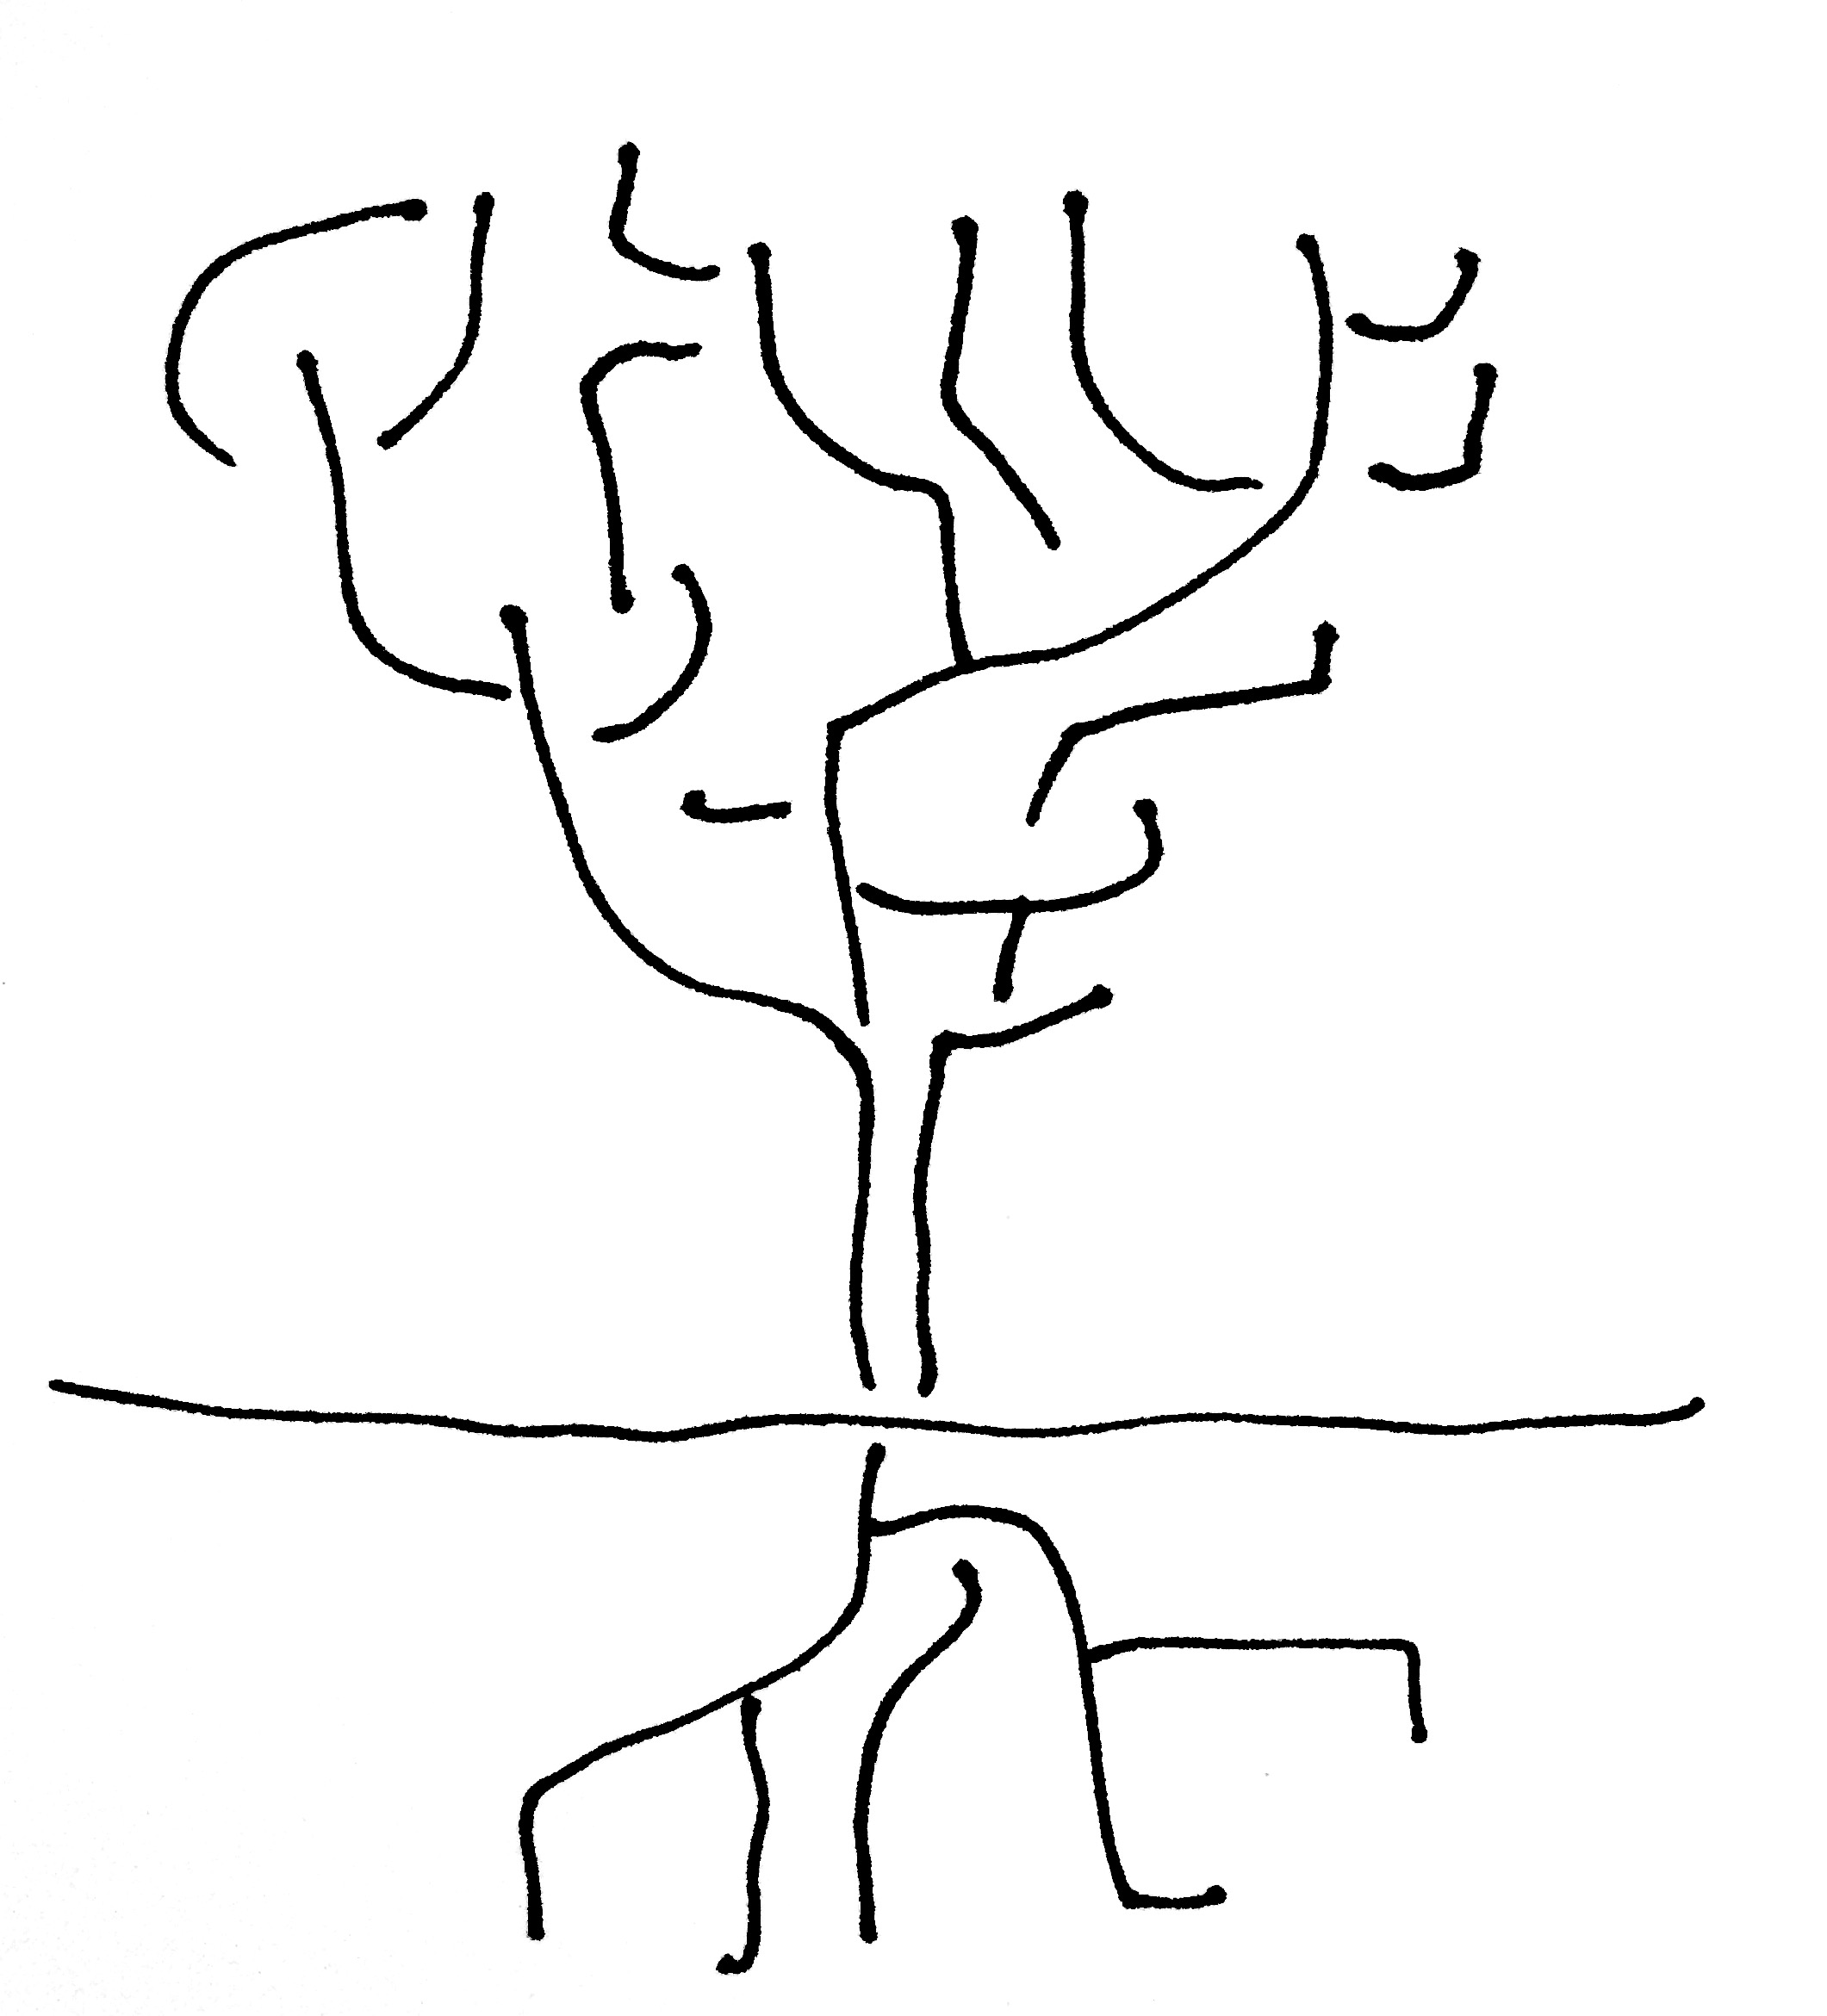
\includegraphics[width=1\textwidth]{/Users/federicocamarahalac/Documents/fd_work/text/waves/bin/img/dbtree.png}
\newpage

%------------------------------------------------------------------------------
%
%	BLANK PAGE
%
%------------------------------------------------------------------------------
\thispagestyle{empty}
\addtocontents{toc}{\protect\thispagestyle{empty}}
\clearpage
\newpage

%------------------------------------------------------------------------------
%
%	BEGIN EXTRAS
%
%------------------------------------------------------------------------------
\pagenumbering{roman}

%------------------------------------------------------------------------------
%
%	DEDICATION PAGE
%
%------------------------------------------------------------------------------

\chapter{Dedication}
For my mother and father, who have always taught me to never give up with my research, even during the most difficult times. Also to my advisor, Jaime Oliver La Rosa, without his help and continuous guidance, this would have never been possible. For Elizabeth Hoffman and Judy Klein, who always believed in me, and whose words and music I bring everywhere. Finally to Aye, whose love I cannot even begin to describe.
\newpage

%------------------------------------------------------------------------------
%
%	ACKNOWLEDGEMENTS PAGE
%
%------------------------------------------------------------------------------

\chapter{Acknowledgements}
I would like to thank my advisor, Jaime Oliver La Rosa, for his role in inspiring this project, as well as his commitment to research, clarity, and academic rigor. I am also indebted to committee members Martin Daughtry and Elizabeth Hoffman, for their ongoing guidance and support even at the very early stages of this project, and William Brent and Robert Rowe, whose insightful, thought-provoking input made this dissertation come to fruition. I am also everlastingly grateful to Judy Klein, for always being available to listen and share her listening. As well as to Aye, for her endless support and her helping me maintain hope in developing this project. I would also like to thank my parents, Ana and Hector, who inspired and nurtured my interest in music from a young age, and my sister Flor and my brother Joaquin who were always with me, next to every word. Finally, this dissertation could not have been possible without the support and help of my friends, some of which I would like to mention by name because they affected directly certain aspects of this text. I would like to thank Matias Delgadino and Lucia Simonelli, for their continuous layers of abstraction; Matias Borg Oviedo, for those endless conversations; Ioannis Angelakis, for his glass sculptures.

\newpage

%------------------------------------------------------------------------------
%
%	PREFACE PAGE
%
%------------------------------------------------------------------------------

\chapter{Preface}
\paragraph{Dataloquy (you don't need to \sout{write} this)}
(The initial title that explains how databases are everywhere) The name of the database. (Now think of the data, and the base, and how these relate) These words must point to two things placed one inside the other. (Is it base in data or is it data in base?) The base (of the data). A basement, a basis, a basic foundation for data. The house where data resides. (Is it the base or the data that is economical? Or both?) The addresses in which they are located. (Clearly, you are talking about pointers) The discretized space that guards data. (Guardians of space? This starts to look like a bad sci-fi thing\dots) Data as in the plurality of datum, and database as the plain (\textit{planicie} in spanish) or the lattice upon which the address space is laid for data. (Data under house arrest) Datum as in bit, as the zero or the one, and nothing in between (Are you sure there is nothing in the middle?) Data as in bytes, and the eight bits that follow it around (like ducklings without mom [\textit{pata} in spanish]) Data as in data types, the many names of the binary words representing the values of almost all numbers (and this `almost' is still more than enough (Some would disagree)). Data as in data structures and their unions, symbols, lists, tables, arrays, sequences, dictionaries, simultaneously pointing to their interfaces and their implementations and assemblage (The assembly is in order) Data as in files \textit{fichiers} in french, \textit{archivos} in spanish, and their kilobytes and megabytes (inside directories and folders, etc.) Data as in data flow and data streams (are there data fountains?) Data you translate from slot to slot, transmit from client to server to client, transduce to and fro with \obj{adc} and \obj{dac}, transcode from format to format (transgress from torrent to torrent) Data as in dataset for your algorithms to test, to improve, to fit, to make them more efficient, to teach them the right tendencies, to drive your models data-driven (You are driving me crazy) Data as in data banks (also its transactions and currency) Data as in data corpus (Oh, so it has body?) Data as in database (finally), basing gigabytes with models meant for system management and warehouses, repositories, terabytes, their mining, and their subsequent data clouds, clusters, spacing out into the (in)famous big data leap from bit to big.



% \begin{quote}
% \footnotesize
% \flushright
% \raggedleft
% \textit {
% 	I am sitting in a room different from the one you are in now. I am recording the sound of my speaking voice and I am going to play it back into the room again and again until the resonant frequencies of the room reinforce themselves so that any semblance of my speech, with perhaps the exception of rhythm, is destroyed. What you will hear, then, are the natural resonant frequencies of the room articulated by speech. I regard this activity not so much as a demonstration of a physical fact, but more as a way to smooth out any irregularities my speech might have.\footnote{Alvin Lucier. I Am Sitting In A Room. See: \url{https://en.wikipedia.org/wiki/I_Am_Sitting_in_a_Room}}
% }
% \end{quote}


\newpage

%------------------------------------------------------------------------------
%
%	END EXTRAS
%
%------------------------------------------------------------------------------

%------------------------------------------------------------------------------
%
%	BEGIN chapter*: Abstract
%
%------------------------------------------------------------------------------
\chapter*{Abstract}
\addcontentsline{toc}{chapter}{Abstract}
The aim of this dissertation is to understand the aesthetic agency of the database in music composition. I place my dissertation in relation to existing scholarship, artists, and developers working in the fields of music composition, computer science, affect, and ontology, with emphasis on the ubiquity of databases and on the need to reflect on their practice, particularly in relation to databasing and music composition. There is a database everywhere, anytime, always already affecting our lives; it is an agent in our aesthetic and political lives just as much as we are agents in its composition and performance. Database music lives in between computers and sound. My argument is that in order to conceptualize the agency of the database in music composition, we need to trace the history of the practice, in both its technical and its artistic use, so as to find nodes of action that have an effect on the resulting aesthetics. Therefore, this dissertation is composed of two main sections.

In the first section, I trace a history of database practices from three points of view. The first is from new media theory, emphasizing certain aspects of embodied theory which relate to the intersection between the database and the body. The second is from the history of the database in computer science, giving a panoramic view of the tools and concepts behind database systems, models, structures. The third is from their use in sound practices, describing different approaches to databasing from the fields of music information retrieval, sonification and computer music. In the second section, I discuss this agency under the broader concepts of sound, self, and community. These three axes are addressed in four sections, each with a different perspective. First I focus on listening, delineating Jean-Luc Nancy's ontology of sound in order to present the database as a resonant subject in a networked relation and community with the human. Second, I focus on memory, comparing human memory and writing with digital information storing, thus relating databasing and composition with memory, archives and their spectrality. Third, I analyze the performativity of databasing, understanding the database as gendered, in its temporality, repetition, and in its contingent appearance as style, skin, and timbre. In the last section, I revise the notion of music work, reflecting on the consequences of the anarchic and the inoperative in the community of database music.

% As an appendix, I develop an open-source library for multimedia composition that combines computer vision and timbre analysis algorithms to generate a database of descriptors, interpreting them as nodes in a network suitable for automated navigation.

%------------------------------------------------------------------------------
%
%	END chapter*: Abstract
%
%------------------------------------------------------------------------------

%------------------------------------------------------------------------------
%
%	TABLE OF CONTENTS
%
%------------------------------------------------------------------------------
\tableofcontents

%------------------------------------------------------------------------------
%
%	LIST OF FIGURES
%
%------------------------------------------------------------------------------
\cleardoublepage
\phantomsection
\addcontentsline{toc}{chapter}{List of Figures}
\cleardoublepage
\listoffigures

%------------------------------------------------------------------------------
%
%	LIST OF TABLES
%
%------------------------------------------------------------------------------
\cleardoublepage
\phantomsection
\addcontentsline{toc}{chapter}{List of Tables}
\cleardoublepage
\listoftables
\newpage

%------------------------------------------------------------------------------
%
%	END FRONTMATTER
%
%------------------------------------------------------------------------------
\mainmatter
\pagenumbering{arabic}

%------------------------------------------------------------------------------
%
%	BEGIN chapter*: Introduction ----
%
%------------------------------------------------------------------------------
\chapter*{Introduction}
\label{chapter:Introduction}
\addcontentsline{toc}{chapter}{Introduction}
This dissertation begins with a word (`database') and a proposition: Is there something we can call database music? This sudden jump from noun to adjective comes not without its audible retaliation, and I make no attempt to muffle it. The reader would perhaps forgive the clumsiness of my condition of composer in the midst of writing his dissertation, which made me jump to quickly at the opportunity to make some sound in this initial gesture. Nevertheless, there is a sound and we can listen to it.

In the literature that I have mined (for this dissertation is not only a text, but the sedimented layers of text that I initially traversed with keywords in database queries, such as ``\texttt{database AND music}''), the database has many histories and many names attached to it. I make no attempt to cover all of these, but I admit that I have (foolishly) tried: the subtitle does begin ``a history\dots.'' However, it is the `a' that would account for the gaps and missing parts to which this text is inevitably bound. It is also the `a' that accounts for the path that I begin delineating across the two nodes that compose the focus of this text: \textit{database and music}. Both nodes have their historical, technical, and aesthetical idiosyncrasies. The primary goal of this dissertation (if I dare to say that it has one) is thus to find where these intersect. The \texttt{AND} of the query had indeed much less results than the \texttt{OR}, which meant my quest was already promising some reduction. For instance, I indeed decided that the search would only pertain to situations in which computers were involved. Needless to say, not only was my search dramatically expanded through the plethora of database applications, the history of their systematization, and the ongoing struggle between models, it also opened up the programming world, and with it the history of programming languages, and of the computer itself. 

Upon this abysmal enterprise, I did as any musician would and started listening for the sound of databases. I realized that this is not just the sound of your computer reading its hard-drive: it is the sound made with its software. At this point, a network (and this is one of the key terms throughout this text) of sonic software had begun to appear. What this network pointed to, besides the key to open door number one, is a certain silence that much of the literature relating to databases in art continues to abide to: a sonic silence. This relates to the ``history, technology\dots'' part of the subtitle. In addressing this silence, I do not attempt to invalidate previous approaches \parencites{Man01:The}{Ves07:Dat}. On the contrary, these texts have shed light of the key concepts with which I have traversed the sonic software I present, the types of programming decisions I discuss, the various disciplines I place at the intersection of computers and music, and the plurality of shapes that have appeared in relation to databases: door number two. That is to say, through these authors, I introduce notions of embodiment, virtuality, and framing coming from posthumanism \parencite{Hay99:How} and new media theory \parencite{Han04:New}, in order to contextualize the role of the database within the practices of \gls{mir}, Sonification, and Computer Music. Each one of these disciplines has its own history and it is evidenced by the many conference proceedings and journals that I have (again) mined, as well as the various authors (most of them composers, and most of them programmers) that I refer to. In between these two, that is, in between my exploration of the database in new media theory, and its corresponding exploration within sound practices, I introduce the more technical evolution of the database, in order to develop a secondary concept that speaks of the performativity of databases: \textit{databasing}. I use this non-existing gerund to refer to all the actions that need to take place around databases, whether these are made by humans or not, referring mostly to these as \textit{databasers}.

After having reached this point, in which the intersection of the database and music was covered in terms of its facticity, as the evidence of a motion, the trace of the database, I could not help but noticing door number three. I began listening to a certain sound of networks, a certain resonance. This door refers to the next part of the subtitle ``\dots aesthetics of the database\dots'' and opened up to the complex world of sound, flipping this text upside down: \textit{music and database}. (Bang!) The meaninglessness of this reversal, at least semantically or even in terms of a database query, became precisely the point. The sound of databases that I delineate through the first two doors now reached a point where it faces a difference. I enter first with \poscite{Nan07:Lis} ontology of sound, with which I understand the networks of music software as resonant networks. With this move, the database sounds as a actor \parencite{Lat90:On} that reconfigures the way we think communities \parencite{Nan91:The}. The implications of this association led me to distinguish databases, memory, and archives, and find within their connections a spectral form of authority \parencites{Der78:Wri}{Der95:Arc}. The final move extends towards the activity of the (human) body, and the relationship between database, gender, and performance \parencite{But88:Per}. These three nodes (resonance, spectrality, and performance) encompass an aesthetics of the database that I situate around sound. 

Up to this point, my argument might seem to have arrived to an end: I contextualize and define database practices (chapter 1); I develop a technical overview of the performativity of the database into what I call databasing (chapter 2); I review the existing literature with emphasis on sound practices (chapter 3); I conceptualize sound in terms of resonance, networks, and community (chapter 4); I delineate the differences between database, memory, and archive, in order to present the spectrality of databases (chapter 5); I develop databasing in terms of performance, gender, and style in relation to databases (chapter 6). However, there is yet one more leap that the more adventurous reader might take with the final chapter of this dissertation. In chapter 7, I bring the discussion of database and music and database and music\dots to the latter part of the subtitle ``in music composition.'' With this chapter (a fourth door) I engage with the work of music composition. That is to say, with the history of the database in mind, I rethink the activity of composing \parencite{Vag01:Som}, the role of the composer \parencite{Lew99:Int}, and the operativity of the music work \parencite{Cas00:The}. The reader will be warned that this last chapter has no conclusions, let alone answers. Neither has it proper questions. It can be held as an attempt to incite, if anything, a provocation before the question.

I have already warned the reader of the clumsiness of a composer in the midst of writing, but that should not discourage neither academic rigor, nor literary thirst. I have thus included an exhaustive bibliography, two interludes, a transcription, and a postlude (work in progress), together with graphs, tables, and some snippets of pseudocode and sometimes working code. In the hope that you will continue reading these p\{age,ixel\}s, I will (simply) \xout{draft an} end \xcancel{to} these remarks.

%------------------------------------------------------------------------------
%
%	END chapter*: Introduction
%
%------------------------------------------------------------------------------

%------------------------------------------------------------------------------
%
%	BEGIN chapter: Database Art ----
%
%------------------------------------------------------------------------------
\chapter{Database Art}
\label{chapter:Database_Art}
% In order to define and contextualize database practices, I engage with the existing literature on data-driven art. Drawing mostly from media theory, I provide a sample of a variety of authors who have studied the use of databases in art. Specifically, I emphasize certain aspects of affect theory which relate to the intersection between the database and the body, in order to link database practice with sound and performance practices. 

% Therefore, in `databasing music,' I describe different approaches to music practices ---computer music, sonification, music information retrieval--- and their interrelation with software design, to show how some of the major breakthroughs of these practices are related to changes in data structures. In the last section of the chapter, I describe all layers of the concept of the database, from lower ---data structures--- to higher ---databases--- levels, and describe the basic algorithmic designs in between. Specifically, I argue that all of these layers constitute what I call the performativity of the database, which is what is incorporated in the practice of database music.
%------------------------------------------------------------------------------
%
%	END chapter: Database Art
%
%------------------------------------------------------------------------------

%------------------------------------------------------------------------------
%
%	BEGIN section: The Database In New Media Theory ----
%
%------------------------------------------------------------------------------
\section{The Database In New Media Theory}
\label{section:The_Database In New Media Theory}
% In this section I engage with the existing literature on data-driven art. In relation to new media, Manovich first considered the Database to be a new `symbolic form' of art \parencite{Man01:The}. The database became a term related to `internet' and `digital' art, and as such it was conceptualized in relation to interface design and interactivity. Hansen provided further insight to Database practices through theories of embodiment \parencite{Han04:New}. He claimed that since Manovich's theorizations did not take into account the Body as an active agent, human-computer interaction so far fell short of reaching its aesthetic potential. Vesna, Daniel and Lovejoy proposed a theorization of context within Database Art \parencite{Ves07:See,Dan07:The,Pau07:The,Kle07:Wai}. In their theorizations of interactivity in Database Art, they reassessed authorship in Digital Art. These authors later provided a panoramic view of database practices within the digital art world, and arrived at the broader term \textit{Database Aesthetics}. Since then, studies on database aesthetics have only been present in the existing literature in terms of data practices.
%------------------------------------------------------------------------------
%
%	END section: The Database In New Media Theory
%
%------------------------------------------------------------------------------

%------------------------------------------------------------------------------
%
%	BEGIN subsection: Database As Form ----
%
%------------------------------------------------------------------------------
\subsection{Database As Form}
\label{new_media}
\begin{quote}
	The world appears to us as an endless and unstructured collection of images, texts, and other data records, it is only appropriate that we will be moved to model it as a database ---but it is also appropriate that we would want to develop the poetics, aesthetics, and ethics of this database. \parencite[219]{Man01:The}
\end{quote}

To point to the origin of the database as it is known today is not an easy task. Certainly, databases are closely related to the history of computers, but they also relate to the history of lists. The common link between these two is the fact that they are written ---on a memory-card, on a page---, which would take its history to the origins of the written word\dots. However, there is a point where the history of storage takes an operational turn. At this point, the `word' becomes a type of data, and data begins to bloom exponentially, impulsing faster and more efficient storage and retrieval technologies. Database systems were modelled hand-in-hand with computer languages and architectures from the late 1950s until the present day, when they continue to be developed for almost all aspects of the business world.

In the artworld of the 1990s, the increasing availability of personal desktop computers ---with software suites, programming languages, and compilers--- resulted in the emergence of new media art. Lev Manovich \parencite{Man01:The} was the first media historian to argue that the database became the center of the creative process in the computer age. The database had become the content and the form of the artwork in \citetitle{Man01:The}. Furthermore, Manovich recognized that the artwork itself had become an interface to a database; an interface whose variability allowed the same content to appear in individualized narratives. Thus, he claimed that narrative and meaning in new media art had been reconfigured differently. Narrative became the trajectory through the database \parencite[227]{Man01:The}, and meaning became tethered to the internal arrangement of data.\footnote{Graham Weinbren writes that a database ``does not present data: it contains data. The data must always be in an arrangement\dots that gives the data its meaning'' \parencite[67-9]{Wei07:Oce}.} Therefore, for Manovich, the ``ontology of the world as seen by a computer'' \parencite[223]{Man01:The} was the symbiotic relationship between algorithms and data structures. As a consequence of the use of databases in art, the architecture of the computer was transferred to culture at large \parencite[235]{Man01:The}. Manovich's `database as symbolic form' thus became a technologically determined shadow that haunted much of new media.

%------------------------------------------------------------------------------
%
%	END subsection: Database As Form
%
%------------------------------------------------------------------------------

%------------------------------------------------------------------------------
%
%	BEGIN subsection: A Semiotic Trap ----
%
%------------------------------------------------------------------------------
\subsection{A Semiotic Trap}
\label{semiotics}
\img{one-to-many}{0.3}{
	Top: syntagm, paradigm, and their relation.
	Bottom: narrative, database, and their reversed relation.
}{Syntagm and Paradigm reversal}

In order to reveal the extent to which the presence of the database has a radical effect on narrative, however, Manovich reverses the semiotic theory of syntagm and paradigm that governed the first half of the 20th century \parencite[231]{Man01:The}. Quoting Roland Barthes' reading of Ferdinand de Saussure in \citetitle{Bar68:Ele}, Manovich describes the paradigm as a relation subjected to substitution ---because it depends on associations---, and the syntagm as a relation subjected to combination ---because it is an instantiation of concrete elements. For example, from the entire set of words in a language (the paradigm) the speaker constructs sentences (the syntagm): the paradigm is implicit (absent) and the syntagm is explicit (present). The relation between these two planes (of the paradigmatic and the syntagmatic) is established by the dependence of the latter on the former: ``the two planes are linked in such a way that the syntagm cannot `progress' except by calling successively on new units taken from the associative plane [i.e., the paradigm]'' \parencite[59]{Bar68:Ele}. Barthes gave several examples with different ``systems,'' one of which was the ``food system,'' which I will borrow in what follows. All the elements that compose a dish, for example, the ``set of foodstuffs which have affinities or differences within which one chooses a dish in view of a certain meaning'' comes to delimit the paradigm. However, the ``sequence of dishes chosen during a meal,'' or simply, what you are eating as you are eating it in a restaurant, comes to represent the syntagm \parencite[63]{Bar68:Ele}. However, when one looks at the restaurant's `menu', one can glance at both planes simultaneously: ``[the menu] actualizes both planes: the horizontal reading of the entrées, for instance, corresponds to the system [i.e., paradigm], the vertical reading of the menu corresponds to the syntagm'' \parencite[63]{Bar68:Ele}. A software menu, for instance, would come to represent both planes as well: the paradigm is the set of all possible actions the user might make within the specific context of the menu; the syntagm is the actual sequence of clicks that the user makes. 

Barthes' reading of Saussure is maintained in Manovich's description of the database. On the one hand, narrative is the syntagm since, at least in Manovich's rendition of narrative in the visual art world and the gaming world, it is the trajectory through the navigational space of a database. Furthermore, since this narrative is achieved by the interface, interface and narrative depend on each other: narrative thusly interlocks with the interface itself, and results on the conception of the interface-as-artwork. On the other hand, the database is the paradigm, since it represents the set of elements to be selected by the user. Materially, however, Manovich points to a reversal of these planes. Given the material presence of the database (i.e., the stored data), and given the hyperlinked quality of the user interface, the database becomes explicit (present) and narrative becomes implicit (absent, dematerialised).

For example, consider the case of the typical timeline-view of a video editor.\footnote{This example was used by Manovich in the late 1990s, and it is still valid today with most multimedia editing software.} Normally, the user creates a session and \textit{imports} files to working memory, creating a database of files ---video files, in this case. Once this database is in working memory, the user places on a timeline the videos, cutting, and processing them at will, until a result is desired, and an \textit{export} or a \textit{render} is made.\footnote{`Import,' `export,' and `render,' refer to processes that read from or write to the computer's disk.} The timeline where the user places the videos is a visualization of the set of links to the files; an editable graph that allows the user to locate in time the pointers to the elements on the database. This is what Manovich means by ``a set of links,'' because the user is not handling the files themselves ---as would be the case with an analog video editor, where the user cuts and pastes the magnetic tape---, but the extremely abstract concept of memory pointers. 

I consider this reversal to be valid, only on a certain quality of the relation itself, that is, as a shift from one-to-many to many-to-one \fsee{one-to-many}. The question of the materiality of the database and of the pointers depends on the materiality of data. Links or pointers have, for Manovich, a different (absent-like) status in relation to stored memory itself. This is because of a distinction between pointers and data on the basis of their use: pointers are of a different nature since they do not store data directly. Instead, they refer to the address in memory where a specific stored data begins. However, the mutual binary condition of pointers and data, and the fact that they are both stored in the same memory, reveal Manovich's reversal to be grounded on an equivocation. Pointers are, however functionally different, another data type. This fact comes from the Von Neumann architecture on which computers are constructed \see{programming}. If one understands them as moving bodies, it follows that pointers are `lighter' and travel much faster than other data types, which are `heavier' and slower to move. However, data types are not moving bodies at all, and thinking of them as such interlocks us in a semiotic trap: accepting this reversal means accepting the materiality of data.
%------------------------------------------------------------------------------
%
%	END subsection: A Semiotic Trap
%
%------------------------------------------------------------------------------

%------------------------------------------------------------------------------
%
%	BEGIN subsection: Digital Convergence ----
%
%------------------------------------------------------------------------------
\subsection{Digital Convergence}
\label{convergence}
\begin{quote}
	A mere `byproduct' of pleasure, entertainment is a hangover from the media epoch: a function that caters to our (\textit{soon to become obsolescent}) need for imaginary materialization through technology [which, in turn,] serves as a diversion to keep us ignorant of the operative level at which information, and hence reality, is programmed. \im \parencite[59]{Han02:Cin}
\end{quote}

I find in Manovich a silent allegiance to german media theorist Friedrich Kittler's concept of digital convergence. Digital convergence entails that the bodily resonance of media becomes obsolete in the face of absolute digital information storage. Thusly, it turns the human into a ``dependent variable'' \parencite[59]{Han02:Cin}. In the case of physical media, the human body was, for Kittler, directly shaped by media, and the limit of this `shaping' was set by the bodily limits of perception. The body became a by-product of media. However, in the age of digital convergence, of an ``absolute system of information'' \parencite[63]{Han02:Cin}, media remove this bodily limit of perception, making the human body a residual product. The body, then, becomes a residue of digital industries.

For example, the extents of this residual aspect of the human can be seen in writer Norman Klein's considerations of the author \parencite{Kle07:Wai}. Following Manovich's interface-as-artwork, Klein argues that since the reader gets immersed in data, she ``evolves pleasantly into the author'' \parencite[93]{Kle07:Wai}. Because the reader participates in the narrative, the result is a reconfigured concept of shared authorship. However, Klein continutes ``instead of an ending, the reader imagines herself about to start writing'' \parencite[93]{Kle07:Wai}. This surprising twist in Klein's consideration adds another layer of complexity, namely, the categorical difference between `writing' and `not-yet-writing.' In Klein's sense, narrative constitutes a promise of authority that equally blurs the roles of the writer and of the reader. Most importantly, this blurred authority is seen as a reflection of control and subordination of the human. In this view, the potentiality of authority arising from the trajectory through the database belongs neither to the reader nor to the writer: it is appropriated by the database. The roles of the reader and the writer fade into each other and vanish, allowing the database to be a dominant middle term. In other words, human agency is absorbed into a shadow, making the database the sole agent to which the human is subjected. In Klein's own words, the human is a slave to data, and as a consequence the human is economically colonized and psychologically invaded by the evolving force of computers, information, or technology in general \parencite[86-8]{Kle07:Wai}. Authority converges, too, in the age of digital convergence.

Media theorist Mark Poster defines technological determinism as the ``anxiety at the possibility of [the human mind's] diminution should these external [technological] objects rise up and threaten it'' \parencite[X]{Pos11:Int}. In other words, the fear or anxiety that the human is ultimately subjected to the power of technology. Understanding new media as digital convergence leads to reading the `new' in new media as the `digital.' In reaction to the anxieties that this convergence brings, and from an embodied approach where databases have an aesthetic agency in resonance with the human, in what follows I propose to shift the focus from narrative (interface) to performance (databasing), and to reconfigure the shadow of the database as a hybrid skin exposing the human and the non. 


%------------------------------------------------------------------------------
%
%	END subsection: Digital Convergence
%
%------------------------------------------------------------------------------

%------------------------------------------------------------------------------
%
%	BEGIN subsection: Bodiless Information ----
%
%------------------------------------------------------------------------------
\subsection{Bodiless Information}
\label{bodiless_information}
\begin{quote}
	The disembodiment of information was not inevitable, any more than it is inevitable we continue to accept the idea that we are essentially informational patterns. \parencite[22]{Hay99:How}
\end{quote}

Media theorist N. Katherine Hayles \parencite{Hay99:How} unearths the theoretical context of cybernetics, upon which the posthuman has been constructed throughout the 20th century. She identifies three waves of cybernetics, each governed by different concepts which helped build the undergirding structures of the technologically determined and disembodied literature in vogue in the 1990s. 

The foundational wave cybernetics (from 1945 to 1960) was built, among other concepts, on two main theories: Jon von Neumann's architecture of the digital computer \see{databasing} and Claude Shannon's theory of information. As ``a probability function with no dimensions, no materiality, and no necessary connection with meaning'' \parencite[18]{Hay99:How}, Shannon's formal definition of information within communication systems highlighted pattern over randomness \parencite[33]{Hay99:How}. Therefore, disembodied information became a signal to be encoded, decoded, and isolated from noise.

The word `cybernetics' [steersman] thus synthesized three central aspects: information, communication, and control. Since the human was seen as an information processing entity, it was ``essentially similar to intelligent machines'' \parencite[7]{Hay99:How}. Therefore, the conceptualization of the feedback loop as a flow of information came to put at ease notions of human subordination, thus arriving at the governing concept of first wave cybernetics: \textit{homeostasis}. In this sense, the ``ability of living organisms to maintain steady states when they are buffeted by fickle environments'' \parencite[8]{Hay99:How}, became a patch that simultaneously fixed computers as less-than-human, but also pointed to the anxiety of disembodied information that was growing underneath.

However, since the observer of the `feedback loop' became part of the flow of the system, in the second wave (from 1960 to 1980), cybernetitians reconfigured homeostasis into \textit{reflexivity}, that is, ``the movement whereby that which has been used to generate a system [becomes] part of the system it generates'' \parencite[8]{Hay99:How}. This became also known as autopoiesis (i.e., self-generation), based on writings by Humberto Maturana and Francisco Varela. This second wave leaves the feedback loop behind, since it considers that ``systems are informationally closed'' \parencite[10]{Hay99:How}. This means that elements in the system do not see beyond their limits, and the only relation to the `outside' environment is by the concept of a \textit{trigger}. In this sense, disembodied information was buried deeply into the organization of the system, and the system itself appeared in the form of a cyborg.

Shifting from triggers to artificial intelligence signaled the third wave of cybernetics (from 1980 onwards), whose central concept was \textit{virtuality}. Development of cellular automata, genetic algorithms, and principally, emergence, led to the formation of the posthuman, or an embodied virtuality. However, in Hayles view, the underlying premise of this `posthuman' is that the human can be articulated by means of intelligent machines \parencite[17-8]{Hay99:How}. In turn, reconfiguring the concepts of body, consciousness, and technology as inherent to (post-) human life, Hayles argues for the impossibility of artificial intelligence to serve as a proxy for the human. Hayles objective is, then, to dismantle cybernetics from its (relative) assumptions, questioning its major achievements over the years and thereby opening the field for new considerations of the body and its material environment within cybernetics, and by extension, of the body in new media:

\begin{quote}
	My dream is a version of the posthuman that embraces the possibilities of information technologies without being seduced by fantasies of unlimited power and disembodied immortality, that recognizes and celebrates finitude as a condition of human being, and that understands human life is embedded in a material world of great complexity, one on which we depend for our continued survival. \parencite[5]{Hay99:How}
\end{quote}

While her work is focused on the literary narratives that were built in parallel with cybernetics, she leaves incursions in new media theory for other media theorists. This is where Mark B. N. Hansen comes in.

%------------------------------------------------------------------------------
%
%	END subsection: Bodiless Information
%
%------------------------------------------------------------------------------

%------------------------------------------------------------------------------
%
%	BEGIN subsection: Embodying Databasing ----
%
%------------------------------------------------------------------------------
\subsection{Embodying Databasing}
\label{embodiment}
As I describe above, Manovich arrives at this notion of the interface-as-artwork by opposing database and narrative on the semiotic grounds of the reversal of the paradigm and syntagm. In turn, media theorist Mark B. N. Hansen \parencite{Han04:New} notes that the interface-as-artwork constitutes a disembodied ``image-interface'' to information in which the process of information itself (in-formation, giving form) is overlooked. Hansen locates the source of this disembodied conception in Manovich's implicit ---but nonetheless evident--- premise of the overarching dominance of cinema in contemporary culture, which results in a ``disturbing linearity [with] hints of technical determinism'' \parencite[36]{Han04:New}.

For example, Manovich argues that standardization processes originating from the Industrial Revolution have shaped how cinema is produced and received. Attuned to the perceptual limits of the body, the standardization of resolution can be seen (image dimensions, frames per second, and aspect ratio) and heard (audio bit depth, sampling rate, and number of channels). In this sense, the moviegoer and by extension, the listener became industrial by-products, determined by the massively produced electronic devices used for recording and playing. As I have described with Kittler's technological determinism, the devices driven by industrial forces, therefore shaped the body, and as an extension, the aesthetics of cinema. 

For Manovich, due to the internal role of the database, the logic of new media is no longer that of the factory but that of the interface. Through the interface to a database, the user is given access to multiplicities of narrative, and thusly, to endless information. The user is granted the power of the database, making in Manovich's eyes the database an icon of postmodern art. In other words, on an aesthetic level, while mass-standardization and reproducibility of media ---the ``logic of the factory'' \parencite[30]{Man01:The}--- shaped the form of cinema, post-industrial society and its logic of individual customization, shaped the database form. At the bodily level, cinema standardized perception of the passive body, and database individualizes experience. However, this individualized experience still constitutes a technological `shaping' of the body, a shaping that is exploded into every user quietly sitting behind the screen.

In opposition to this passivity of the body, Hansen describes images as something that emerges out of the complex relationship between the body and some sort of sensory stimulus. In radical disagreement with Manovich, Hansen considers that the image has become a process which gives form to information, and that this process needs to be understood in terms of the body as a filtering and creative agent in its construction. Drawing from Henri Bergson's theory of perception, and in resonance with cognitive science, Hansen defines the function of the body as a filtering apparatus. Under this conception, the body acts on and creates images by subtracting ``from the universe of images'' \parencite[3]{Han04:New}. Image creation is world creation, and it is not necessarily in contact with the reality that surrounds the body (or the reality of the body), but it is a result of the embodiment of a virtuality that is inherent to our senses. In other words, through this filtering activity, the body is empowered with ``strongly creative capacities'' \parencite[4]{Han04:New}. The world is a virtuality that is constructed with our senses and our body. The world can only appear if it appears to the body. Therefore, instead of being a passive node, the body actively \textit{in-forms} data as information (Hansen's word play). The databaser (database user) makes information out of data by precisely embodying the performative act that I call databasing. 


%------------------------------------------------------------------------------
%
%	END subsection: Embodying Databasing
%
%------------------------------------------------------------------------------

%------------------------------------------------------------------------------
%
%	BEGIN subsection: Filtering And Framing ----
%
%------------------------------------------------------------------------------
\subsection{Filtering And Framing}
\label{framing}
\begin{quote}
	The activity in the receiver's internal structure generates symbolic structures that serve to frame stimuli and thus to \textit{in-form} information: this activity converts regularities in the flux of stimuli into \textit{patterns} of information. \parencite[76]{Han02:Cin}
\end{quote}

The activity of framing, according to Hansen, must be differentiated from that of observation. In this way, ``information remains meaningless in the absence of a (human) framer,'' \parencite[77]{Han02:Cin} and framing becomes a resonance of the (bodily) singularity of the receiver. Quoting MacKay's \textit{Information, Mechanism, Meaning} (1969), the meaning of a message

\begin{quote}
	\dots can be fully represented only in terms of the full basic-symbol complex defined by all the elementary responses evoked. These may include visceral responses and hormonal secretions and what have you\dots an organism probably includes in its elementary conceptual alphabet (its catalogue of basic symbols) all the elementary internal acts of response to the environment which have acquired a sufficiently high probabilistic status, and not merely those for which verbal projections have been found. \parencite[78]{Han02:Cin}
\end{quote}

It is with this conception of framing that Hansen describes precisely that information always requires a frame:

\begin{quote}
	\dots this framing function is ultimately correlated with the meaning-constituting and actualizing capacity of (human) embodiment\dots the digital image, precisely because it explodes the (cinematic) frame, can be said to expose the dependence of this frame (and all other media-supported or technically embodied frames) on the framing activity of the human organism. \parencite[89-90]{Han02:Cin}
\end{quote}

Therefore, in the context of Kittler's digital convergence, framing prevents the human from being rendered a dependent variable. To the contrary, the framing function of the human body is the possibility condition for the digital to become information. The frame, as Hansen describes, is the human body filtering images from the world, and creating a virtual image that gives form to data. The frame needs to happen as a relation, and thus, it is the temporal instantiation of a process.

%------------------------------------------------------------------------------
%
%	END subsection: Filtering And Framing
%
%------------------------------------------------------------------------------

%------------------------------------------------------------------------------
%
%	BEGIN subsection: An Embodied Database ----
%
%------------------------------------------------------------------------------
\subsection{An Embodied Database}
\label{funeslude}

% EH:
% 
% Why does Irineo's isolation preclude a replaying of any infinitesimal
% moment? Your story is poetic and powerfully metaphoric such that I get
% your point without fully understanding how the story demonstrates it
% alas. Thanks!

\begin{quote}
	I suspect, nevertheless, that he was not very capable of thought. To think is to forget differences\dots \parencite[2]{Bor42:Fun}
\end{quote} % 4/7/2018 10:31:06

The importance of memory ---and forgetfulness--- can be represented by Jorge Luis Borges's famous 1942 short story, \textit{Funes, the memorious} \parencite{Bor42:Fun}. Due to an unfortunate accident, the young Irineo Funes was ---``blessed or cursed'' as Hayles points out \parencite[156]{Hay93:The}--- with an ability to ``remember every sensation and thought in all its particularity and uniqueness '' \parencite{Hay93:The}. A blessing, since a capacity to remember with great detail is certainly a virtue and a useful resource for life in general; a curse, because he was unable to forget and, as a consequence, he was unable to think, to dream, to imagine. Throughout the years, he became condemned to absolute memory, and so to its consequence, insomnia:\footnote{In the prologue to \textit{Ficciones}, Borges writes that this story is a long metaphor of insomnia: ``Una larga metáfora del insomnio'' \parencite{Ovi19:Mem}.} he was secluded in a dark and enclosed space so as not to perceive the world. Hayles focuses on one aspect of the story, namely, the fact that Funes invented ---and begun performing--- the infinite task of naming all integers, that is, of giving a unique name ---and sometimes, last name--- to each number without any sequential reference. According to how Hayles describes it, by carrying out his number scheme, Funes epitomizes the impossibilities that disembodiment brings forth. As Hayles writes, ``if embodiment could be articulated separately from the body \dots it would be like Funes's numbers, \textit{a froth of discrete utterances registering the continuous and infinite play of difference}'' \im \parencite[156-159]{Hay93:The}. The point that Hayles touches upon can be seen as the limits and fragility of embodied memory, as well as the need to forget, in opposition to an embodiment `outside' the body (disembodiment), that would require no need to forget. We will see how the difference between forgetting and erasing relates to the database. In that Manovichian world which ``appears to us as an endless and unstructured collection of images, texts, and other data records'' \parencite[219]{Man01:The}, this idea would be perfectly viable. Indeed, data banks have already been growing exponentially much in the same way as Funes' memory. This capability of accumulation without the need for erasure is enabled by the database structure inherent in computers. However, the distinction that Hayles presents is crucial: data is not information because information needs to be embodied, and with that embodiment comes the need to forget. In sum, on one hand, a disembodied data bank can have all the uniqueness and difference that is available by the sum of all cloud computing and storage to date; however, on the other hand, embodied memory is available by the human capacity to forget.

Matías Borg Oviedo \parencite{Ovi19:Mem} relates this incapacity for thought to the negation of narrativity itself, thus finding in the image of Funes a hyperbole for contemporary subjectivity \parencite[5]{Ovi19:Mem}, where there is no room for narration, only data accumulation. In this sense, narrativity can be seen as that which resides in the threshold between knowledge and storage. I believe this distinction stems precisely from the difference between information and data. The process of information, of giving form, requires a certain temporality that is not that of the perceptually immediate and extremely operative zero-time of the \gls{cpu}. Within the zero-time of computer operations (within a millisecond) there simply is no \textit{time} for narration, only for addition or increment. Narrative is temporal ---happening as a historical process--- and algorithms are atemporal ---operating in an constant now. Since neither data structures nor algorithms operate outside the confines of the millisecond, they can't spare time to think and, likewise, they can't forget to count. Counting is all they do, so they cannot tell stories: the difference in the same spanish word \textit{contar números} [to count numbers] and \textit{contar historias} [to tell stories]; or, ``if a German pun may be allowed: \textit{zählen} (counting) instead of \textit{erzählen} (narrating)'' \textcite[128]{Ern13:Dig}. Therefore, Funes' accumulative memory represents the overflow of the now, the totally blinding transparency of the world, and an absolute memory that precludes narration. Because he accumulates data of the world in its totality, he does not have time to think: ``to think is to forget differences'' reads the quote above. The only one in Borges' story who actually thinks is the narrator, to which we can add: Funes could not have told this story himself in first person narrative.\footnote{It is worth noting how Oviedo finds in Funes a premonitory `antithesis of the writer' himself: the latter (blind) Borges could find himself immersed in a constant flow of narrativiy \parencite{Ovi19:Mem}.} Thus, we can ask ourselves if this hyperbolic `light' of the Funesian `absolute memory' is not a premonitory figure of the database.\footnote{In this sense, Funes is a bit like an Oracle ---pun intended with the other \gls{oracle}---, with absolute knowledge of the past and the future, but with no time to think\dots} Because of this antithetical condition between databases and narrative, Manovich proposed that the database became a form on its own, in opposition to narration. To the extent that `database form' as a category that identifies art using databases, this can be considered accurate. However, considering this distinction between embodied and disembodied memory that resides in the ability to narrate, databases are inherently deprived of narration. Making art with databases is making them dance (see below). Therefore, to what extent is `database music' in itself a contradiction if we consider `music' to be a form of writing? I will leave this discussion for a later chapter \see{chapter:section-4}.

This Funesian database can also be understood in relation to what Gayatri Chakravorty Spivak \parencite{Der76:Of} writes about forgetfulness. She notes in Nietzsche the `joyful' and `affirmative' activity that constitutes forgetfulness as being twofold. On the one hand, this activity is a ``limitation that protects the human being from the blinding light of an absolute historical memory,'' and on the other, it is ``to avoid falling into the trap of `historical knowledge''' \parencite[xxxi]{Der76:Of}. The `historical' here is an ``unquestioned villain,'' which takes two forms: one ``academic and preservative,'' the other ``philosophical and destructive'' \parencite[xxxi]{Der76:Of}. For Nietzsche, as Spivak notes, forgetfulness is a choice that comes as a solution: an ``antidote'' to the ``historical fever,'' or the ``unhistorical,'' that is, ``the power, the art of forgetting\dots'' \parencite[xxxi]{Der76:Of}. I propose an imaginary experiment that would add some noise to Borges' short story, however utterly fantastic his writing was. One thing that can be read from the story is that, in order to seclude himself from perceiving the world, or better, in order to forget the world altogether, Irineo stayed in the darkness of his room. This is how he cancelled light, a quite powerful stimulus if memory-space is to be optimized for the purpose of, say, getting some sleep. However, there is little to no mention of the sonic environment in which Funes was embedded ---somewhere in the outskirts of the quiet Uruguayan city of Fray Bentos. In fact, the only sonic references are focused on the narrator's perspective, referring to Funes' high-pitched and ---due to his being in the darkness--- acousmatic voice. To a certain extent, we might think of Funes' high-pitched (at least this is how the narrator heard it) voice as a hint to the highlighted overtones that links Borges' ``long metaphor of insomnia'' with ``the `laughter' of [Nietzsche's] Over-man [that] will not be a `memorial or\dots guard of the\dots form of the house and the truth\dots He will dance, outside of the house, this\dots active forgetfulness'' \parencite[xxxii]{Der76:Of}. Nonetheless, Funes is deprived of this forgetfulness, and thus cannot go outside, let alone laugh or dance.\footnote{The acousmatic quality of Funes' voice will not be touched here, but it is indeed a good point of departure for another time.} By locking himself inside a room he would have managed to attenuate sound waves coming in from outside. Notwithstanding his isolation ---a house arrest---, sound waves are actually very difficult to cancel.

\sout{(} It is interesting to compare Funes' attempt to filter out the world with John Cage's quest for silence. An interesting experiment would have been to have John Cage take Irineo to an anechoic chamber and ask him what he can remember then. From Cage's own experience, we can guess that Funes would effectively remember his own sounding body. Kim \textcite{Cas00:The} writes that ``[Cage's] experience in an anechoic chamber at Harvard University prior to composing 4'33'' shattered the belief that silence was obtainable and revealed that the state of `nothing' was a condition filled with everything we filtered out'' \parencite[14]{Cas00:The}. It is interesting to place an 80 year-old Irineo in David Tudor's premiere at Maverick Concert Hall in Woodstock, NY, infinitely listening to 4'33'' \sout{)}

It is very unlikely ---but nonetheless possible--- that Borges was aware of American acoustician Leo Beranek's research for the US Army during World War II, that is, when the first anechoic chamber was built.\footnote{\url{https://en.wikipedia.org/wiki/Leo_Beranek}} Furthermore, even if he managed to isolate himself completely from the world by cancelling perception altogether, Funes would have been with his memories (he was not deprived of \textit{anamnesis}, the ability to remember), which were not discrete, but continuous iterations of the world he had accumulated over the years. What this means is that all the sounds he had listened to would be available to his imagination. As far as we can learn from the narrator, while \textit{smell} is referenced to in the story, \textit{sound} was nonetheless out of Funes' concerns. Therefore, one thing we can ask ourselves is how the world would sound for Irineo Funes? The task is not difficult to imagine: the world would be inscribed in poor Irineo's memory in such an infinitely continuous way that each fraction of wave oscillation would be different, unique, leaving no space for repetition of any kind. For example, one of Irineo's concerns was to reduce the amount of memories on a single day, which he downsized to about seventy thousand\dots. What would be Funes' sample rate? What frequencies could he be able to synthesize? All sounds (and all that can be registered) would be listened to completely, with every infinitesimal oscillation of a wave pointing to the most utterly complete scope of imaginable references. A complete state of listening. In fact, we might not be able to call it listening any more. Not even signal processing. An infinitesimal incorporation of sound is unthinkable. Within such total listening there would be no possibility for thought, no processing of any kind, and no synthesis: only infinite accumulation and storage. On the one hand, no matter how accurate our embodied listening might be, we are bound to miss some motion, some waves would pass through us and we would be busy forgetting to register them. On the other hand, if such a recording were humanly possible, thinking would cease to be so. This can be thought of as the intersection of the finite with the infinite: while Funes' nonhuman memory corresponds to a dynamics of the infinite, his human body is quite human. Funes is not deprived of this finitude, and existed (fantastically) on a ghostly liminality. This liminality grows more and more evidently throughout the story, hand in hand with the cumulative growth of the Funesian database, all the way until the end, in a sort of Moore's Law of data congestion, saturating completely in an utterly human pulmonary congestion \parencite{Ovi19:Mem}.



% Studies in cognitive psychology \parencite{Wes08:How} consider forgetting to be an adaptive and functional activity. Nonetheless, it is considered as a ``failure'' of certain search processes on account of an inability to recall information from memory. This failure is a mystery when it comes to human memory ``it is unclear what really happens to old, disused or deliberately ignored memory traces ---they might be retrievable, they might be lost, but no-one can tell'' \parencite[292]{Wes08:How}. Nevertheless, the mystery vanishes the moment memory becomes externalized in writing or in archives, because it becomes extinguishable.




%------------------------------------------------------------------------------
%
%	END subsection: An Embodied Database
%
%------------------------------------------------------------------------------

%------------------------------------------------------------------------------
%
%	BEGIN subsection: Closing Remarks ----
%
%------------------------------------------------------------------------------
\subsection{Closing Remarks}
\label{generated}
Despite Manovich's technologically determined considerations of the database as form, he notes a fundamental aspect of the use of the database when he expresses that data need to be collected, generated, organized, created, etc: ``Texts need to be written, photographs need to be taken, video and audio need to be recorded. Or they need to be digitized [and then] cleaned up, organized, and indexed'' \parencite[224]{Man01:The}. In this sense, he begins to describe the actions that need to be performed around data, what I call databasing \see{databasing}, which connotes the use of databases in terms of their performativity \see{chapter:section-6}. He even goes further and proposes that this activity has become a ``new cultural algorithm,'' \parencite[225]{Man01:The} \fsee{manworld}.
% Following this line of thought, artist Victoria Vesna \parencite{Ves07:See} argues that creating a memory bank is a means of testifying to our existence \parencite[25]{Ves07:See}. 

\img{manworld}{0.6}{
	The world is mediatized, stored in some media (film, tape), then digitized into data, then structured into a database. The result is the world represented by the database.
}{Manovich's cultural algorithm}

While Manovich calls for an ``info-aesthetics'' \parencite[217]{Man01:The}, as well as a poetics, and ethics of the database, neither Manovich nor the following generation of media artists and theorists could carry out an exhaustive account of an aesthetics of the database. Several authors continue to abide by Manovich's claim that the aesthetics of the database, or the database as form, is a symptom of the uncritical use of database logic throughout the visual art world of the 1990s. It is in hindsight that his argument can be understood as grounded on the same disembodied constructions that prevent him from including human agency in his account. In any case, his contribution to the literature on the role of databases in new media have led us to this point of inflexion, in which we can consider different points of view regarding the topic of databases. My revision of this algorithm will come later in this dissertation \fsee{unwork}. In what follows, I will explore the more technical aspects of databasing, in order to trace a connection between the literature on sound-based computer practices with that of the development of databases over the years. In this way, I bring the discussion of databases into the sonic sphere.

%------------------------------------------------------------------------------
%
%	END subsection: Closing Remarks
%
%------------------------------------------------------------------------------

%------------------------------------------------------------------------------
%
%	BEGIN section: Databasing And The History Of Databases ----
%
%------------------------------------------------------------------------------
\section{Databasing And The History Of Databases}
\label{section:Databasing_And The History Of Databases}
% This is why I now focus on Database practices before entering the `age of information' (McLuhan 1964, Chion 1994, Manovich 2001, Simons 2002, Vesna 2007, Paul 2008, van Dijck 2017). I define two precursors of the database as `statistics' and `archival practices.' First, I contextualize briefly the practice of statistics, and describe the notions of `sampling' and `data collection,' in order to provide a glance on what I consider the origin of data-based practices. Then, I begin relating the concept of the Archive ---as presented by Derrida (Archive Fever, 1995)---, so as to deepen the understanding of the principles involved in archival practices. I describe the main technical concepts behind Database Navigation and provide use cases from both appendices A and B, the former relating to joint image and audio databases, and the latter to text databases. I then reflect on the quality of this navigation in relation to the type of navigation and results that they obtain.

%------------------------------------------------------------------------------
%
%	END section: Databasing And The History Of Databases
%
%------------------------------------------------------------------------------

%------------------------------------------------------------------------------
%
%	BEGIN subsection: Databasing: The Performance Of The Database ----
%
%------------------------------------------------------------------------------
\subsection{Databasing: The Performance Of The Database}
\label{databasing}
\begin{quote}
	The first step in working with a database is the collection and assembly of the data\dots. Sorting determines the sequence of presentation, while filtering gives rules for admission into the set presented [,] resulting in a database that is a subset of the ``shot material'' database. Editing is selecting from the database and sequencing the selections\dots. To go further: for a filmmaker the term ``cutting,'' as ``editing,'' loses its meaning, and ``sorting,'' ``assembling,'' and ``mapping'' become more apt metaphors for the activity of composition. \parencite[71]{Wei07:Oce}
\end{quote}

Like Manovich, Weinbren finds a redefinition in filmmaking impulsed by the selection processes that the database calls for: data collection, generation, and assembly. Weinbren further breaks the selection process into sorting and filtering. With this new terminology, Weinbren makes a linguistic shift from `editing' and `cutting,' to `sorting,' `assembling' and `mapping.' This linguistic shift is significant in the sense that it highlights the practice that is `under' the filmmaker: databasing. 

Databasing is a term I have chosen that best describes the practice of the database, that is, a term that includes the elements and actions of database practices, together with their temporality. The elements of databasing are the different data types and structures that build more complex database systems. The actions of databasing are, on the one hand, the type of operations that a database allows, and on the other, the bodily activity that occur before and after these operations. That is to say, since the operational level occurs below the perceptual threshold of the body, I consider the actions surrounding the immediacy of computations to be defining aspects of databasing.

\subsubsection{Data types and structures}

Depending on the programming language, data types may or may not be part of a data structure, and they store different types of values such as \texttt{int, float, char}. These types are then interpreted in binary language by the compiler. Grouping these types into larger sets results in \texttt{array}s. For example, in the C programming language, programmers `declare' variables first ---e.g., \texttt{unsigned char age}--- and then `initialize' them with some data ---e.g., \texttt{age=30}. A simple variable like one's `age' needs only one value, and given that the \texttt{unsigned char} data type only stores values from 0-255, it is safe to use in this case: no age can be negative, no human can live longer than 255 years.

A data structure is a set of data types kept generally in contiguous slots in memory space. It is built for fast allocation and retrieval. A very simple data structure can be thought of as, for example, a person's name together with an age \lsee{person}.

\begin{flushleft}
\small
\begin{lstlisting}[caption={An example of a data structure in the programming language C. It is named \texttt{Person}, and it holds two variables: \texttt{age} and \texttt{name}, respectively a positive integer and a string of up to 128 characters.},captionpos=b,label={lst:person}]
typedef struct Person {
	unsigned char age;
	char name[128];
} Person;
\end{lstlisting}
\end{flushleft}

\subsubsection{Temporality of Databasing}

At this point it is important to refer to the higher or lower levels of computer software. A software that is `higher' means that its simplest operations are composed of multiple smaller operations. The user can thus `forget' about certain complexities that come from low-level programs, such as memory management. In this sense, low-level programs operate `closer' to hardware, and programmers need to work at a more granular level. While the above data structure contains low-level features such as setting the size of the name array, it releases the programmer from thinking binary conversion. This means that unless you are changing values directly on the memory card (which is unthinkable), there will most likely be an underpinning software layer. 

The speed of regular house computers is so fast that high-level operations happen below the perceptual level (generally below 1-2 milliseconds), hence, for example, the capability for real-time audio processing at high quality sample rates. Therefore, the temporality of activity before and after potentially very large computations feels almost immediate. This means that the body continues almost as if nothing had happened besides a click, or besides the pressing of a key. The immediacy of computation is a feature, certainly, for arriving at extremely fast operations in no time (or zero-time). It is what feels like `magic' around computers: ask a computer to count to a 1000, and it already has\dots. 

However, it may become a bug if we consider the computer as a tool to understand the world. As Manovich claimed, the world understood with computers is not only one that is presented in binary terms, it is one constructed upon a specific set of data structures with their set of algorithmic rules. The better and more efficient the data structure is, the better and faster the algorithm. In this light, it can be argued that software development is essentially data structure development. At every software release, the software becomes more efficient, using less or more restricted memory space, etc., affecting the scope of its functionality as well as the speed at which it runs. Glancing at the evolution of software in terms of data structure efficiency, therefore, is glancing at a constantly accelerating stream of bits. Because it is immediate, software is incorporated immediately, thus narrowing the temporal window for framing.

This is why the temporality of databasing is context-dependent. As Hansen pointed out, the world can only appear if it appears to the body \see{embodiment}. Data structures, therefore, are very efficient storage devices that have no relation to worlds in themselves, but that are the condition for the possibility of world creating with computers. In this way, the programmer feeds into the computer a notion of world that is then returned by the computer's performance. In each data structure there is a result of a feedback network. One one hand, this network refers to the history of software development, in the sense that each software release is a instance of the much larger event that is software in general. On the other, the network links this history with the practice at hand for which the software is being designed. The sound of a computer music oscillator, for example, even if it were programmed today from scratch, would have embedded histories of computer software design, computer music history, etc.

What is important to note here, is that these interrelations of what is \textit{already there} in software development can be thought of as resonances colliding their way into stability; a stability that emerges not only as a `stable release' of the code, but also as the condensed multiplicity of worlds that is displaced into a software package. Therefore, data structures are world-making and world-revealing devices that engage with our own capacity for virtuality, and thus they are nodes in our world-making networks.


\subsubsection{Databasing and Writing}

As with other new media, the terminology used to describe computer memory is often borrowed from earlier media practices like printed text: reading, writing, and erasing. Computer memory thus shares with writing the property of hypomnesis, that is, of displacing the role of human memory with an external non-human device. In the case of the computer memory however, the scale of this displacement is extremely large, both in terms of the amounts of data that can be stored and the speed with which it can be stored. For example, the 40-bit long 4000 numbers that Von Neumann was aiming at for their memory `organ' ---which was more than plenty for the computational purposes required at the time--- represents around 16 Kilobytes, something which today might seem absurd in comparison to current computer storage capabilities that can be found in the case of cloud computing. In light of this fact, we might ask ourselves how is human work transformed through interaction with these massive external memories? Database practice has direct effects on temporality and on memory. Therefore, when designing computer software for art, the way in which data is structured, together with the speed and design of data flow, has significant effects on the temporality of art altogether as a practice. 

I have proposed that memory and its storing of instructions and information what enables the computer as such. The simplicity of this synthesis of data and command in Von Neumann's architecture, led to its implementation in not only the computer for which he had intended, also the regular computer as we know it today. Without this architecture, computers would only be able to perform very simple arithmetic operations (like pocket calculators). That is to say, without the computer's ability to store data (the memory organ), the partial differential equations that Von Neumann was aiming at solving would not have been possible. In these equations, the next value of the solution depends on the present value. Therefore, when iterating through every step of the solution, the function in charge of solving the equation needs to access the present value, change it, output the next value, and finally update the present value with the outputted result \see{lst:neumann}. Therefore, in order to provide such solutions, Neumann proposed that: ``not only must the memory have sufficient room to store these intermediary data but there must be provision whereby these data can later be removed'' \parencite[3]{von46:Pre}.

\begin{flushleft}
\small
\begin{lstlisting}[caption={Pseudocode showing a routine whose next value depends on the present value.},captionpos=b,label={lst:neumann}]
present = 0
next = 0
iteration {
	output = next = function() = present
	present = next
}
\end{lstlisting}
\end{flushleft}


\subsubsection{The Von Neumann Architecture}

\begin{quote}
	Inasmuch as the completed device will be a general-purpose computing machine it should contain certain main organs relating to arithmetic, memory-storage, control and connection with the human operator. It is intended that the machine be fully automatic in character, i.e. independent of the human operator after the computation starts \parencite[1]{von46:Pre}.
\end{quote}

Data structures are the turning point of the history of the database. Their appearance enabled the performance of automated algorithms. Within the history of computer technology, data structures begin to appear since Jon Von Neumann's designs of the computer architecture \parencite{von46:Pre}. Von Neumann and his team implemented Alan Turing's original concept for a general-purpose computing machine. Of the ``certain main organs,'' it is memory-storage what enables the computer's architecture as we know it today. On one hand, the storage unit of the computer allows data to be written and erased in different locations and times. On the other, the stored data can be not only values to be used during computation, but also includes the algorithmia itself, that is, the commands ---functions, operations, routines, etc.--- which are used to access and process data for computation. Thus, the interaction of data and command is what defines data flow inside the computer.

Consider, for example, how curator Christiane Paul describes the database as a ``computerized record-keeping system'', that is, ``essentially a structured collection of data that stands in the tradition of ``data containers'' such as a book, a library, an archive'' \parencite[95]{Pau07:The}. However, when Paul suggests that databases are simply an instance of data collection this only points to the passivity of the container, and not to the potential that it has. An good analogy would thus be a book with the capacity to read itself, if reading were going through every letter in an orderly fashion. A database can also be understood as a library with no need for librarians because all queries are immediate; or, an archive without archeion. These considerations will be developed in the next chapter. While the more general practices of collecting and classifying data are part of the practice of databasing, on some level of the computer architecture, databasing comprises data flow within the Von Neumann architecture. This fact marks a distinction that is better seen in relation to networks. Extending computers via networks like the Internet makes databasing a global activity that expands and changes with every user. This is why I propose that databasing reconfigures the passivity of data containers such as books, libraries, and archives, with a powerful agency that resonates aesthetically.

In order to understand how databases have changed the way we think of earlier types of containers, we need to revise the differences between database models in time. By doing this, I plan to reconfigure the notion of database system. In general, database systems have been used in businesses, namely for administration and transaction. However, narrowing database systems this way raises the similarities or differences between systems to the level of the interface. I propose to delve into the structures of the models to find how the computer itself can be thought of as a database tree, and databasing can be thought of as the activity around databases, or simply: \textit{database performance}. The main purpose of the following account is to understand how computer-based sound practices have participated as a particularly resonant branch of the database tree.


%------------------------------------------------------------------------------
%
%	END subsection: Databasing: The Performance Of The Database
%
%------------------------------------------------------------------------------

%------------------------------------------------------------------------------
%
%	BEGIN subsection: A Database Tree ----
%
%------------------------------------------------------------------------------
\subsection{A Database Tree}
\label{programming}
The common use of the word `database' within computer science came around the 1960s, when computers became available to companies throughout the United States of America. For the purpose of data processing, software developers began designing \gls{dbms}, which are still used in great demand by multiple contemporary companies. The computer's capability for data processing and storage is inherent in the constitution of database systems. In fields such as \gls{cac}, working with computers meant being part of a system. The human operator has been regarded, for example, as a co-operator \parencite{Mat63:The}. A further approach understands humans operating with computers as another component of complex systems \parencite{Vag01:Som}. In this section, I describe the different levels of database systems as a tree \fsee{dbtree}, starting from basic data structures to more elaborate database systems, and then present a brief history of how databases were designed.

\img{dbtree}{0.4}{
	A very simple sketch of a tree representing the database tree of computer evolution
}{A Database Tree}

\paragraph{Soil}
The tree is built on different interpretations of the Von Neumann architecture. That is to say, while this architecture went through several optimizations over the years, its three central aspects remained. Therefore, despite the fact that different industry standards for hardware construction resulted in different kinds of operating systems, the core elements of the architecture remained the same: memory (for data and program/code), central processing unit, and input/output interfaces.

\paragraph{Roots}
The below-the-soil level is accessed through machine and assembly code, which constitutes the core of low-level programming languages and are, to a certain extent, humanly un-readable: the world of bits. Above the soil, readability by humans is the main feature.

\paragraph{Macros}
\label{portability}
The database tree metaphor relates to the concept of portability. The database tree only takes the form of a tree once it is instantiated as a software and it is run. That is to say, the database tree unfolds every time it is opened, and in this unfolding it emerges the possibility of dynamically adapting to different soils. This is what is known in the programming world as defining conditions or macros. With these definitions, their programs can compile with different compilers, across a variety of hardwares and operating systems. Therefore, these database trees have as their main feature the capacity to unfold their roots in different directions upon demand. 

\paragraph{Trunk}
The trunk of the tree is composed of data types and structures that provide flow between stored (underground) data and the above-ground components. Programming languages handle data types differently, but in essence, data types and structures are usually built in layers going from the lowest (close to roots) to highest levels.

\paragraph{Branches}
These language layers, after they reach a certain level of complexity, begin to form boughs or limbs that, while being separated from each other, are linked to the same trunk and roots. I consider branches to be programs with text-based interfaces such as Bash, C, C++, python, Java, etc. Their feature is their generic functionality.

\paragraph{Twigs}
More complex programs built on top of branches, such as Pure Data, Supercollider, R, octave, Processing, OpenFrameworks etc., are dedicated for a narrower scope of tasks. Their feature is their level of specialization for the task at hand: sound synthesis, statistics, visuals, etc. They might be more application-specific. In general, these programs are commonly considered layers on top of other languages, libraries, or software frameworks.

\paragraph{Leaves}
User interfaces (or GUIs) are the leaves of the tree. I relate the photosynthetic quality of leaves with user input/output interaction. Despite their simple, user-friendly appearance, software leaves are highly complex systems such as multimedia editors (Adobe Creative Suite or Microsoft Office), Internet browsers, mobile apps, etc. A particular kind of leave is the \gls{dbms}, generally used in businesses for data processing and editing, for example: \gls{mysql}, \gls{postgresql}, \gls{nosql}, \gls{couchdb} and \gls{mongodb}.

\paragraph{Networks}
An important feature of database trees is their network capabilities. Networks can be established by connecting leaves, branches, or roots with each other, both within the same tree and with other trees. For example, software can establish a network between its graphical interface and its core program ---as is the case with Pure Data, for example. Another example would be the way in which \gls{dbms}s interact with data: the \gls{mysql} database model allows the user to load a data set in working memory, and establishes a connection between the opened memory and the input/output mechanisms. Networks of trees are data streams running by way of an \gls{ip} and a client-server type of relation. Cloud storage services such as Google Drive, ICloud, OneDrive, and Dropbox are used as a networked way to store and share data. One tree can serve as data storage and processing repository, and other client trees can connect to the server tree and request data or processing of data from it. This is the essence of the internet and all the communication services that it enables, such as email services, social networking sites, and multi-user collaboration platforms like Github. This allows software like Pure Data and MySQL to have their respective core program and data sets in one computer, and their interfaces on a different one.

\paragraph{Clouds}
Combining networked databases with computer clusters forms what is known as cloud computing. For example, most universities provide clusters for data processing ---e.g., NYU's Prince cluster--- that can be accessed from remote locations. These clusters are massive server architectures made out of multiple processing and memory units joined together. These architectures began developing in the 1990s, coining terms like data mining \parencite{DBLP:journals/corr/abs-1109-1145}, data warehouses, data repositories \parencite{ilprints81}.

%------------------------------------------------------------------------------
%
%	END subsection: A Database Tree
%
%------------------------------------------------------------------------------

%------------------------------------------------------------------------------
%
%	BEGIN subsection: The Realm Of Data Structures ----
%
%------------------------------------------------------------------------------
\subsection{The Realm Of Data Structures}
\label{models}
Data structures are the building blocks upon which the entire database model is designed. A data structure is a way to organize data so that a set of element operations are possible, such as \texttt{ADD}, \texttt{REMOVE}, \texttt{GET}, \texttt{SET}, \texttt{FIND}, etc. Data structures can be thought of in two ways: either implemented or as interfaces, what is also known as \textit{abstract data types}:

\begin{quote}
	An interface tells us nothing about how the data structure implements these operations; it only provides a list of supported operations along with specifications about what types of arguments each operation accepts and the value returned by each operation. \parencite[18]{ods-cpp}
\end{quote}

In other words, the abstract data type represents the idea of the structure. When abstract data types are implemented in code, the speed and efficiency of the data structure can be physically evaluated. An implementation of this sort includes ``the internal representation of the data structure as well as the definitions of the algorithms that implement the operations supported by the data structure'' \parencite[18]{ods-cpp}. Because of the consequences that design has on computational performance, data structures have constituted a focal research point in the database and computer science communities.


\paragraph{Array data structure}
Arrays constitute one of the oldest and most basic data structures. They are contiguously stored, same-type data elements referenced to by indices. Most programming languages have implemented arrays. Most real-time software loads sound files or images to working memory as an array (or a buffer) of contiguous samples or pixels. Arrays are use less resources when reading than when writing, since accessing their elements is achieved by pointers, but editing demands copying large portions of the array back and forth.

\paragraph{Linked Lists}
\label{computer:linked}
One important technical shift in the use of data structures came with the concept of linked lists. A linked list is collection of data (usually a symbol table), with pointers to the `previous' and/or `next' item on the list. They are built to maintain an ordered sequence of elements. This functionality was only available after the FORTRAN '77 programming language (1977) and later it became integrated in the C programming language \parencite{kernighan_c_1978}. They differ from arrays since they can hold multiple data types (including arrays and other data structures), and they are accessed by traversing the list using the `previous' and `next' pointers. In the programs developed during the \gls{sssp} and \gls{camp} years \see{computer:sssp}, linked lists were used in the (then) very recent C programming language. \textcite{icmc/bbp2372.1985.040} as well as \textcite{Row92:Int} used linked lists, the former to represent melodies within an automated composition system, the latter within the \texttt{Event} data structures of the interactive music system \textit{Cypher}.

\paragraph{Sequences}
\label{computer:audacity}
\textcite{crowley98} claims, however, that neither linked lists or arrays are suitable for large text sequences, since linked lists take up too much memory, and arrays are slow because they requires too much data movement. Nonetheless, he argues, ``they provide useful base cases on which to build more complex sequence data structures'' \parencite{crowley98}. In fact, data structures are generally built from arrays and linked lists. For example, in designing \textit{Audacity}, \textcite{icmc/bbp2372.2001.051} implemented the concept of sequences, into a set of small arrays whose pointers were traversed in a linked list. Large audio files were loaded and edited at very fast processing times.

%------------------------------------------------------------------------------
%
%	END subsection: The Realm Of Data Structures
%
%------------------------------------------------------------------------------

%------------------------------------------------------------------------------
%
%	BEGIN subsection: A Brief History Of Database Models ----
%
%------------------------------------------------------------------------------
\subsection{A Brief History Of Database Models}
\label{descriptions}
I propose now to extend the concept of \textit{abstract data types} to the concept of database \textit{models}. Database models are the realm of data structures. These models, to be described below, constitute the abstract ways in which data can be organized within a database system. \gls{dbms}s, in turn, are a specific type of software aimed at organizations, website design, server architectures, company management, among other uses in the business sector. Since an analysis of these systems falls outside the scope of this study, I provide a glimpse of the structure of the models without entering in their implementation. Figure \ref{tab:dbmodels} shows a development timeline that serves as a context for the appearance of these models. Their emergence over the years goes hand in hand with hardware and programming language development. Further, several implementations of these models depended on specific language development such as \gls{ddl} for structural specification of data, and a \gls{dml} for accessing and updating data \parencite[4]{DBLP:books/aw/AbiteboulHV95}. 

\textcite{2008:graph/anglesgutierrez/survey} name the three most important aspects a database model should address: ``a set of data structure types, a set of operators or inference rules, and a set of integrity rules'' \parencite[2]{2008:graph/anglesgutierrez/survey}. Operators can be understood as the set of routines that constitute the query language and data manipulation. Integrity rules can be understood as data constraints preventing redundancy or inconsistencies, and checking routines preventing false queries. In a similar way, for \textcite{DBLP:books/aw/AbiteboulHV95} a database model ``provides the means for specifying particular data structures, for constraining the data sets associated with these structures, and for manipulating the data'' \parencite[28]{DBLP:books/aw/AbiteboulHV95}. However, data manipulation (operators) and constraints (integrity) are built around the data structure, which is why, \textcite{2008:graph/anglesgutierrez/survey} continue, ``several proposals for [database] models only define the data structures, sometimes omitting operators and/or integrity rules'' \parencite[2]{2008:graph/anglesgutierrez/survey}. 

In essence, all \gls{dbms}s share the same function: provide access to a database. This access, however, is restricted by the imperatives of the model. Database models have been thought of as collections of conceptual tools to represent real-world entities and their relationships \parencite[1]{2008:graph/anglesgutierrez/survey}. In this sense, the models are fit to achieve a level of specificity and efficiency that is integrated with the notions of economic success. That is to say, the quality of database access has a direct influence on the operational level of businesses. For example, if the database system in charge of airline reservations fails to update an entry or does not restrict duplicates, this might result in either empty airplanes or double-booking, an economic loss that might result in a company going out of business. In relation to data structure design within \gls{caac} software, \textcite{Ari05:Ano} claims that design choices ``determines the interaction of software components and the nature of internal system processing'' \parencite[18]{Ari05:Ano}. Luckily, a failed database access in music might perhaps come as a minimal performative `bump' that can be otherwise forgotten. However, it is imperative that these models are analyzed because of the continuum between data structures and database models, and because of the internal relations that resonate from these structures to the implementations of computer music software. Therefore, to a certain extent, database models and computer music software share the resonance of data structures, and belong to their realm.

% 
% 
% EH:
% It seems to me profoundly important for you to explain
% the nature of these distinct models. 
% What distinguishes the relational from the network? 
% Can networks be interconnected? 
% Does the semantic have any aspects of hierarchy or network? Etc




\subsubsection{Hierarchical}
\label{model:hierarchical}

\img{hierarchical}{0.2}{
	Diagram of the hierarchical model
}{Hierarchical Model}

The hierarchical model was developed at \gls{ibm} during the early 1960s, in conjunction with other American manufacturing conglomerates for \gls{nasa}'s Project Apollo, resulting in \gls{ims} \parencite{2000-database-ims}. The hierarchical model is closely linked to the architecture of data within a computer. Therefore, it interprets records as collections of single-value fields that are interconnected by way of paths. Records can have type definitions, which determine the fields it contains. As a rule of this structure, a child record can be linked upwards to only one parent record and downwards to many child records. The structure stems from a single `root' record, which is the initial parent-less record through which all other records are accessed.

This model is useful for nesting structures such as directory trees and path structures in most operating systems today. Their use within database systems was eclipsed by the relational model during the 1980s, but it resurfaced through relational-type implementations of hierarchical models, and with the appearance of semi-structured model in the late 1990s \see{model:semistructured}.

\subsubsection{Network}
\label{model:network}

\img{network}{0.2}{
	Diagram of the network model
}{Network Model}

Invented by Charles Bachman in 1969 and published at the \gls{codasyl}, the network model is a way of representing objects as nodes in a graph whose relationships can be represented as arcs. The programming language \gls{cobol} was designed for the implementation of network databases. The nodes in these networks are known as `records,' and their relationships form `sets' that have one-to-many relationships in between records, that is, one `owner' and multiple `members.' The main feature of a network model is that these relationships are not bounded to any hierarchical or lattice-like structures, providing a more natural way of record relation. Structurally, each node has an identity called a database `key' which corresponds to the pointer to the physical address of the record on disk. This is how the network model maintains a close relationship between data structures and their traversal. Traversing the network means going from node to node, that is, keys can be used to implement linked lists for record navigation. These nodes do not have a hierarchical structure, meaning that the network can be accessed starting from any node. Due to the interlocking of the physical implementation and the internal logic of node identity and access, very fast retrieval speeds are obtained.

\paragraph{Navigational Paradigm}
The advent of disk-based database systems, in contrast to magnetic tape or punched card systems, enabled a different way of thinking database navigation. Working for General Electric's \gls{ids}, \textcite{Bachman:1973:PN:355611.362534} later conceptualized and implemented a navigational paradigm within the networked model. Abandoning the ``memory-centered view'' of database system development, Bachman called for programmers ``to accept the challenge and opportunity of navigation within an \textit{n}-dimensional data space'' \parencite[657]{Bachman:1973:PN:355611.362534}. Therefore, he proposed data records and attributes as \textit{n}-dimensional space. This means that a database can be traversed not only by accessing the first element and then moving sequentially to the `next' record. Secondary data keys could be made into sets for navigation starting from any of its members. In other words, given a database with records and attributes, all attributes can become a new dimension thus making retrieval times much more efficient. Navigating through a database within this paradigm is achieved by following record relationships instead of record order in physical storage. Therefore, with the navigational paradigm, a new level of abstraction was thus given to database management systems, resulting in better and more efficient database retrieval.

The navigational paradigm was implemented not only in network model, also in the hierarchical model, and it is still used today. Like I described with hierarchical databases, the navigational paradigm was eclipsed by the relational model, but after the 1990s, they re-emerged with non-relational databases. For example, since \gls{dom} websites contains a hierarchical structure, they can be accessed using this navigational paradigm.

\subsubsection{Relational}
\label{model:relational}

\img{relational}{0.2}{
	Diagram of the relational model
}{Relational Model}

The relational model was first designed by \textcites{Codd:1970:RMD:362384.362685}{Codd72relationalcompleteness}. Its main feature is the table-like organization of data, together with a separation between the physical level of data storage and the query language. These features allowed, on the one hand simple data visualizations, and on the other highly complex data manipulations by way of an algebra-based query language. Data is placed into uniquely identified rows (records) which can have multiple columns (attributes). A table thus becomes a relation. The main difference between the navigational and the relational paradigms, can be seen in the way users formulate queries. In the former, users specify which steps need to be made in order to arrive at a certain record. In the latter, users specify what needs to be found in terms of an algebraic expression. The query language developed for relational databases is \gls{sql}. In recent years, object relational database have emerged such as \gls{sqlobject}, interpreting relations as classes in the object-oriented programming paradigm.

\subsubsection{Non-Relational}
\label{model:nonrelational}

This is a more general type of database models where the internal structure is different from the tabular kind that the relational model presents \see{model:relational}, and they are generally referred to as \gls{nosql}. Within this class or group of non-relational models, some examples can be: Key-Value databases, which are centered on associative arrays (hash tables) such as python dictionaries; semi-structured databases \see{model:semistructured}, also called document-oriented databases such as \gls{xml}, \gls{yaml}, and \gls{json}; graph databases and mixed graph models such as the way in which the World Wide Web convention (W3C) structures websites, with a URL as a `name' and their content as a `graph' \see{model:graph}; object databases \see{model:object}; and database systems using combinations of different models.

\subsubsection{Graph}
\label{model:graph}

In their survey of graph-modelled databases, Angles and Gutierrez \parencite{2008:graph/anglesgutierrez/survey} date the beginning of graph databases to the early 1980s, in conjunction with object-oriented databases. This model interprets records as `nodes' and connections as `edges.' Therefore, visualizations as graphs, as well as operations stemming from the mathematical theory of graphs, are features of the model. The visual programming paradigm takes advantage of graph representations of their object-oriented programming structure. In this sense, computer music software like OpenMusic, PWGL, Pure Data, \gls{max/msp}, Kyma, among others, present their objects as a directed graph on a canvas.

\subsubsection{Object}
\label{model:object}

\img{object}{0.2}{
	Diagram of the object model
}{Object Model}

These databases combine the object-oriented programming paradigm with database concepts. On one side, each record is treated as an object, with capability to store variables (attributes) and functions (methods) that the object can perform. This way, when an object is instantiated in the form of a record, all the attributes and methods become available to itself and to other objects, provided these are setup in a `public' way, and so different interactions can occur throughout the database. Some programming languages are directly object-oriented, from which certain databases were created \see{tab:dbmodels}. From 2004, the open source community has been developing open source object databases that are easily accessible in several object-oriented languages.

\subsubsection{Semi-structured}
\label{model:semistructured}

\img{semistructured}{0.3}{
	Diagram of the semi-structured model
}{Semi-structured Model}

\begin{quote}
	We call here semi-structured data this data that is (from a particular viewpoint) neither raw data nor strictly typed, i.e., not table-oriented as in a relational model or sorted-graph as in object databases. \parencite{Abiteboul:semistructured:96}
\end{quote}

Abiteboul \parencite{Abiteboul:semistructured:96} comments that given the amount of data that has grown in non-standard structures, a new way of accessing data has emerged. Furthermore, access to data can take place from a variety of different platforms such as browsers, query languages, application-specific interfaces, etc., making the process of obtaining useful information increasingly more difficult since these platforms call for specifically tailored methods and languages. Abiteboul claims, therefore, that first there is a need to extract the non-standard structure from the data, so that it can be traversed afterwards. These databases constitute the semi-structured model. Some examples of this model include \gls{xml} databases, \gls{json} files, \gls{yaml} files, among others \parencite{Buneman:1997:SD:263661.263675}. A well known database of this kind is the \gls{imdb}.

\subsubsection{Pure Data as Database System}
\label{model:puredata}

While not technically a database system, Pure Data comprises (internally) a limited amount of data structures that are, nonetheless, different between each other. These structures are, in turn, arrays, linked lists, and symbol tables built as a layer of the C programming language. In terms of database models, Pure Data is mostly hierarchical when it comes to canvases. The windowing system that has a `root', and multiple `subcanvases' that can be (almost) infinitely nested. These canvases, while being hierarchic, are traversed as in the navigational model, either for a specific keyword (a query from the `find' menu), or, most importantly, for signal processing. Besides this hierarchical structure, another important aspect of the \gls{gui} level is that it displays visually connected boxes with cords. Therefore, it is quite literally a directed graph where objects are nodes and edges are assigned to a node's inlets and outlets. The \texttt{.pd} file format, written in an application-specific language, is structured in such a way that elements on a graph are listed from top to bottom until the end of the list is reached. After this, the connections between objects inlets and outlets are subsequently listed. This graph model, however, comes out of Pure Data's internal design as an object-oriented program. Its core functionality depends on class instantiation. Every internal and external is a class made of C data structures with its own methods, that can be loaded in memory at run time and instantiated any time afterwards. Furthermore, Pure Data is already a networked environment, since in order to effectively `patch' using the graphical interface, a network is established between Pure Data instance and the Tcl/Tk graphical interface. Added to this, the network capacity that Pure Data comes with, that is, the \texttt{pdsend} and \texttt{pdreceive} objects that support creation of endless \gls{tcp/ip} connection sockets, literally exploding the concept of a hierarchical patch into the non-hierarchic, networked model. 

A common warning that Pure Data developers have to announce is that if you open a listening port and share your port number, anyone can connect to that port, without any restriction whatsoever.\footnote{Miller Puckette suggested this during an open discussion at \obj{PdCon16}} This internet connectivity exposes users to one another in very direct ways, allowing system modifications that if used maliciously could potentially have detrimental effects. It can be argued that this loophole is a reflection of the internal openness of the source code itself. This openness enables programmers to create and load externals, but also to change the program itself. While changing something from the source code can be detrimental for the overall program, in being open, Pure Data prevents any definition to reach completion. An small gap, therefore, is left opened exposing users to the source, and to each other in a networked community.

Pure Data is just one example of many open and non-open source computer music softwares that expose such a plethora of database models for the user. Database models are what makes the realm of data structures reach any databaser: what touches any computer user that has ever pressed a key.


\begin{landscape}
\begin{table}
\begin{tabular}{ l | p{2cm} | p{4.5cm} | p{12.5cm}}

Year \
& Model \
& Designer \
& Implementation

\tabularnewline
\hline

1959 \
& Hierarchical \
& \gls{ibm} \
& \gls{ims}

\tabularnewline
\hline

1960s \
& Network; Navigational \
& \gls{codasyl}; General Electric; \gls{hp}; \gls{unisys} \
& \gls{ids}; \gls{idms}; \gls{rdm}; \gls{turboimage}; \gls{os_2200}; \gls{nosql}

\tabularnewline
\hline

1960s & \
Deductive & \
J. Minker; L. Kuhns

\tabularnewline
\hline

1960s \
& Non-relational \
& \gls{apache}; \gls{sparsity}; \
& \gls{mongodb}; \gls{redis}; \gls{cassandra}; \gls{sparksee}; \gls{nosql}

\tabularnewline
\hline

1970s \
& Relational \
& E.F. Codd; P. Chen (1976) \
& \gls{mysql}; \gls{oracle}; \gls{postgresql}; \gls{access}; \gls{sqlite} 

\tabularnewline
\hline

1975 \
& Semantic model \
& U.S. Air force; J.H. ter Bekke (1991) \
& \gls{xplain}

\tabularnewline
\hline

1980 \
& Graph \
& \gls{oracle}; \gls{apache}; Amazon \
& \gls{neo4j}; Oracle Spatial and Graph; \gls{arangodb}; Amazon Neptune; \gls{boost}; \gls{networkx}

\tabularnewline
\hline

1985 \
& Object \
& Brown University; Texas Instruments; Bell Labs; \gls{apache} \
& GemStone (\gls{smalltalk}); Gbase (\gls{lisp}); \gls{couchdb}; \gls{sqlobject}

\tabularnewline
\hline

1990s \
& Semi-Structured \
& W3C \
& \gls{xml}; \gls{sedna}

\tabularnewline
\hline

1995 \
& In-Memory \
& Oracle; Sybase; Exasol AG; VMWare \
& TimesTen; \gls{ase}; \gls{sap_hana}; EXASolution; WebDNA

\end{tabular}

\caption{Database model development timeline with examples.}
\label{tab:dbmodels}
\end{table}
\end{landscape}
%------------------------------------------------------------------------------
%
%	END subsection: A Brief History Of Database Models
%
%------------------------------------------------------------------------------

%------------------------------------------------------------------------------
%
%	BEGIN section: Databasing Sound: Applications Of Databases In Sound ----
%
%------------------------------------------------------------------------------
\section{Databasing Sound: Applications Of Databases In Sound}
\label{section:Databasing_Sound: Applications Of Databases In Sound}
\img{mir_comp_sonif_interaction}{1}{
	The arrows between databases (cylinders) and computers (squares) represent data flow. Left: the database is `visibly next' to the computer, as is the case with \gls{mir}; the two bottom arrows indicate the intervention of the human operator. Right: the database is `visibly below' the computer as is the case with Sonification; the database feeds the computer from an external source (right arrow). Middle: the database is `invisibly behind' the computer, within the softwares used for (and as) music works. The arrows in between the practices represent interdisciplinary feedback.
}{Database performance and interdisciplinary feedback.}

Having discussed the current state of new media theory and the theory of databases and data structures, in this section I theorize the use of databases in relation to sound. To a certain extent, ever since the first computers were used to make music the database has been an invisible partner in the music literature. I argue that by shedding some light to this inherent aspect of computers we can arrive at a clearer notion of how databases sound. Particularly, by placing the database along a visibility continuum, we may find a reverse relation with audibility: the more invisible the database, the more present its sound. By this I do not argue in favor of neither loudness or quietness. I am only addressing the different possibilities that come from multiple access points to computers. Here I will use the words `database' and `computer' somewhat interchangeably. This decision comes from the fact, as I described in earlier sections, that computers cannot exist without databases. From this, we can further ask ourselves if all computer music is database music. As I hope to demonstrate, there are overt and covert uses of the database, but the database is ubiquitous in all computer practices \fsee{mir_comp_sonif_interaction}. The various disciplines at the intersection of music and computers take each a different approach to databases and, thus, to database performance. In this sense I describe and discuss the scope of actions that comprise database performance within three practices using computers and sound: \gls{mir}, sonification, and computer music.
%------------------------------------------------------------------------------
%
%	END section: Databasing Sound: Applications Of Databases In Sound
%
%------------------------------------------------------------------------------

%------------------------------------------------------------------------------
%
%	BEGIN subsection: Music Information Retrieval ----
%
%------------------------------------------------------------------------------
\subsection{Music Information Retrieval}
\label{mir}
%you might want to include at some point the idea that databases in general are used to teach computers about the world, and to get them to to do things that humans can do, but not computers.

In \gls{mir}, the database is \textit{in front} of the programmer, \textit{next} to the computer. This practice combines \gls{ir} with Music Theory, and it has been present in academia for a while, most generally within Electrical Engineering departments. The objective of \gls{mir} is to obtain useful information from the analysis of sound signals. That is, \gls{mir} seeks to represent a complex signal with a small number of data points, thus defining a a navigable `information space,' which is, quite literally, the discretized space of the database.

\img{mir}{0.3}{
	The database is visibly next to the computer, and the two bottom arrows indicate the intervention of the human operator.
}{Diagram of database performance in \gls{mir} practices.}

For instance, out of sound file containing millions of samples, information space reduces these points to a database of few `descriptors' that point to certain `features' of the sound file. A descriptor is, in essence, a small amount of data that identifies other larger data. In this case, a feature descriptor relates to the values of a certain characteristics of the analyzed audio file, such as spectral centroid, brightness, flatness, etc. 

Over the 18 years of the \gls{ismir} conference, more than thirty databases of this sort have been publicly created and released, as a means to classify millions of songs and musical genres. This type of database navigation has been used to perform automatic tasks such as categorization for recommendation systems \parencites{Tza02:Mus}{DBLP:journals/corr/abs-0812-4235}{asmita_poddar_2018_1422565}, track separation or instrument recognition, and score transcriptions, among other uses (see below). A recent emphasis in open source database creation has gained momentum \parencite{DBLP:conf/ismir/FonsecaPFFBFOPS17}, such as the \gls{freesound} or \gls{looperman} databases, or \gls{cmam}'s \gls{telemeta}, both collaborative database systems: the first two for general sound file sharing and classification, the latter for ethno-musicological purposes. Audio databases such as \gls{freesound} or \gls{looperman} have been growing exponentially, as well as their use within live performances and interactive systems \parencite{nuno_n_correia_2010_849729}. Automatic audio description and clustering among these databases automatic have improved greatly their usability \parencite{gerard_roma_2012_850102}. \textcite{collins_2015} created open-source software implementing \gls{mir} techniques for navigation, analysis, and classification of the electronic music archive within \gls{ubuweb}. 

Before sound and audio descriptor databases, however, music notation databases have been developed with a variety of file formats \see{applications:notation}. Some examples of these notation databases can be the Polish folk song database in the \gls{esac} format, the electronic library for musical scores \gls{musedata}, the \gls{rism} database, the \textit{Kern Scores} database,\footnote{\url{http://kern.ccarh.org/}} among others. In turn, these databases have been a fruitful area of exploration in Computational Musicology \parencite{DBLP:conf/iciso/Yokl11}, for which toolkits such as \gls{mit}'s \gls{music21} have been developed. Two examples of widely used libraries for audio analysis, classification, and synthesis are \gls{marsyas} \parencite{tzanetakis_cook_2000} and the \gls{essentia} \parencite{DBLP:conf/ismir/BogdanovWGGHMRSZS13}. For a more general overview of \gls{mir} software, see \parencite{DBLP:conf/ismir/BogdanovWGGHMRSZS13}. The different applications of databases are endless and so varied that would extend the scope of this study.\footnote{For example, consider the \gls{mimo} database, a project dedicated to the cataloguing of musical instruments, and how it was used for the statistical tracking of the evolution of the violin based on pattern recognition of its shapes \parencite{2018arXiv180802848P}} Some specific uses that \gls{mir} has given to databases have been:

\begin{itemize}


\item for audio classification and clustering \parencites{ilprints489}{DBLP:conf/ismir/HomburgMMMW05}{marcelo_queiroz_2018_1422585}
\item for genre recognition and classification \parencites{Tza02:Mus}{DBLP:conf/icmc/XuZY05}{DBLP:conf/ismir/SillaKK08}{icmc/bbp2372.2010.003}{DBLP:journals/corr/abs-1803-04652}{DBLP:journals/corr/WangH17a}{DBLP:journals/corr/MitraS14}{2010NJPh:12e3030C}{DBLP:journals/corr/abs-0812-4235}

\item to describe performance expression \parencites{DBLP:conf/ismir/HashidaMK08}{mitsuyo_hashida_2017_1401963}{mitsuyo_hashida_2018_1422503}
\item for emotion recognition and color associations in the listener \parencite{DBLP:conf/ismir/PesekGPSGSPM14}
\item for multimodal mood prediction \parencites{DBLP:journals/corr/abs-1809-07276}{xiao_hu_2014_850795}{humberto_corona_2015_851021}


\item for multi-instrument recognition \parencite{DBLP:conf/ismir/HumphreyDM18}
\item for the evaluation of multiple-source fundamental frequency estimation algorithms \parencite{DBLP:conf/ismir/YehBR07}
\item for contextual music listening pattern detection using social media \parencite{DBLP:conf/ismir/HaugerSKT13}
\item for melody \parencites{ioannis_karydis_2007_849469}{DBLP:conf/ismir/BittnerSTMCB14} or singing voice \parencite{DBLP:journals/corr/abs-1711-00048} extraction


\item for structural analysis \parencite{DBLP:conf/ismir/SmithBFRD11}
\item for schenkerian analysis \parencite{DBLP:conf/ismir/Kirlin14}
\item for harmonic analysis \parencite{DBLP:conf/ismir/DevaneyACN15}
\item for melodic similarity \parencite{goffredo_haus_2005_849297}
\item for forensic analysis as a complement of video analysis \parencite{serizel:hal-01393959}
\item for the evaluation of tempo estimation and key detection algorithms \parencite{DBLP:conf/ismir/KneesFHVBHG15}
\item for tonal music analysis using \gls{gttm} \parencite{DBLP:conf/ismir/HamanakaHT14}
\item for counterpoint analysis \parencite{DBLP:conf/ismir/AntilaC14}


\item to train models for phoneme detection \parencite{DBLP:conf/ismir/ProutskovaRWC12} and music source separation \parencite{marius_miron_2017_1401923}
\item for training and evaluating chord transcription algorithms \parencite{DBLP:conf/ismir/EremenkoDBS18}
\item for training querying methods \parencites{mark_cartwright_2012_850060}{DBLP:journals/corr/Brzezinski-SpiczakDLP13}{DBLP:journals/corr/NagaviB14}{DBLP:journals/corr/abs-1301-1894}{icmc/bbp2372.1999.355} 

% proposed a \gls{mir} system aimed at query-by-content navigation of a musical collection based on melodic segmentation. In their research, they implemented a \gls{lbdm} to perform the automatic segmentation of melodic information taken from \gls{midi} files of Baroque, Classical and Romantic music. They then proceeded to normalize and index the melodic phrases into separate files for querying.

\item for adversarial audio synthesis \parencite{2018arXiv180204208D}
\item for orchestration \parencite{DBLP:conf/ismir/CrestelEHM17}
\item for modeling carnatic rhythm generation \parencite{carlos_guedes_2018_1422615}

\item to create digital libraries \parencite{DBLP:conf/ismir/Dunn00}
\item to store music notation \parencite{DBLP:conf/ismir/Good00}
\end{itemize}

For further reference, the following citations point to different audio databases which have been created over the years: \textcites{DBLP:conf/ismir/GotoHNO02}{DBLP:conf/ismir/GotoHNO03}{DBLP:conf/ismir/WustC04}{DBLP:conf/ismir/MaxwellE08}{DBLP:conf/ismir/Bertin-MahieuxEWL11}{DBLP:conf/ismir/Karaosmanoglu12}{Jaimovich:2012}{Mital:2013}{bbortz:2015}{jjaimovich:2015,Nort2016}{ DBLP:conf/ismir/DefferrardBVB17}{DBLP:conf/ismir/VigliensoniF17}{DBLP:conf/ismir/Meseguer-Brocal18}{DBLP:conf/ismir/DonahueMM18}{DBLP:conf/ismir/XiBPYB18}{DBLP:conf/ismir/WilkinsSWP18}.
%------------------------------------------------------------------------------
%
%	END subsection: Music Information Retrieval
%
%------------------------------------------------------------------------------

%------------------------------------------------------------------------------
%
%	BEGIN subsection: Sonification ----
%
%------------------------------------------------------------------------------
\subsection{Sonification}
\label{sonification}
\img{sonif}{0.3}{
	The database is visibly below the computer, and it feeds the computer from an external source represented by the right-most arrow.
}{Diagram of database performance in sonification practices.}

The database is the ground floor of sonification. The sonified data is very likely to be digital,\footnote{There are cases where sonification is entirely analog, such as the first sonification tool ever created: the Geiger counter} which means that data needs to be stored in a structured way for fast access by computers, and the role of the sonifier is to acoustically translate the database's inner relationships \parencite[9]{WalkerNees2011-TOS}.

According to \textcite{WalkerNees2011-TOS} there are three types of sonification: event-based, model-based, and continuous. I see these types of sonification as ways of performing a database. Continuous sonification (audification) consists of directly translating waveforms of periodic data into sound, that is, reading non-audio data as if it were audio data \parencite[17]{WalkerNees2011-TOS}. Model-based sonification consists of distributing data points in such a way that enables data exploration. Generally, these models are interactive interfaces with which users navigate the database to find relationships \parencite[17]{WalkerNees2011-TOS}. Event-based (parameter mapping) sonification is aimed at representing changes in a database as acoustic saliences or tendencies. In this sense, dimensions of the data need to be translated (mapped) into acoustic parameters (frequency, periodicity, density, etc.), so as to listen how the generated sound behaves over time and interpret these changes within the database \parencite[16]{WalkerNees2011-TOS}.

Sonification depends on databases, on the interaction between databases, and on their traversing, but also on the human body's perceptual limits. In sonification, the data comes first, and it needs to be pre-processed so that it can be adapted to the sound synthesis engines of choice. Sonification is a subset of auditory display techniques, and it belongs to the broader scope of information systems and visualization practices \parencite[10]{WalkerNees2011-TOS}. Therefore, since sonification belongs to the process of information, as a practice it has taken into account the auditory system's ability to extract biologically relevant information from the complex acoustic world \parencite{Carlile2011-P}. What this emphasis on sound perception and cognition abides to, however, is the fact that there is no one-to-one correspondence between sound parameters (frequency, amplitude, spectral content) and how these are perceived (pitch, loudness, timbre). Therefore, the success of a sonification is the result of the play between, on the one hand a rigid link between data and sound, and on the other, the perceived acoustic relations. From this interplay of relations is how information can be obtained from data. In other words, in sonification practices there is no communication unless the data has been acoustically shaped, and perceived as information (\textit{in}-formed) by the listener. 

In what follows, I present some instances of sonification practices as described by their authors.

\subsubsection{Parameter mapping}
\label{sonification:parametermapping}

\paragraph{DOW}
\textcite{icmc/bbp2372.1996.085} sonified the Dow Jones financial stock market data with Csound. Since the Csound program depends on two separate files (orchestra and score), they implemented another program to control the data flow. Within this second program, the Csound score was automatically generated based on a `configuration' file which was used to map the `data file' holding the stock market data, as it was read in separate window frames into the Csound-formatted score.\footnote{Other examples of stock market sonification include Ciardi's set of tools for downloading and sonifying real-time data, see \textcite{icmc/bbp2372.2004.124}; and Ian Whalley's research on telematic performance, see \textcite{icmc/bbp2372.2014.046}}

\paragraph{Medical Images}
\textcite{DBLP:conf/icmc/CadizCMMATI15} proposed a sonification approach based on statistical descriptors of \gls{roi} selected from medical images. In their study, they focused on enhancing breast cancer symptom detection in mammograms by mapping statistical descriptors, such as mean, minimum, maximum, standard deviation, kurtosis, skewness, among others, to different synthesis techniques in various ways. They then surveyed the usefulness and pleasantness of the sonifications to different subjects in order to better adjust the technique to the task. What is novel of their approach is on the creative use of statistical curves obtained from pixel distributions within computer music techniques.

% \paragraph{Geolocations}
% \citeauthor{icmc/bbp2372.2010.002} \parencite{icmc/bbp2372.2010.002} created an interface called \gls{compath} which enabled users to draw paths on a map, sonifying data points which represented information (e.g., traffic, weather, culture events) along the points of the path. They used major commercial web services such as Amazon, Google, and Yahoo that offered public \glspl{api} so that each geo-location inputted on the path acted as a database query. The returned data from these services was then mixed together and mapped with a virtual synthesized via \gls{midi}.

\subsubsection{Model-based sonification}
\label{sonification:model}

\paragraph{Space}
One example of model-based sonification is the \textit{Data Listening Space} installation by the \gls{qcd-audio} project at the \gls{iem} of the University of Music and Performing Arts in Graz \parencite{icmc/bbp2372.2012.096}. Within this installation, they proposed a three dimensional, navigable space holding a Monte Carlo simulation of the theory of \gls{qed}. Within this \gls{qed} \textit{lattice}, a walking participant holding sensors ---$x$, $y$, and $z$ coordinates--- could explore the simulated data by way of sonification.

\subsubsection{Artistic sonification}
\label{sonification:artistic}

\paragraph{Wolves}
\textcite{Kle98:The} a piece called \citetitle{Kle98:The}, using a set of recordings she took along the Bays Mountain Park in Kingsport, Tennessee, for a period of six months. In this period she researched the sonic activity of a pack of wolves, and in her recordings she achieved a level of intimacy with the pack that translated into the recordings, and resulted in a strong animal rights activism \parencite{Kle17:Lec}. Therefore, her compositional choice was to treat the sound file in a non-destructive and non-intrusive way: ``for the composition I used the Csound computer music language. All of the sounds came from the recordings, in unaltered or slightly modified form as the source material in musical settings and transitions'' \parencite{Kle98:The}. Thus, by analyzing spectral contours of extremely precise frequency bandwidths of the data and resynthesizing into the soundscape in almost unnoticeable ways, she sonified a space in between the wolves. This space invites the listener into a space of action, and to reflect on human activity itself and how it always returns to resonate with the wolves.

\paragraph{Selva}
\textcite{icmc/bbp2372.2000.123} composed an electroacoustic work called \citetitle{Bar20:Viv} \parencite{Bar20:Viv} using 14-hour long recordings taken with an array of four microphones from a a biological field station called \textit{La Suerte} in Costa Rica. From these recordings, she extracted location (by difference in arrival time) and timestamps (by manual logging) of different animal sounds, and long-term energy distribution in various frequency bands, to describe various environmental sounds such as airplanes, wind, insects, etc. While the spatio-temporal data of the animal sounds was used for sound spatialization of sounds within the electroacoustic work, the long-term energy distribution was scaled down to 20 minutes so as to constitute the form of the piece.

\paragraph{Ocean}
\textcite{icmc/bbp2372.2002.056} sonified ocean wave conditions of the USA Pacific coast obtained by the \gls{cdip} since 1975. The database until 2002 contained over 50 \gls{gb} of spectral and directional content of the wave-driven motions at the location of the sensing buoys. By scaling to hearable range and then performing an \gls{ift} of the data, Sturm composed a piece called \textit{Pacific Pulse}, on which frequency sweeps indicate storms beginnings (rising) and endings (falling).

\paragraph{Molecules}
% \paragraph{Rivers and Molecules}
\textcite{icmc/bbp2372.2016.002} composed \textit{Spin Dynamics} using molecular sonification by two audification processes (direct audification and via a straightforward additive synthesis process) applied to the \gls{hmdb}, a database holding \gls{nmr} spectroscopies of molecules.

% \footnote{\url{https://soundcloud.com/falk-morawitz/spin-dynamics-stereo-reduction}}

% \citeauthor{icmc/bbp2372.2014.065} \parencite{icmc/bbp2372.2014.065} sonified river data as a multimedia collaboration.

\paragraph{Gender Distribution}
\textcite{Fri17:Son} derived a database of gender distribution by applying the python module \texttt{genderize} to author names in three main computer music conference proceedings databases: \gls{icmc}, \gls{nime}, and \gls{smc}. By assigning polar frequency ranges for each group (male and female), her sonification emphasizes the significant inequality of gender in the resulting acoustic stream segregation into male background (continuous drone-like sound) and female foreground (fewer and sparser sounds). Her conclusion, therefore, is that ``there is a need for analysis of the existing environments and social relations that surround music technology and computer music. If we identify the challenges that women are facing in our research community, we will be able to create more initiatives towards changing practices'' \parencite[238]{Fri17:Son}.

\subsubsection{Sonification Installations}
\label{sonification:installations}

% 
% Interesting example. Ballora has also worked with a rock musician
%  on sonifications for musical applications. 
%  I forget the project details at the moment, but the collabortion is ongoing.
% 

\paragraph{IP-based soundscape}
\textcite{icmc/bbp2372.2010.117} sonified a database of \gls{http} requests at Penn State's \gls{nc2if}. This database contained entries with four fields such as timestamp, location (latitude-longitude), \gls{ip} address, and response type. Using parameter mapping, Ballora controlled rhythm and spatialization with the first two, and pitch and timbre with \gls{ip} data. However, the latter ranged from the more concrete (\gls{ip} to frequency) to the more abstract (\gls{ip} as formant and highpass filters for brown noise), thus resulting in a soundscape with different but simultaneous sonifications of the data. This multi-layered approach to sonification stems from his PhD dissertation on cardiac rate sonification \parencite{Ballora/2000/phdthesis}.

\paragraph{Earthquakes}
\textcite{icmc/bbp2372.2017.033} sonified real-time earthquake data as a sound sculpture. Within \citetitle{icmc/bbp2372.2017.033}, he used data from the \gls{iris} Data Services, which transmits seismographic data packets updated every thirty minutes from multiple observation sites. He spatialized this data using coordinates of the events and using a four-speaker array located at the center of the gallery space, and mapped the rest of the data to \gls{fm} synthesis parameters.

\paragraph{GPU-based waveforms}
\textcite{icmc/bbp2372.2016.056} proposed a novel way to generate waveforms by populating an array using vertex data obtained from the \gls{gpu}. In order to carry this out, they used the Metal API\footnote{Apple's built-in framework to interface with the \gls{gpu}. See \url{https://developer.apple.com/documentation/metal}}, and intervened on the processing pipeline to output \gls{cpu} accessible data. The audio engine running on the \gls{cpu} was able to interpret as waveforms the values of the vertex and fragment shaders, thus sonifying the position data related to a rendered shape and the pixel values respective to its display. Therefore, they obtained simultaneous visualization and audification of the rendered three dimensional shape. In their installation \textit{The Things of Shapes}\footnote{\url{https://vimeo.com/167646306}}, they used the generated waveforms as a database, composing each waveform together with their visual generators as a collage.

\paragraph{Uncanny Faces}
\textcite{fdch/installation/spectral} designed \textit{Hally}, an installation based on face tracking and real-time sonification of spectral features present in both pixel information containing the face, and the $x$ and $y$ coordinates of the moving data points of the face mesh used for tracking. Furthermore, by video-based audio convolution, \textit{Hally} aims to simulate a theory of perception based on \gls{ift} \parencite{connes:shapes}. Parting from previous work by \textcite{Sch07:How} on simultaneous sonification and visualization, \textit{Hally} explores the role of both sound and image in the definition of the self, by immersing the participant in an uncanny spectrality \parencite{fdch/papers/spectral}.

% \subsubsection{Affective Sonification}
% \label{sonification:affective} 

% \paragraph{Telematic Electroacoustic Music}
% Ian Whalley \parencite{icmc/bbp2372.2014.046} carried out an embodied approach to data sonification. For Whalley, the role of the human body when it concerns telematic electroacoustic concerts has been traditionally left out. Because of this disembodied limitation of telematic concerts, he derived a set of mapping rules out of a set of embodied responses in listening tests. Thus, he designed parameter mappings for sonification of real-time stock market data basing parameter constraints on actual human performers ---musicians who were used as baseline for an affective sonification mapping. 
% 
% 



\subsubsection{Sonification Software}
\label{sonification:software}

\paragraph{SonArt}
Originally intended for sonification purposes, \gls{sonart} \parencite{icad/2002/ben-tal} was an open-source platform that enabled users to map parameters to sound synthesis, and later \parencite{icmc/bbp2372.2004.128} to obtain cross-correlated image and sound synthesis. In other words, users were able to easily translate a database into sound parameters, or image and sound data into one another. The program acted in a modular way, that is, it was networked with other software via \gls{osc} connections. This software enabled \textcite{DBLP:conf/icmc/YeoB05} to generate novel image sonifications, by combining two methods of sonification into one interface: sonified data in a fixed, non-modifiable order (\textit{scanning}) and sonified selected data points (\textit{probing}).

\paragraph{DataPlayer}
In his \gls{caddc} environment called \textit{DataPlayer} programmed as a standalone \gls{max/msp} application, \textcite{icmc/bbp2372.2015.072} sonified data from the \gls{aflowlib}. His sonification intent was aimed towards data navigation by means of a unique mapping that would convey an overall trend (a gist) of each material compound. Furthermore, this environment allowed for artistic remixing and exploration of the sonification procedures, simultaneously touching on the scientific and the artistic uses of the environment.

\paragraph{madBPM}
\textcite{icmc/bbp2372.2017.087} devised \gls{madbpm}, a data-ingestion engine suitable for database perceptualization, that is, sonification and visualization. This modular C++ software platform enables data loading from \gls{csv} files, multiple mapping via tagging, several traversing algorithms and units, and networked connectivity to SuperCollider for sound and \gls{ofx} for visual output. Their approach is innovative since they provide features for database behaviors. By `behavior' they mean ways of structuring, traversing and perceptualizing the database. These behaviors define the dual purpose of the software: finding relationships among the inputted data and interpreting them artistically. Furthermore, users can structure and re-structure potentially any type of data set \parencite[504]{icmc/bbp2372.2017.087}. However, in order to design new behavior objects the user needs to implement them in the source code and compile them. Thus, besides real-time data streaming and networking functionality, in their future work the authors aim at designing a \gls{dsl} that would enable extending the functionality of these behaviors in real-time.

For further sonification software, see \gls{sondata} and the following references: \textcites{Wil96:Lis}{pauletto04}{Lod98:MUS}{Bei09:Aes}{Her14:Aso}{DBLP:conf/icad/2007/Worral}{DBLP:conf/icad/2003/Walker}{domenico_vicinanza_2006_849321}


%------------------------------------------------------------------------------
%
%	END subsection: Sonification
%
%------------------------------------------------------------------------------

%------------------------------------------------------------------------------
%
%	BEGIN subsection: Computer Music ----
%
%------------------------------------------------------------------------------
\subsection{Computer Music}
\label{computer_music}
Computer music software is computer music's playground. Composing and programming blend into different forms of play that can be understood by a closer look of the playground's design. A key aspect of software design is delimiting constraints to data structures. The first choice is generally the programming language, after which the database tree unfolds its way up to the leaves. Among these leaves is where computer music programs reside. At this level of `leaves' software users are certainly aware that there is a `tree' in front of them. However, their awareness does not necessarily extend to the branches, trunk, or roots of the tree. There is endless music that can be made with leaves just as it can with paper. However, neither music quantity nor music quality are the point here. My argument is that working with data structures changes how we think and perform music making. I claim that composers using these leaves of computer music software are working indirectly with data structures, and unless they engage with programming, they remain unaware of data structures and their constraints. `Indirectly,' because the twigs and branches connect the leaf to the trunk, but these connections become invisible to the non-programmer composer \textit{by design}. Like a phantom limb of the tree, the database remains invisibly \textit{behind}. In this section, I present different approaches from composers and programmers that show how music concepts change with the presence and performance of the database. By database performance I mean neither the quality of musical output, nor the dexterity of the programming activity. Database performance in music composition is the activity of the databaser: databasing to make music.

\img{comp}{0.2}{
	The database is invisibly behind the computer, within the softwares used to create musical works. 
}{Diagram of database performance in computer music practices.}

\subsubsection{Hierarchical environments}
\label{computer:sssp}

\begin{quote}
	One of the most important aspects in the design of any computer system is determining the basic data types and structures to be used\dots we have been guided by our projection of the interaction between the tool which we are developing, and the composer. \parencite[119]{icmc/bbp2372.1978.012}
\end{quote}

\paragraph{Reducing cognitive burden}
In William Buxton's survey of computer music practices \parencites{Bux77:Aco}{icmc/bbp2372.1978.012}{DBLP:conf/icmc/BuxtonPRB80}, he distinguished between \textit{composing programs} and \textit{computer aided composition}, arguing that they both failed as software, the former on account of their personalization and formalization, and the latter on their lack of interactivity. On his later interdisciplinary venture called \gls{sssp}, he focused on \gls{hci} ---a field in its very early stages in 1978---\footnote{William Buxton is now considered a pioneer in \gls{hci}, and he is now a major figure in the Microsoft Research department.}. Buxton's concern throughout his work on \gls{sssp} was to address the``problems and benefits arising from the use of computers in musical composition'' \parencite[472]{DBLP:conf/icmc/BuxtonFBRSCM78}. His solution to the problems was to reduce the cognitive burden of the composer, who ``should simply not have to memorize a large number of commands, the sequence in which they may be called, or the order in which their arguments must be specified'' \parencite[474]{DBLP:conf/icmc/BuxtonFBRSCM78}. He argued that reducing the amount of information given to composers helped them focus on music making. Therefore, in \gls{sssp}, the composer's action was reduced to four main selection tasks: timbres, pitch-time structure, orchestration, and playback. Timbres were assigned by defining waveforms for the table lookup oscillators, and pitch-time structure consisted on pitches and rhythms on a score-like \gls{gui} program called \gls{scriva} \parencite{youtube/buxton10}. Orchestration consisted in placing the previously chosen timbres on the score, and playback meant running the score or parts of it. With this simple but very concise structure, Buxton delimited the scope of action of the composer.

\paragraph{A Hierarchical Representation}
\textcite{DBLP:conf/icmc/BuxtonFBRSCM78} based their research on differing approaches to composition: Iannis Xenakis's score-as-entity approach in his 1971 \textit{Formalized Music} \parencite{Xen92:For}, an unpublished 1975 manuscript by Barry Vercoe at \gls{mit} studio for Experimental Music, where Buxton found a note-by-note approach, and Barry Truax's computer music systems \parencite{Tru73:The} which was, for Buxton, located somewhere in between the first two but did not provide a solution for ``the problem of dealing with the different structural levels of composition ---from note to score'' \parencite[120]{icmc/bbp2372.1978.012} \see{computer:balance}. Buxton, however, condensed these different approaches into what he called a ``chunk-by-chunk'' composition, where a `chunk' represented anything from a single note to an entire score, and thus reframed the question of a compositional approach as one of scale. For Buxton, ``the key to allowing this `chunk-by-chunk' addressing lies in our second observation: that the discussion of structural `levels' immediately suggest a hierarchical internal representation of scores'' \parencite[120]{icmc/bbp2372.1978.012}. That is to say, his solution for the scalability problem relied on a hierarchical representation of scores. 

In Buxton's \gls{sssp}, the hierarchical design depended on a data structure called \textit{symbol table}, which he subsequently divided into two objects called \texttt{score} and \texttt{Mevent} (musical events). The \texttt{score} structure had a series of global fields (variables) together with pointers to the first (head) and last (tail) \texttt{Mevent}s. In turn, \texttt{Mevent}s had local fields for each event together with pointers to the next and previous \texttt{Mevents}, so as to keep an ordered sequence \see{computer:linked} and enable temporal traversing of the tree. In turn, \texttt{Mevents} could have two different types: \texttt{MUSICAL\_NOTE} and \texttt{Mscore}, the former relating to terminal nodes editable by the user ---what he referred to as `leaves' of the tree structure---, and the latter consisting of nested \texttt{score} objects that added recursivity to the structure. Buxton's model was thus hierarchic (a tree structure) implemented in nested and doubly-linked symbol tables.

\textcite{icmc/bbp2372.1978.012} gave a detailed exposition of the data structures and their functionality. Buxton's general purpose in his \gls{hci} philosophy was to make the software work in such a way that it became invisible or transparent to the user. This is also known as a black-box approach. His innovations in this and other projects have had enormous resonances in computer science, and the concept of reducing cognitive burden of the user has developed as a standard of \gls{hci} \parencite{youtube/buxton16}.

\paragraph{Black-boxing}

Media theorist Vílem \textcite{Flu11:Int} proposed the term `envision' to describe a person's power to visualize beyond the surface of the image, and to bring the technical image into a concrete state of experience. The `image,' in Flusser's case is the television screen in its abstract state of ``electrons in a cathode ray tube.'' Therefore, he argues, ``if we are asking about the power to envision, we must let the black box remain ---cybernetically--- black'' \parencite[35]{Flu11:Int}. By seeing past the abstract quality of media we bring an image into experience. The black box is the possibility condition for envisioning to take place. In a similar way, by seeing past the hidden complexities of the software, composers are able to create music with unrestrained imagination. However, as I have shown before, Hansen makes a divergent point claiming that the virtuality inherent in the body is the creative potential of image \textit{in-formation} \see{embodiment}. 

Understanding the process of information as the experience of technical images, it follows that virtuality and envisioning can be considered complementary. On one hand, there is the technical device, whose multidimensionality is as complex as it is hidden from the envisioner. On the other, the human body with its capacity to create and embody. Flusser's point is, however, paradoxical: ``The envisioner's superficiality, to which the apparatus has \textit{condemned} him and for which the apparatus has \textit{freed} him, unleashes a wholly unanticipated power of invention'' \im \parencite[37]{Flu11:Int}. Therefore, the black-box is what condemns and frees the envisioner to a state of superficiality. However, Flusser continues, ``envisioners press buttons to inform, in the strictest sense of that word, namely, to make something improbable out of possibilities'' \parencite[37]{Flu11:Int}. In other words, Flusser justifies the invisibility of the technological device in favor of its most useful consequence, that is, its ability to make the user create something ``out of possibilities.'' Composers, therefore, are often given these possibilities to create, at the cost of a restricted creation space.

\paragraph{Generality and Portability}
\label{computer:free}

\begin{quote}
	Music data structures must be general enough so that as many styles of music as possible may be represented. This implies that the data structures (or the application's interface to them) should not enforce a musical model (such as equal temperament) that is inappropriate for the musical task at hand. \parencite[318]{icmc/bbp2372.1987.046}
\end{quote}

The \gls{sssp} lasted until 1982 due to lack of funding, and in the mid-1980s its research re-emerged with the work of \textcites{DBLP:conf/icmc/FreeV86}{icmc/bbp2372.1987.046}{DBLP:conf/icmc/FreeV88}, under Helicon Systems' \gls{camp}. Free's programming philosophy called for generality, portability, and simplicity. Due to \gls{sssp}'s many hardware dependencies, the code had to be completely re-written \parencite{DBLP:conf/icmc/FreeV86}. A crucial aspect of Free's programming concerns was portability \see{portability}, which moved him to create higher levels of software abstractions, so that software continued to live on in newer hardware. Free also developed \gls{scriva}, \gls{sssp}'s \gls{gui} program into extensible data structures for music notation arguing that software had to be general enough so that composers could work in multiple styles. The larger implication in Free's argument is that enforcing musical concepts in data structures limits the style that the program can achieve. Therefore, if the program fails to provide a certain level of generic functionality, the composer's output will be modelled by the data structure. On the one hand, it can be argued that this implication is simultaneously overestimating the agency of the database and underestimating that of the composer. In any case, the database works for the composer by taking care of the more tedious task. The cost of this, nonetheless, is that by working for the composer, the database guides the composer through certain paths while hiding other paths.

\paragraph{Simplification}
\label{computer:vanilla}

Hardware-independence led Free to imagine a general purpose, or \textit{vanilla} synthesizer, with which students in ``a music lab with multiple users on a networked computer system'' \parencite[127]{DBLP:conf/icmc/FreeV88} could seamlessly use the timbre world offered by various synthesizers made by different manufacturers. Free created a database that enabled simultaneous interaction among different types of hardware. The \textit{Music Configuration Database} consisted of an intermediate program between the physical \gls{midi} input devices (such as the Yamaha DX7 or Casio CZ101), and the computers in the network, so that ``rather than have the user tediously specify the \gls{midi} device properties for each synthesizer'' \parencite[133]{DBLP:conf/icmc/FreeV88} (channel management, control mapping, etc), these processes were handled by an intermediary database. Free's approach, in comparison to Buxton's, was not entirely black-boxed, since the database was open to modification by a specific set of commands provided to the user. The user could edit the database with a library of database access subroutines such as open/close, create/delete items, querying fields/keys, and loading/storing property items. With this library, Free simultaneously simplified user's interaction and reduced the ``chance of corrupting the database'' \parencite[137]{DBLP:conf/icmc/FreeV88}. 

\paragraph{Balance}
\label{computer:balance}

\img{truax_generality_b}{0.7}{
	Barry Truax' ``Inverse Relation Between Generality and Strength'' \parencite[51]{Tru80:The}. Another version of this graph can be found in \parencite[38]{laske_otto_1999}.
}{Generality vs. Strength}

\begin{quote}
	\dots all computer music systems both \textit{explicitly and implicitly embody a model of the musical processes that may be inferred from the program and data structure of the system}, and from the behavior of user working with the system. The inference of this model is independent of whether the system designer(s) claim that the system reflects such a model, or is simply a tool. \im \parencite[230-231]{Tru76:ACo}
\end{quote}

\textcites{Tru73:The}{Tru76:ACo}{Tru80:The}[Chapter~8]{Emm86:The} often compared grammatical structures of natural language to the structures of computer music systems, claiming that in both cases one can find certain constraints and facilitations for thought \parencite[156]{Emm86:The}. Arguing for balance between generality of applicability and strength of embedded knowledge within models for computer music systems \fsee{truax_generality_b}, he writes:

\begin{quote}
	In a computer music system, the grouping of data into larger units such as a sound-object, event, gesture, distribution, texture, or layer may have a profound effect on the composer's process of organization. The challenge for the software designer is how to provide powerful controls for such interrelated sets of data, how to make intelligent correlations between parameters, and how to make such data groupings \textit{flexible according to context}. \im \parencite[157]{Emm86:The}
\end{quote}

Truax's notion of balance speaks of a `meeting halfway' between the system and the user regarding the programmer's capability to embed a more complex conception of hierarchy in the system. What provides this balance is a certain flexibility among data structures which would enable them to adapt to the different hierarchical contexts with which music is understood. That is to say, since data structures can embody models of musical processes, they have an effect on the composer's overall performance of the database, and by extension, on the resulting music. 

\subsubsection{Music Notation Software}
\label{applications:notation}

Music representation has occupied an important area of research within the programming community. Formats and specifications such as \gls{midi}, \gls{musicxml}, the Humdrum \texttt{**kern} data format \parencite{DBLP:conf/ismir/Sapp05}, \gls{guido}, to name a few, have appeared over the years in conjunction with music engraving software. An extensive guide on musical representations can be seen in \textcite{Selfridge-Field:1997:BMH:275928}. In this section, I point to certain aspects of music notation software development that reveal different approaches towards data structures, and the possibilities that arise henceforth.

\paragraph{DARMS and SCORE}
Two major programs were developed during the 1960s and 1970s: Stefan Bauer-Mengelberg's \gls{darms} project for music engraving which started in 1963 \parencites{icmc/bbp2372.1983.002}{10.2307/30204239}, and Leland Smith's  \gls{score} \parencite{smith1971}. Both of these programs worked first in mainframe computers and were used for music printing and publishing. At first, \gls{score}'s character scanner was designed to interpret complex musical input into \gls{music-v} output, thus acting as an link between music notation and computer music synthesis. However, with the appearance of vector graphics in the 1970s it shifted solely to music printing.  With the appearance of the PostScript format in the 1980s, it became commercially available thus becoming one of the earliest music engraving softwares still in use today by major publishing houses \parencite{scoremus}. 

\paragraph{From Staves to Speakers}
Other programming approaches stemming from \gls{darms} and \gls{score} were developed during the 1980s. \textcite{icmc/bbp2372.1980.020} joined together the \gls{darms} data structures with those used in \gls{music-v} in a first attempt to obtain sonic feedback out of a notation system. Clements' attempt was nonetheless overshadowed by \gls{score}'s success. Later, \textcite{icmc/bbp2372.1987.045} worked on an interface to the \gls{darms} language called the \textit{Note Processor}, which became one of the earliest commercially available music notation systems. Dydo's data structures, however, were not publicly released when he presented his software at the \gls{icmc} in 1987. He later released it commercially in the early 1990s at a significantly lower price than other notation software such as \textit{Finale} which is still available today by MakeMusic, Inc. \parencites{10.2307/941442}{10.2307/940555}. \textcite{icmc/bbp2372.1981.018} modeled the \gls{score} input format into \textit{Score-11}, adapting it to Barry Vercoe's \gls{music-11}. Written in Pascal, \textit{Score-11} used circular linked lists traversed by an interpreter to produce \gls{music-11}-formatted output. The user creates a text file with blocks dedicated to individual instruments and specifies parameters such as rhythm, pitch, movement (glissandi, crescendo), amplitude, etc. These parameters are then re-formatted to fit the less musically-oriented notation of the \gls{music-n} programs. Brinkman argued that such a software would result in faster and less arduous performance on the composer's end: ``a crescendo over several hundred very short notes requires several hundred different amplitude values representing the increasing volume. \textit{Typing in several hundred note statements each with a slightly larger amplitude number would take forever}. If the computer could be instructed to gradually increase the amplitude value over twenty seconds then \textit{life would be much simpler}'' \im \parencite{score11manual}. Brinkman emphasized on the program's extensibility by users, inspiring Mikel Kuehn's recent \textit{nGen} program \parencite{csoundMethods}, a version of Brinkman's program for the current Csound. \textcite{icmc/bbp2372.1983.002} later designed an interpreter for the \gls{darms} language, which became useful for obtaining computable data structures for automated music analysis \parencite{icmc/bbp2372.1984.033}. Another approach to music notation was carried out at \gls{ccrma}, when \textcites{icmc/bbp2372.1988.020}{10.2307/3680043} devised a ``pure structure'' devoted to the ``hierarchical organization of musical objects into musical scores:'' the \textit{TTree} \parencite[184]{icmc/bbp2372.1988.020}. Stemming from his PhD research on formal languages in music theory \parencite{diener1985}, this data structure was based in the hierarchic structures of the \gls{sssp} project. The change Diener introduced to these structures was their capability of sustaining links between not only the previous and the next data records, but to the `parent' or `child' data records to which it was related. This is known as `inheritance,' and it enabled ``any event in the [structure] to communicate with any other event'' \parencite[188]{icmc/bbp2372.1988.020}. While Diener implemented this data structure in the object-oriented programming language \gls{smalltalk}, he later developed it into \textit{Nutation} \parencite{DBLP:conf/icmc/Diener92}, a visual programming environment for music notation. \textit{Nutation} was written in \gls{objective-c}, and it combined the previously developed \textit{TTree} structure with glyphs and a music synthesis toolkit called \textit{Music Kit} that the \gls{next} computer provided. This resulted in an extremely malleable \gls{cac} environment, which enabled fast manipulation and sonic feedback at the cost of limiting timbre to a predefined, hardware-specific set of digital instruments. 

\paragraph{Theoretical Performance}
What notation software is most often criticised for is the way in which sonic feedback often comes to be equiparated to (human) music performance. When Leeland Smith presented \gls{score} as ``not a `performer's' instrument, but rather a `musician's' instrument,'' for example, he claimed that ``theoretically, any performance, clearly conceived in the mind, can be realized on [the computer]'' \parencite[14]{smith1971}. It is indeed a fact that computers can offer automated tasks to an unimaginable extent. However, to translate this type of automation into music composition and performance, results in a disembodied music conception. In other words, an algorithmically generated stream of notes may result in physically impossible tasks for a performer, or for the listener. This is the point of inflexion when envisioning goes beyond the threshold of embodiment. It can be argued, however, that further developments in musical performance techniques can be achieved by pushing the limits of bodily skills. Nonetheless, what I am stressing here is the extent to which music composition can be reconfigured by the possibilities data structures have brought to the field. Furthermore, what is at stake with notation-based music software is yet another musical concern that governed most of music software development during the 1980s: style.

\subsubsection{Enter Objects}

\img{realtime}{0.9}{
A bodiless abstract published at the \gls{icmc} (1981) stating that a real-time version of \gls{music-11} was ``near completion'' by a group at MIT \parencite{DBLP:conf/icmc/PucketteVS81}.
}{A real-time version of \gls{music-11}.}

\paragraph{Max}
\label{computer:real-time}

Faster, cheaper, and portable microcomputers with real-time capabilities for audio processing began to appear onstage within institutions such as \gls{mit} and \gls{ircam}, and a growing interest among composers and programmers circled around real-time computer music software \fsee{realtime}. Towards the end of the 1980s, after the proliferation of \gls{midi} \parencite{Loy85:Mus}, composers were already incorporating real-time techniques within musical instruments and software \parencites{Ver84:The}{Puc91:Som}. This is the context for Miller Puckette's development of \gls{max} for the 4X real-time audio processor at \gls{ircam} \parencite{DBLP:conf/icmc/Puckette86}. With an emphasis on time and scheduling, Puckette devised a new approach towards complexity in computer music software:

\begin{quote}
	\dots complexity must never appear in the dealings between objects, only within them. Three other features currently in vogue seem unnecessary. First, there is no point in having a built-in notion of hierarchy; it is usually a hindrance. Second, I would drop the idea of continuously-running processes; they create overhead and anything they do can be done better through [input, output] related timing. Third, there should be few defaults. Rather than hide complexity I would keep it visible as an incentive to avoid it altogether. \parencite[43]{DBLP:conf/icmc/Puckette86}
\end{quote}

Puckette keeps complexity ``visible'' within the concept of the programming \textit{object}. Furthermore, he removes the notion of hierarchical programming proposing a light-weight, on-the-spot programming practice based on discontinuous processes: ``the scheduler keeps the runnable-message pool in the form of a separate queue for each latency'' \parencite[46]{DBLP:conf/icmc/Puckette86}. In other words, the structure of the database was placed \textit{horizontally} along the time axis, and Puckette's efforts were dedicated to optimizing the internal timing of audio processes. Specifically, linked lists are used to keep track of the order of processes that are run, and each process is scheduled according to its own temporality (latency). Thus, the entire network of processes that can be run is maintained in a dynamic list (stack) that can be changed at any time by adding or removing elements (push/pop). The way in which these processes (methods) are called is by messages that can be sent (input/output) by the user or objects themselves.\footnote{``The scheduler always sends the first message in the lowest-latency non empty queue. When the associated method returns the scheduler sends another message and so on. The only situation in which we need to interrupt a method before it is done is when I/O (including the clock) causes a lower-latency message to appear\dots In this case the scheduler causes a software interrupt to occur by pushing a new stack frame onto the stack and executing the lower-latency method. When this method returns \dots we pop the stack back to the prior frame at latency \(d_2\) and resume the associated method'' \parencite[46]{DBLP:conf/icmc/Puckette86}.} In sum, the object-oriented paradigm was thus applied to the scheduling system, resulting in a ground-breaking implementation that changed the real-time computer music performance scene: ``\dots rather than a programming environment, \gls{max} is fundamentally a system for scheduling real-time tasks and managing intercommunication between them'' \parencite{DBLP:journals/comj/Puckette02}.

\paragraph{Kyma}
\label{computer:kyma}

Another powerful example of an object-oriented language for non-real-time music composition is Carla Scaletti' Kyma, developed at the University of Illionis' \gls{cerl} \parencite{DBLP:conf/icmc/Scaletti87}. It is designed as an interactive composition environment for the Platypus digital signal processor. Scaletti's language was hierarchical in its structure, enabling data records to be linked vertically and horizontally. Together, these data structures formed objects, enabling the composer to treat any set of sounds within the composition, and even starting from the composition itself as an object. In such a way: ``\dots the composer could create a `sound universe,' endow the sound objects in this universe with certain properties and relationships, and explore this universe in a logically consistent way'' \parencite[50]{DBLP:conf/icmc/Scaletti87}. Given the ``vast amounts of data required for sound synthesis'' \parencite[50]{DBLP:conf/icmc/Scaletti87}, Kyma's objective was to fit timbre creation and temporal event lists into the same traversable database underlying the program. Like Puckette and Free, Scaletti's design was aimed at a language that ``itself would not impose notational or stylistic preconceptions'' \parencite[50]{DBLP:conf/icmc/Scaletti87}.

On one hand, Scaletti based her research on Larry Polansky's \gls{hmsl}, another ``non-stylistically based'' music composition environment that was ``not fundamentally motivated by a desire to imitate certain historical compositional procedures'' \parencite[224]{DBLP:conf/icmc/RosenboomP85}. Polansky's focus was on a language that would ``reflect as little as possible musical styles and procedures that have already been implemented ---like conventional music notation---'' \parencite[224]{DBLP:conf/icmc/RosenboomP85}. On the other hand, the ``notational bias'' \parencite[49]{DBLP:conf/icmc/Scaletti87} that Scaletti recognized in languages such as \gls{music-v} and FORMES \parencites{DBLP:conf/icmc/RodetBCP82}{DBLP:conf/icmc/BoyntonDPR86}, prescribed a very clear division between composition and synthesis which, in turn, was a very difficult and time-consuming ``wall'' she had to ``circumvent'' \parencite[49]{DBLP:conf/icmc/Scaletti87}. Therefore, she imagined a language in which the composer could ``choose to think in terms of notes and keyboards and staves but in which this structuring would be no easier and no harder to implement than any of countless, as yet uninvented, alternatives'' \parencite[49]{DBLP:conf/icmc/Scaletti87}. Both \gls{hmsl} and Kyma are still in used today, the former with a further Java version by Didkovsky and Burk \parencite{DBLP:conf/icmc/DidkovskyB01}, and the latter embedded into a commercially available workstation.\footnote{\url{https://kyma.symbolicsound.com/}}

\paragraph{Pure Data}
\label{computer:puredata}

Ten years after \gls{max}, \textcite{icmc/bbp2372.1997.060} moved on to Pure Data. The commercially available \gls{max/msp} \parencite{DBLP:conf/icmc/Zicarelli98} presents, like Pure Data, the \gls{max} programming paradigm \parencite{DBLP:journals/comj/Puckette02}. In resonance with the neutrality of the 1980s, Puckette introduced more data structure flexibility as a means to provide a musical instrument without stylistic constraints. Data structures became a more accessible feature for the user to define and edit:

\begin{quote}
	The design of \gls{max} goes to great lengths to avoid imposing a stylistic bias on the musician's output. To return to the piano analogy, although pianos might impose constraints on the composer or pianist, a wide variety of styles can be expressed through it. To the musician, the piano is a vehicle of empowerment, not constraint. \parencite{DBLP:journals/comj/Puckette02}
\end{quote}

Puckette, therefore, aims to a certain stylistic neutrality, which he represents by the way in which the user opens the program: a blank page: ``no staves, time or key signatures, not even a notion of `note,' and certainly none of instrumental `voice' or `sequence''' \parencite{DBLP:journals/comj/Puckette02}. While acknowledging that even the `blank page' is a culturally loaded symbol referring to the use of paper in Western Art Music (much in the same way that it is favoring complexity altogether), Puckette reconfigured computer music design, composition, and performance by considering the way in which the structure of the program resonates aesthetically.

\paragraph{Graphic Scores}
\label{graphic_scores}
In order to include graphic scores for electronic music within the Pure Data, Puckette implemented a data structure deriving from those of the C programming language, which can be used in relation to any type of data: ``the underlying idea is to allow the user to display any kind of data he or she wants to, associating it in any way with the display'' \parencite[184]{DBLP:conf/icmc/Puckette02}.\footnote{Puckette contextualized his research with the \textit{Animal} project by Lindemann and de Cecco which allowed users to ``graphically draw pictures which define complex data objects'' \parencite{DBLP:conf/icmc/Lindemann90a}, three cases of graphic scores used to model electroacoustic music: Stockhausen's \textit{Kontakte} and \textit{Studio II}, Yuasa's \textit{Towards the Midnight Sun}, and Xenakis' \textit{Mycenae Alpha}, and the \gls{sssp}'s user-defined features for graphical representations.} Puckette's philosophy, as I have mentioned earlier, was aimed at detaching music software from music concepts, leaving these aesthetic decisions to the user. To this end, anything within the canvas can be customizable, and there is no notion of time assigned to canvas coordinates. However, Puckette provided the user with a sorting function, ``on the assumption that users might often want to use Pd data collections as $x$-ordered sequences'' \parencite[185]{DBLP:conf/icmc/Puckette02}. In fact, this is the only sorting function within Pure Data, and it is the same function that sorts the patch `graph,' only now made accessible to the user. A common and elementary database routine (\texttt{sort}) that emerged to the program's surface because of traditional music notation practices.

Although in the \gls{max} papers Puckette does not quote Buxton's research, the latter's numerous publications at \gls{icmc} towards the end of the 1970s suggests that they reached the scope of \gls{mit}'s Experimental Studio where Puckette studied with Barry Vercoe. Furthermore, in Puckette's later introduction of graphic scores to Pure data \parencite{DBLP:conf/icmc/Puckette02} \see{graphic_scores}, he references the \gls{sssp} quoted by Curtis Roads (1985) as one source of inspiration, indicating that at least in 2002 Puckette was aware of Buxton's research. In any case, both Buxton's and Puckette's approaches can be considered musical resonances that go beyond geographical limits, reaching the level of data structures in computer music software.

An interesting point in common, however, between much of the interactive composition programs that emerged during the 1980s is that stylistic neutrality became a leitmotif. Computer music software designers were interested in providing stylistic freedom by user-definability. This became a programming need that stemmed from earlier computer music software implementations, and their experimentation. This shift in the course of computer music programs can be understood from two perspectives. On the one hand, by experiencing first-hand the extent to which data structures can indeed structure musical output, the composer-programmers of the 1980s took charge on data structure design and devised new approaches to music-making software. On the other hand, the novel flexibility allowed by the object-oriented model within the programming world made its way to the community by the younger generation of composer-programmers. In any case, the database was moving, expanding through computer music networks, institutions, and softwares.

\paragraph{OpenMusic}
In the same \gls{icmc} 1997 where Pure Data was presented, two object-oriented languages appeared: \gls{rtcmix} \parencite{DBLP:conf/icmc/GartonT97} and OpenMusic \parencite{DBLP:conf/icmc/AssayagAFH97}. While neither real-time nor a synthesis engine, the strength of OpenMusic resides in its ability to provide the composer access to a variety of sound analysis tools for composition \parencites{icmc/bbp2372.2004.004}{icmc/bbp2372.2010.129}, as well as the possibility to generate algorithmic streams that output directly into a traditionally notated score. For example, OpenMusic introduced the concept of a \textit{maquette}, which is a graphic canvas upon which a heterogenous set of elements as varied as audio waveforms, scores, or piano-roll type notation can be displayed. The \gls{lisp}-based graphic language developed as a collaboration at \gls{ircam} held music notation as a focal point, distinguishing it from other stylistically neutral software. 

\paragraph{Heaps and Nodes}
\textcite{DBLP:conf/icmc/GartonT97} presented \gls{rtcmix}, a real-time version of Paul Lansky's \gls{cmix} \parencite{DBLP:conf/icmc/Lansky90}. What they described as innovative in this project was, in a similar way to the data structures for time management that Puckette presented, the scheduling capabilities of the program. In contrast to the \gls{cmix} language, which assumes a non-real-time access of objects, ``event scheduling is accomplished through a binary tree, priority-queue dynamic heap\dots '' \parencite{DBLP:conf/icmc/GartonT97}. A heap is a tree-based data structure where both keys and parent-child relationships follow a hierarchical logic. Garton and Topper thus introduced hierarchy into the scheduler. What this allowed, in turn, was ``scheduling-on-the-fly,'' that is, ``allowing notes to be scheduled at run-time (usually triggered by an external event, such as a \gls{midi} note being depressed)'' \parencite{DBLP:conf/icmc/GartonT97}. The real-time problem became once again a scheduling problem of computational tasks, and it was solved differently with yet another element: instruments instantiated ``on-the-fly'' could also establish their own \gls{tcp/ip} connection sockets in order to allow for networked access to the individual synthesizers \parencite{DBLP:conf/icmc/GartonT97}. That is to say, whenever a new instrument appears, it has the potential to enter into networked communication with earlier and future nodes. This means that synthesizer nodes could enter and leave the scheduler at any time, always in communication with each other. A musical equivalent would be for a violin player to enter in an out of the orchestra at will, while being able to lend the violin to any other player, and also play any other instrument except the conductor. In a similar networked way, SuperCollider \parencites{DBLP:conf/icmc/McCartney96}{DBLP:conf/icmc/McCartney98} is a high-level language that provides the user with a different paradigm to handle audio processes scheduling. The innovation that this language implemented, however, is the ``garbage collection'' of each process. McCartney took the hierarchic structure of the object-oriented paradigm and defined `nodes' in a tree-like structure, each with its own capability of nesting groups of other nodes, but most importantly, with its own initiation and expiration times. In other words, in contrast to Pure Data and \gls{max/msp}'s constantly running audio processes, SuperCollider only consumes \gls{cpu} resources whenever it needs to.

Both \gls{rtcmix} and SuperCollider meant a step forward towards networked musical environments that have resulted in recent forms of music making such as laptop orchestras and live coding, along with new music software such as ChucK \parencite{DBLP:conf/icmc/WangC03}. The literature on computer music software for composition alone would extend beyond the scope of this dissertation. For further reference in other sound synthesis data structures, see: the Diphone synthesis program \parencites{DBLP:conf/icmc/RodetDP88}{Rodet1989}{DBLP:conf/icmc/DepalleRGE93}{DBLP:conf/icmc/RodetL96}{DBLP:conf/icmc/RodetL97}; the Otkinshi system \parencite{icmc/bbp2372.2002.039}. For an overview of existing audio software up to 2004, see Xamat's PhD Dissertation \parencite[Chapter~2]{Amatriain/2004/phdthesis}. See also the Integra project \parencites{Bullock2009}{Bullock2011}, and Ariza's work on python's data structures \parencite{Ari05:Ano}. %, and Rowe's work on interactive music systems \parencite{Row92:Int, Row01:Mac}






%------------------------------------------------------------------------------
%
%	END subsection: Computer Music
%
%------------------------------------------------------------------------------

%------------------------------------------------------------------------------
%
%	BEGIN subsection: Intersections ----
%
%------------------------------------------------------------------------------
\subsection{Intersections}
\label{applications}
The computer music software race that took place at the level of data structures has moved from music to media in an attempt to generalize applicability by maximizing stylistic potentials. To a certain extent, this motion can be understood as an axis between sound and music data structures. On one hand there is music tradition with its notational baggage. On the other, sound synthesis and programming, with its multi-stylistic promise grounded on the more general use of media. In any case, the shape that this motion takes is given by the composer-programmer's needs, ideas, and implementations. The computer music scene today builds on these struggles, and continues to propose novel approaches that reconfigure the practice.

In this section, I provide a glimpse of the many shapes that this reconfiguration has taken. I focus on artistic ventures, program extensions, and innovative research that has appeared under four main aspects of database performance: corpus-based approaches, querying methods, traversing methods, and resource sharing. These examples point only to some moments in which data structure design changed computer music.

\subsubsection{Corpus-based Approaches}
Modern uses of databases in computer music take the general form of a corpus of sounds from which descriptors are obtained and then used to create sounds. These are known as corpus-based approaches, also known as data-driven approaches. Their difference is a matter of scale. These approaches have emerged in opposition to rule-based ones, highly useful still in many applications. In what follows, I show some implementations of the corpus-based model in sound.

\paragraph{Concatenative Synthesis}
Diemo Schwarz developed the concept of data-driven concatenative sound synthesis in his PhD thesis at \gls{ircam} \parencites{Schwarz2000}{icmc/bbp2372.2003.099}{Sch06:How}. By segmenting a large database of source sounds into units, a selection algorithm is used to find any given target by looking for ``units that match best the sound or musical phrase to be synthesised'' \parencite{Sch06:How}. In contrast to rule-based approaches in which sound synthesis is arrived at by models of the sound signal, concatenative synthesis is data-driven, or corpus-driven (when referring to larger databases). That is to say, by joining together recorded samples, Scwharz obtained a model for sound synthesis that preserves even the smallest details of the input signal. Schwarz later contextualized `information space' as a musical instrument in itself \parencites{diemo_schwarz_2009_849679}{Schwarz:2012}.

\paragraph{Other approaches}
The variety of applications of corpus-based or data-driven is still a fruitful research area. I present here only some data-driven cases that arrive at other ways to generate sounds than sample concatenation. \textcite{icmc/bbp2372.2003.052} used a database of \gls{stft} analysed sounds in an original way. Upon calculating the distances between the results of these analysis he was able to define a database of similarity between his original database which he then re-synthesized. \textcite{DBLP:conf/icmc/Collins07} developed an audiovisual concatenative synthesis method where ``databases tagged by both audio and visual features, then creating new output streams by feature matching with a given input sequence'' \parencite[1]{DBLP:conf/icmc/Collins07}. A recent case in which concatenative synthesis was applied to rhythm can be found in \textcite{Nuannicode225in2016}. \textcite{icmc/bbp2372.2003.030} was able to implement a model for heterophonic texture by pitch-tracking the highly ornamented music of the Csángó\footnote{``The Csángó, in some cases a Szekler ethnic group, are found in eastern Transylvania (Kalotaszeg), the Gyimes valley, and Moldavia'' \parencite{icmc/bbp2372.2003.030}.} music into a database that enabled him to present a data structure of the ornament. The implementation of analysis and subsequent algorithmic rule extraction can be thought of as a form of analysis-based sound generation: by inputting a sound file, a dataset of rules was obtained to approach a model for the ornament. Therefore, a rule-model was obtained by means of a data-driven approach.	This relates to \textit{Orchidée} \parencite{gregoire_carpentier_2006_849343}, a computer-aided orchestration tool based on database input-matching and a series of candidate orchestration targets. The data-driven approach is combined with a highly dense corpus of instrumental techniques, in order to concatenate orchestral targets.

\paragraph{Software Libraries}
One of the central concepts of the object-oriented programming is extensibility. The list of objects that can be added to the main program tends to grow exponentially as a function of its use. A list covering all extensions would require a research project of its own. However, I would like to focus on those extensions that enable further and more specific use of databases in the context of music composition. \textcite{Stu04:Mat} developed \textit{MATCONCAT}, a concatenative synthesis library for \textit{Matlab}. \textcite{Sch06:Rea} designed \gls{catart} as a concatenative synthesis toolkit both as a standalone application and as a \gls{max/msp} external. Another concatenative synthesis library is Ben Hackbarth's python module \gls{audioguide}. William Brent's research on timbre analysis developed into a timbre description library for Pure Data called \obj{timbreID} \parencite{icmc/bbp2372.2010.044}. Within this library, users are able to analyze sound files using most available timbre descriptors. Since Brent's library enables users not only to analyze sounds and store the resulting descriptors in a database, but also to cluster them within the database, it allows for a variety of applications of which only one of them is concatenative synthesis.

\subsubsection{Querying Methods}

\paragraph{Query-by-content}
One of the innovations that brought forth \gls{mir} is high-level audio feature analysis. This enabled computers to understand keywords such as `bright', `sharp', `dark', `metallic', etc., that would describe timbral content of audio files. When applied to database querying, these keywords enable `query-by-content' searches. Many online databases such as \gls{freesound} or \gls{looperman} have this type of querying. The \gls{cuidado} project at \gls{ircam} consisted of a database system aimed at content based querying of sound files \parencites{DBLP:conf/ismir/VinetHP02}{DBLP:conf/icmc/VinetHP02}{DBLP:conf/icmc/Vinet05}. This project enabled \glspl{dj} to browse through files, apply beat-synchronized transitions between them, among other automated tasks during performance. \gls{cuidado} later developed into the \textit{Semantic Hi-Fi} project and influenced subsequent software. \textcite{icmc/bbp2372.2007.117} enabled users generation of personalized audio description databases that could also be queried by content in \textit{Data Jockey}.

\paragraph{Similarity-based}
\textcite{Frisson2015} provides an overview of multimedia browsing by similarity. Real-time audio analysis moved users beyond descriptive keyword, with sound based input by singing or by providing a sample array. These systems calculate the spectral similarity between the incoming signal to obtain a match from a sound database. In this sense, a different type of performativity was enabled with systems with query-by-content in live contexts. For example, \textit{SoundSpotter} \parencite{DBLP:conf/icmc/CaseyG07} was dedicated to real-time matching of audio-visual streams by using audio input as feed for a shingling algorithm based on \glspl{lfcc}.\footnote{``Audio Shingling is a technique for similarity matching that concatenates audio feature vectors into a sequence of vectors, and matches the entire sequence'' \parencite{DBLP:conf/icmc/CaseyG07}. ``Shingles are a popular way to detect duplicate web pages and to look for copies of images. Shingles are one way to determine if a new web page discovered by a web crawl is already in the database'' \parencite{DBLP:conf/ismir/CaseyS06}.}

Querying a database by similarity appeared in contexts other than performance workstations. Based on both the \textit{Semantic Hi-Fi} and \textit{SoundSpotter} projects, \textcite{Price2008} developed an installation with an interface to a relational database of percussive sounds.\footnote{In their project, they used a \gls{max/msp} library called \textit{net.loadbang-SQL} to query and import data for the communication with \gls{sql} databases.} This database contained description data of the beginning of each analyzed sound file. Thus, participants were able to query a bank of percussion timbres based on brightness, noisiness, and loudness. 

Concatenative synthesis uses similarity for the purpose of sample concatenation at the analysis frame level. In this sense, concatenative synthesis can be understood as a real-time query-by-content engine feeding a granular synthesis engine. Therefore, the difference between concatenative synthesis and content-based-queries is a matter of scale (samples as opposed to sound files) and in the use (new sample combinations as opposed to previously stored sound files). 


\paragraph{Hybrid Queries}
\label{applications:hybrid_queries}
Some authors have managed to conjugate disparate database uses by hybridizing the queries. The following modal translations represent only some of the many examples in the literature. \textcite{icmc/bbp2372.2001.103} used audio analysis to obtain gesture features from the non-audio signals obtained from the \textit{Radio Drum}, an variant of Max Mathews's \textit{Radio Batton} \parencite{DBLP:conf/icmc/Boie89}. \textcite{icmc/bbp2372.2001.103} searched for peak detection in the incoming signal to determine mallet (air) strokes. At \gls{ccrma}, \textcite{icmc/bbp2372.2001.071} managed to invert the concept of physical modeling by estimating violin bow position, pressure, and speed using \gls{lpc} coefficients of violin audio recordings. \textcite{DBLP:conf/icmc/OliverJ08} presented a controller composed of an elastic head suspended along the rim of an empty drum shell. The player presses the head making different shapes with the hand, fingers, or malletes, and ``these shapes are captured by a video camera that sends these images to the computer, which analyzes them and outputs the tracked parameters'' \parencite[1]{DBLP:conf/icmc/OliverJ08}. This instrument enabled a possibility for ``dissociating gesture with sound'' \parencite[1]{DBLP:conf/icmc/OliverJ08}. That is to say, gestures whose sound could be visually anticipated (the hitting of a drum) were extended by micro-gestures only visible to the camera sensor. Further, in contrast with acoustic drums, with the silent drum ``one can manipulate continuous sounds through a new gestural vocabulary \parencite[1]{DBLP:conf/icmc/OliverJ08}. Oliver La Rosa developed the sensing algorithm into a \gls{gem} external called \obj{pix\_drum}, and later moved on to \obj{pix\_mano}, where he removed the fabric and focused on what he calls ``direct hand-tracking'' \parencite{DBLP:conf/icmc/OliverJ10} \see{inoperativity}. \textcite{Caramiaux2011} proposed gestural input for the query-by-content method. They used gesture-to-sound matching techniques based on the similarities of temporal evolution between the gesture query and the sound target. Another example of hybrid querying is \textcite{mcartwright:2014}, where a database of computer synthesis parameters was queried by vocal input, enabling users to mimic sounds with their voices in order to obtain parameter settings (presets) that would approach the analyzed vocal sound.	

\subsubsection{Traversing Methods}

Given that querying methods have resulted in novel ways to approach information space within databases, many authors have proposed their own approaches towards navigating this space. Like browsing, or surfing the Internet, database traversing is a form of navigation across the \textit{n}-dimensional space that databases have to offer. Despite their differences, the approaches I refer to now point to the hybrid qualities that data can take when used in performance, specifically in terms of the mixed use of data coming from multiple sensing mechanism, and the networked quality that reconfigures music performance and composition.

\paragraph{Sensorial Networks}
Insook \textcite{icmc/bbp2372.2000.146} presented an interactive installation \parencite{Cho00:Voi} at the Dorsky Gallery in NYC where a `sensorial network' made from a sound database of speeches by famous leaders was distributed along the installation space. \citeauthor{icmc/bbp2372.2000.146} implemented a motion tracking computer vision algorithm enabled sounds to be modulated as a function of the different `clouds' of pixel data where values gradually changed as participants moved across the sensing area: ``pixels do not switch on and off, they fade in and out forming clusters in the 2D camera plane according to the degree of movement projected from the corresponding floor positions'' \parencite[4]{icmc/bbp2372.2000.146}. In this sense, participants were able to walk the database itself: ``Traversing the [sensorial network] can be thought of as rotating its shadow such that one moves through a semantic neighborhood which includes sound synthesis and residual tuning as well as speech acts'' \parencite[3]{icmc/bbp2372.2000.146}	In addition to this tracking system, however, she included hysteresis within the system. Thus, the recorded history of the participant's interaction with the system enabled condition-dependent events to occur as participants' interaction lasted longer. Within this installation, the artist prototyped a ``sensory information retrieval system where the acquisition of information is an acquisition of an experience'' \parencite[1]{icmc/bbp2372.2000.146}.

\paragraph{Involuntary Navigation}
Bioinformatic data taken from galvanic skin sensors attached to a cellist's toes within a live performance environment is the point of departure for a complex network for performance \parencite{icmc/bbp2372.2006.123}. The \gls{gsr} activity was correlated with intervallic distance between adjacent musical notes in a database of `cell nodes' previously written by the composer. However such score acted as a ``filter for the autonomic control signals generated by the performer'' \parencite[601]{icmc/bbp2372.2006.123}. What this means is that the music fragment database, involuntarily navigated by the performer, becomes a parameter for a live-generated score. The performer is thus embedded within a convoluted networked loop that goes through voluntary and involuntary agents that intertwine composition, interaction, and performance.

\paragraph{Networked Collaborations}
Among the many cases of network performances with multiple players that exist in the literature, I would like to point to one case where the rules of 16th century counterpoint demanded a relational database \parencite{Nakamoto2007}. By implementing a database system such as \gls{mysql}, to store and retrieve vocal parts, \citeauthor{Nakamoto2007} enabled performers to sing together in canon form from distant locations. Going beyond any notion of anachrony, what is interesting about this approach is the fact that by ``using a PC and database server with the internet'' two or more performers can engage seamlessly in musical performance \parencite{Nakamoto2007}. Telematic performances have spawned ever since Internet connectivity enabled networked audio and video feeds. \textcite{icmc/bbp2372.2014.046} considers that the listener's body within telematic electroacoustic concerts has been traditionally left out. Therefore, in he devised a set of parameter constraints within these performances, based on musicians who were used as baseline. His argument was grounded on an affective approach towards networked performance, and it is aimed at addressing the limitations that arise from the separation between performer and listener, specifically within telematic electroacoustic performances.

\paragraph{Mobile Devices}
The mobility that networks enabled can be represented in the work of 
\textcite{Liu:2013}, who created an audiovisual environment for live data exploration that implemented simultaneous sonifications and visualizations of networked database queries made by participants using \gls{ios} devices. \textcite{btaylor:2014} implemented centralized database systems to include user-defined interfaces to be saved and shared within their mobile device platform. \textcite{Rya17:OnT} presented a work that gives each member of the audience their own instrument through their cell phones. By accessing a website that loads custom synthesizers made with the Web Audio \gls{api}, the audience becomes the performer in an innovative way. While the title of the work (\textcite{Rya17:OnT}) refers to the potentials and the ubiquity of small transducers, the `score' (source code) of the work lives on a server and travels wirelessly to the audience to become a (mobile) instrument.

These are some of the many examples that point to the many shapes that traversing a database can take. These shapes have given different resonances within the concert and installation spaces, as well as within the performativity of the music involved. Further, the possibilities of these reconfigurations can be seen in terms of a need for sharing resources and experiences through networks.

\subsubsection{Resource Sharing}

Sharing resources can be interpreted in many ways. On one end, it points to networked environments on which multiple client users connect to a server that provides shared data flow among the network. This is the case of live coding, where multiple users share the same network. Another definition pertains to the data itself, the way that it is formatted, and how to access or edit it: the file format, where users can read the same data. Lastly, the activity of sharing relates to publishing results like in research or academic communities. This is the case of the multiple datasets that exist.\footnote{`Dataset' differs from `database' in terms of scale: multiple datasets may reside in a single database.} In any case, what is common between these forms of sharing is an entropic and endless plurality.

\paragraph{Multimodal Datasets}
Among the many datasets that are available \see{mir}, a research interest has been growing among gesture datasets. This is the case of a hand drumming gesture dataset that uses data from a two-dimensional pressure sensor that could be compared to the membrane of a drum \parencite{DBLP:conf/icmc/JonesLS07}. \citeauthor{DBLP:conf/icmc/JonesLS07} aimed to provide physical model designers with a collection of six techniques of hand drumming, recorded as matrices at a slow rate (100 Hz) suitable for non-real-time synthesis by way of interpolation into a model for physical modeling of wave propagation called `waveguide mesh.' Andrew Schmeder \parencite{icmc/bbp2372.2009.005}, stemming from the research at \gls{cnmat} on the \gls{osc} format, proposed a real-time application for efficient storage and retrieval of gestural data using the relational model offered by the \gls{postgresql} \gls{dbms}. The motivation behind these datasets, besides research is mostly to provide open access to any user with a computer and an Internet connection. \textcite{Young2007} created web-accessible databases of gestural and audio data concerning violin bow strokes. \textcite{Hochenbaum2010} developed a gestural and audio joint database that enabled identification of a given performer between a group of performers, gaining insight on musical performance itself. These joint databases combining more than one sensing mode are called `multimodal.' Multimodal databases can be extremely focused ---combining different blowing profiles on recorder flutes (along with their sound) \parencite{Garcia2011}---, or radically plural: listening subjects asked to move as if creating a sound \parencite{fvisi:2017}. 

\paragraph{Formats}
While the purpose of a format is to store as much information as possible, using as little space possible, and in an efficient way so that read and write operations occur seamlessly, formats are the equivalent of database models within files: they can be implemented in endless ways, and they are contingent upon programming decisions \parencite[8]{Ste12:MP3}. One way to categorize formats is based on human readability. Readability of the format is a function of the task at hand and the quantity of the data involved. In cases where the data is very little, for example, a \texttt{.pd} file (Pure Data), \gls{metrixml} \parencite{Amatriain/2004/phdthesis}, \gls{json}, \gls{yaml}, or \texttt{.bib} (\LaTeX{} bibliography file), data structures can be stored in (text) characters, and thus be readable by humans. In this sense, data does not need to be highly structured. For example, within the \textit{Integra} project, programmers implemented a data format called \gls{ixd}, capable of containing sequences, tags and meta-data, and presets, for shared use among different multimedia environments. Their argument for a semi-structured model resided in the semantic richness that can be allocated in opposition to the binary format only readable by machines. To this end, they implemented \gls{ixd} using the \gls{xml} language \parencite{icmc/bbp2372.2009.012}. In other cases, data is large enough to justify the need for binary format with a simple header such as \texttt{.timid} (\obj{timbreID}). At this level, by structuring the format and sacrificing human readable semantic richness, faster write and read times are achieved, and less resources are used. However, in the case of larger media files such as audio, image, or video, and also multimodal gesture data, these demand high-performance compression algorithms that reproduce data in `streams.' Some formats for sound and gesture analysis were standardized in recent years, as is the case of \gls{sdif} and \gls{gdif}, which are widely used in audio analysis software like \gls{spear} and OpenMusic \parencites{icmc/bbp2372.2004.004}{kristian_nymoen_2011_849865}. In one case revealing the extent to which data can reside in multiple combinations, the \gls{sdif} format was used for audio spatialization data \parencite{icmc/bbp2372.2004.004}. There is still little format standardization within datasets, and in general, the plurality of formats demands database creators to either implement routines to interpret as many formats as possible, or to rely on external libraries for transcoding. In any case, the plurality of formats is almost as great as that of datasets and, to a certain extent, almost as numerous as there are software developers.

\paragraph{Live Coding}
Live coding has now a long history and it occupies a fair portion of the computer music scene today. In terms of database performance, the practice of live coding in audio or in video exposes both computer technology and art performance in simultaneity to the cutting edges of both worlds. For a more general overview on live coding, see \parencites{nickcollinsphd}{Col03:Liv}{Nilson2007}{Zmo15:Liv}. In this brief section, I would like to point to the work of \cite{croberts:2014}, who implemented within a real-time live coding web-based environment called \textit{Gibber} a centralized database for the storage and quick access of digital instruments that can be prototyped in the environment. This type of on-the-spot database system enables shared access to sound files that have potential use throughout the performance. By means of a networked database, two or more players can grab and record sounds from different locations. Another case of networked situations in live coding is a system that incorporates content based searches (query-by-humming, query-by-tapping) of various \gls{cc} sound databases such as \gls{freesound} or to user-defined databases \parencite{nime18-Xambo-b}.


\subsubsection{Closing Remarks}
The many shapes that database performance has taken over the years can be approached with what I have shown so far. Since many applications of the database in music continues to grow, I have only selected a few areas in which the database has had some agency. One area that I have not included above is that of artificial intelligence for music applications, where databases have been used for training models, and other forms of machine learning. For example, in interactive music systems \parencite{Row92:Int}, in improvisation systems \parencites{DBLP:conf/icmc/AssayagDD99}{DBLP:conf/icmc/BlochD08}, to model \gls{edm} patterns \parencite{rvogl:2017}, analog synthesizer parameter settings \parencite{Loviscach2008}. Multimodal datasets have also been used in training \parencite{DBLP:conf/icmc/SchonerCDG98}. Notwithstanding the multiple gaps and omissions that these lines reveal, I believe the plurality of shapes speaks for itself. As I have shown, from bytes to terabytes, from data structures and files to datasets and databases, has had different positions in relation to sound practices. These positions can be summarized in a three-dimensional diagram \fsee{intersections} where the database can be placed along three axes. Visibility of the database can be represented by the sign: positive values indicate visibility and negative indicate invisibility. `Negative' in this context relates only to the sign of the value, and not to any `judgment' whatsoever. If anything, this graph is intended as a metaphor. As I have mentioned earlier, the database is generally the grounds of sonification, so it can be represented by the $y$-axis. In \gls{mir}, the database is next to the databaser, that is, in the $x$-axis. Finally, I mentioned that the database in computer music is behind the databaser, therefore the $z$-axis seems appropriate.

\img{intersections}{0.5}{
	Position of the database in terms of visibility among \gls{mir}, Sonification, and Computer Music. Positive values indicate visibility and negative indicate invisibility.
}{Intersection space.}

The simplicity of this diagram is intentional, to avoid any attempt to quantize the actual value that the database represents in the plurality of shapes that I have discussed. There is no percentage that can be drawn from how visible a database can be. Therefore, when practices begin to intersect, as I have shown here, the visibility of the database can thus be understood as in constant motion along these axes. Database performance, in this sense, provides a key to understand the motion of this intersection. Furthermore, there is one dimension not contemplated within this diagram: time. The intersections referenced here are always moving in time, which indicates that the diagram that I have shown here is but just one frame. At each point in time the databaser can pause for a second, analyze the frame, and perhaps describe the motion that the database has taken thus far. This has been my task until now, and it is safe to say that we have looked at the database. In what follows, I will change gears and approach the database from a different perspective, one not guided by light, but immersed within sound.

%------------------------------------------------------------------------------
%
%	END subsection: Intersections
%
%------------------------------------------------------------------------------

%------------------------------------------------------------------------------
%
%	BEGIN chapter: Database Aesthetics ----
%
%------------------------------------------------------------------------------
\chapter{Database Aesthetics}
\label{chapter:Database_Aesthetics}
A person that encounters a database feels a resonance, recognizes some of her or his bodily and mental functions in the artwork. In this chapter, I explore a way in which we can experience database art as a mirror or echo of ourselves, yet at the same time, we recognize the presence of something different from ourselves that guides and structures our experience of that work. This unclear presence, like a specter, often reveals through a combination of a variety of databases that can be found at the intersection of art an technology. This specter is what I consider the key to understanding how databases claim a certain aesthetic agency that is underway when computers are involved in art, particularly in the field of music composition. Therefore, by addressing a specter of the database, I take on the adventure of delineating what can be considered a database music.

%------------------------------------------------------------------------------
%
%	END chapter: Database Aesthetics
%
%------------------------------------------------------------------------------

%------------------------------------------------------------------------------
%
%	BEGIN section: Listening Databases ----
%
%------------------------------------------------------------------------------
\section{Listening Databases}
\label{section:Listening_Databases}




%------------------------------------------------------------------------------
%
%	END section: Listening Databases
%
%------------------------------------------------------------------------------

%------------------------------------------------------------------------------
%
%	BEGIN subsection: Interlude: I Am Sitting In A Room\Dots ----
%
%------------------------------------------------------------------------------
\subsection{Interlude: I Am Sitting In A Room\Dots}
\label{lucierlude}
\begin{quote}
\small
I am sitting in a room\textit{mm}\par
diff$\xcancel{e}$rent from the one you are in now\par
\inspire{long}
I am re$\cancelto{kh}{c}$ording the $\cancelto{ss}{s}$ound of my\textit{hh} speaking $\cancelto{voisss}{voice}$ \par
\inspire{short}
and I am going to play it \dots backin-to the room\textit{mmm} \par
again\textit{nnn} $\cancelto{an}{and}$  again\textit{n} \par
\inspire{long}
un$\cancelto{tx!}{t}$il the\par
re$\cancelto{ss}{s}$onant\textit{thh$\rightarrow$ff}frequencies of-the-room\par
\inspire{short}
reinfor$\cancelto{sss}{c}\xcancel{e}$ them$\cancelto{ss}{s}$elve$\cancelto{sss}{s}$\par
\inspire{long}
so that any \par
\textit{{\small s}ss}$\rightarrow$emblance of my $\cancelto{sss}{s}$pee$\cancelto{ch\rightarrow shwh}{ch}$\par
\inspire{long}
with per$\cancelto{hhhh}{h}$ap$\cancelto{s!}{s}$ the excep$\cancelto{shh}{t}$ion of\par
% \begin{flushleft}
$\cancelto{rhythm}{\texttt{rwh\_\_$\cdot\cdot$.$\cdot$-ythm}}$
% \end{flushleft}
is\textit{s} de$\cancelto{ss}{s}$troye$\cancelto{dh}{d}$\par
\par\par
$\cancelto{ou}{Wh}$at you will hear-then\textit{nn} \par
\inspire{short}
are the\par
\quad \textit{nn}natural\textit{l}\par
\quad \quad \textit{rr}resonan\textit{thf$\rightarrow$ff}requencies-of-the-room\textit{mm}\par
ar$\cancelto{tzsh!}{t}$iculated by\textit{sss}speech\textit{hhh} \par
I regard \dots{} this-$\cancelto{a!}{a}$c-tivity\par
\inspire{short}
\texttt{nnnnn$\rightarrow$}ot \textit{ss}so much\textit{hhh} as-a-demon-$\cancelto{ss}{s}$tra$\cancelto{shh}{t}$ion of a physical f$\cancelto{aa}{a}$c$\cancelto{t\rightarrow h}{t}$\par
\inspire{short}
\textit{m}but more\par
\inspire{short}
a$\cancelto{z}{s}$a way {} to$\rightarrow\cancelto{smooth}{\textit{{ \normal S }{ \large S }{ \normal SS }{ \small SSss }{ \normal s }{ \footnotesize sss  }{ \scriptsize s  }{ \tiny s }}}$ \normal out \par
any irregularities$\rightarrow$my\textit{h}\textit{s}speech\textit{hh} might hav$\cancelto{f}{e}$
\end{quote}



Transcription made from a recording of Alvin Lucier's work ``I am sitting in a room'' \parencite{Luc70:Iam}. It is meant to notate the many ``irregularities'' that differ from the text.\footnote{The recording is available online and it was made at Lovely Music, Ltd (1981) \url{https://www.youtube.com/watch?v=fAxHlLK3Oyk}} 

%------------------------------------------------------------------------------
%
%	END subsection: Interlude: I Am Sitting In A Room\Dots
%
%------------------------------------------------------------------------------

%------------------------------------------------------------------------------
%
%	BEGIN subsection: The Resonance Of A Return ----
%
%------------------------------------------------------------------------------
\subsection{The Resonance Of A Return}
\label{resonance_of_a_return}
\paragraph{A Reverb}
Sound reaches, enters, and traverses bodies in media. Media here refers to the matter through which sound propagates, such as a space filled with gas, liquid, or solid particles of matter including human and nonhuman bodies. More generally, sound propagation is conditioned by the qualities of the medium. Waves change direction by way of reflection or refraction, and they fade out by way of attenuation. Furthermore, while the combination of density, pressure, temperature, and motion affect the speed of sound, a medium's viscosity affects the sound's attenuation rate. For instance, within hot and humid climates sound will move slower, or if there is wind blowing in the same direction of a sound, it will make the sound travel faster. This means that sound waves are affected in different ways by different media, some being more (concert halls) or less (anechoic chambers) resonant.

\paragraph{A Filter}
A listening body is part of the medium through which sound propagates: the body's sense perception is immersed within that medium. Sound, in its most basic and general form makes listeners vibrate as listeners become part of sound. Being part of sound, bodies change sound even before listening. On a mechanical level, we can think of the body as an a priori physical filter. Sound is filtered differently and uniquely within each body: my body changes the incoming sound for me, just as it does for others. In other words, a longitudinal wave passing through a body affects how it will arrive at other points in space. Therefore, bodies filter sounds for other bodies while affecting sound waves before they reach the listener. That is to say, since the listener's body itself refracts, reflects, and attenuates waves, the singular filter that is the body changes wave propagation not only for itself and its own listening experience, also for the listening experience of others. Empty concert halls are thus more reverberant than filled ones. 

\paragraph{A Loop}
The filtering qualities of the listening body reveal the extent to which listening is such a singular and personal experience. Furthermore, this singularity can be understood as emerging out of the plurality that is sound. Plurality, in this sense, refers to the infinitesimal activity of waves. The interaction between the singular and the plural, in this sense, can be approached with the structure of a loop. I listen to myself as resonant subject, while creating meaning from a certain quality of a sound. I do this in simultaneity with others, who also create themselves as resonant subjects, while giving meaning to other sound waves. In this resonance, the vibrating link in between ourselves is also simultaneously changing the way we are listening. Thus, every singular listening subject is in a state of being (mutually) (self) exposed to every other listening subject, that is, in resonance or in touch with one other. 

\paragraph{An Attack}
Philosopher Jean-Luc \textcite{Nan07:Lis} brings forth an ontology of sound that can be understood in terms of resonance. He speaks about a ``sonorous presence'' \parencite[143-144]{Gra15:The} that exposes listeners to themselves and to one another. The duration of this exposure is always an instant. All mechanical waves require an initial energy input and in the case of sound, particularly in musical contexts, this input is generally referred to as an attack. Instead, Nancy uses this term to describe the exact moment when a sound arrives and simultaneously leaves the body: the instantaneous appearance of sound within the body. An attack therefore instantiates the sonorous presence. Within this attack, that is, during the experience of this exposure, sound is understood as a sensing experience in itself as well as the experience of what a given sound might signify. As Brian Kane writes, to be listening in the sonorous presence constitutes ``a mode of listening that exposes itself to sense'' \parencite[143-144]{Gra15:The}. This means that in the sonorous presence, the body begins to listen to itself listen. As I described with Hansen's notion of virtuality \see{framing}, virtuality can be understood as our brain's capacity to create images from the world. In listening, the virtuality of the human mind engages with the attack of the sonorous presence. In this sonorous present the first `image' is the body itself. In this sense, the creative capacity of the body enables the body itself to be \textit{self}-in-formed during the sonorous present. Furthermore, the body listening to itself listening results not only in the self-image of the body, it also creates an image of the listened. 

\paragraph{A Sampler}
Consider, for example, an acousmatic concert in which one of the music works is made with pre-recorded violin samples. When this violin begins playing sounds, an illusion may very well begin to emerge: we can imagine a violin player. If the imaginary player continues to play sounds and move them in space, this illusion continues in the direction of physical but illusory motion in space, that is, we can perceive an actual violin and an actual violin player. Therefore, this virtuality may project itself throughout the complete music work, thus grounding the music work on an imaginary force that is only alive because of the listener's own capacitiy for virtuality. The ghostly qualities of this force will be addressed further down this text \see{spectrality}. Most presently is the fact that this `magic' show ---happening in front and because of the listener's body-sensing mind--- can be understood in terms of a resonant link between the human and the nonhuman: a web of interconnected objects that refer to each other. In this listening process, therefore, the listening subject exposes itself to itself and to the virtual self of the violin. Virtual, in this context, does not mean in opposition to the real. The virtual comes as the affective presence of a reality, and thus it becomes the possibility condition for the reality of images. 

\paragraph{A Texture}
Since every `body' is immersed within sound, and since sound refers to the thing that makes it, for Nancy this immersion is within a web of references. Furthermore, this web of references moves like waves: in time and space, back and forth, delaying in every next moment and distinguishing in every other reference. Therefore, instead of a loop, a more convoluted circuitry appears that can be understood as a \gls{fdn}. The trick here is that this delay network sounds without input or output: it is already playing and sounding as a web-like endless texture. Brian Kane refers to this structure as ``a structure of infinite referrals and deferrals'' \parencite[143]{Gra15:The}, where references are at once postponed or delayed, and distinguished from each other. Within this `texture,' Nancy approaches a notion of meaning: ``meaning is made of a totality of referrals: from sign to a thing, from a state of things to a quality, from a subject to another subject or to itself, all simultaneously'' \parencite[4-9]{Nan07:Lis}. Therefore, since sound  ``is also made of referrals: it spreads in space, where it resounds while still resounding `in me''' \parencite[4-9]{Nan07:Lis}, the result can be understood as a process that intertwines sense and signification. If this is the case, then sense refers to the body sensing itself sensing, and signification points to the referential quality of the texture. In both cases, what is at stake in the listening experience is this interconnected web-like texture of delays and distinctions. On the one hand, the points in this texture are distributed in time, delayed to further moments. On the other, these same points are marks that indicate the extent to which they differ or resemble each other, thus they can be understood as a spatial distribution of references. 

\paragraph{A Return}
For Nancy, to be listening is to enter into ``tension'' and to be attentive for a relation to self \parencite[12][All subsequent quotes from this passage.]{Nan07:Lis}. In this tension, `self' refers neither to yourself ---``not \dots a relationship to `me' (the supposedly given subject)''---, nor to the self of another ---``the `self' of the other (the speaker, the musician, also supposedly given, with his subjectivity).'' The structure of resonance can be understood in terms of a ``relationship in self.'' That is to say, because of this relationship (in self) that appears in the play of the web-like texture of delays and references, to be listening is an ontological passage: ``passing over to the register of presence to self.'' The self appears, it becomes present, as something that emerges from a resonant plurality. However, `self' is not an expressive substance inherent to bodies, or already in the body, as if it were some originary essence that appears out of resonance. For Nancy, the `self' is ``nothing available (substantial or subsistent) to which one can be `present.''' On the contrary, the self comes in the form of a return, the ``resonance of a return [\textit{renvoi}]''  

The more general implications of this ontology would extend the limits of this dissertation. For a commentary on Nancy's work, see \textcite{Gra15:The}. Nevertheless, I would like to point to one particularity of this ontology of sound: listening is an activity of sensing bodies through which their ontological condition becomes available. In this sense, to what extent can we consider the database as a listening body? And if so, to what extent is there an ontology of the database? These are the questions that I address during the following sections.


%------------------------------------------------------------------------------
%
%	END subsection: The Resonance Of A Return
%
%------------------------------------------------------------------------------

%------------------------------------------------------------------------------
%
%	BEGIN subsection: Resonant Network ----
%
%------------------------------------------------------------------------------
\subsection{Resonant Network}
\label{network}
\paragraph{The Recorded Movement of a Thing}
Philosopher Bruno \textcite{Lat90:On, Lat93:We} developed a theory of networks called \gls{at}. \gls{at} can be understood as a way of connecting and associating entities to one another. It is a tool that builds an image of the world made of nodes along a decentralized web of meaning. Latour reformulates nodes and edges, with what he calls `semiotic actors,' `actants,' or `agents' (nodes) and of the interconnected accounts that these have of each other (edges). As I have mentioned earlier with the network model in databases \see{model:network}, navigating through networks is traversing from node to node. However, the (visual) two-dimensional metaphor of a `network' as a `surface' limits the understanding of its topology: ``instead of surfaces one gets filaments.'' \parencite[3]{Lat90:On} In this sense, he points to a misunderstanding that comes from giving \gls{at} a technical definition such as the one described with the database model: ``nothing is more intensely connected, more distant, more compulsory and more strategically organized than a computer network'' \parencite[2]{Lat90:On}. \gls{at} points towards a topological shift. Nevertheless, the navigational paradigm advanced by \textcite{Bachman:1973:PN:355611.362534} in relation to databases whose `keys' become n-dimensional space, does translate well to Latour's model, because nodes have ``as many dimensions as they have connections'' \parencite[3]{Lat90:On}. In any case, what this navigation points to is that \gls{at} is comprised entirely of motion and activity: ``no net exists independently of the very act of tracing it, and no tracing is done by an actor exterior to the net'' \parencite[14]{Lat90:On}. Thus, meaning and connectivity are enabled by the activity or work of actors: ``In order to explain, to account, to observe, to prove, to argue, to dominate and to see, [an observer] has to move around and work, I should say it has to `network''' \parencite[13]{Lat90:On}. This work, \textit{net}-work, or `tracing,' is not only the movement of associations and connections, it is also the `recording' of this movement. In this sense, Latour claims that ``a network is not a thing but the recorded movement of a thing'' \parencite[14]{Lat90:On}. Furthermore, nothing falls outside the network: ``the surface `in between' networks is either connected ---but then the network is expanding--- or non-existing. Literally, a network has no outside \parencite[6]{Lat90:On}.'' The network encompasses its own actors and its own expansive motion. Most importantly, \gls{at} is a tool aimed at describing the nature of society. However, in this description, \gls{at} ``does not limit itself to human individual actors but extend[s] the word actor\dots to non-human, non individual entities'' \parencite[2]{Lat90:On}.

\paragraph{Howling}
Thinking networks in terms of a (sonic) three-dimensional metaphor (as a mechanical wave) is thus misunderstanding it. Coupling `resonant' and `network' results in a sort of (impossible) positive feedback. While a network expands in redundancy, overflow, accumulation, and self-reference, a sound attenuates towards imperceptible and infinitesimal thresholds. Lending an ear to the sound of \gls{at} we would find ourselves listening to expanding filaments. However, as an acoustic experiment that would combine the circuitry of a feedback with the accumulative quality of networks, I propose to consider \poscite{Luc70:Iam} \citetitle{Luc70:Iam}. I have transcribed this sound art piece at the beginning of this chapter, as it is self explanatory \see{lucierlude}. It can be understood as a triple crossfade, first between speech and music, gradually crossfading into a second crossfade, between timbre and space. Through the circuitry of a closed and controlled feedback loop between a microphone, a speaker, and a room. More considerations of this work I will leave for some other time, and I will refer to \textcite{icmc/bbp2372.2012.006} for further readings on feedback systems. What I would like to bring here is an experimental revision of what is known as the Larsen effect: ``in every sound reinforcement system, where the loudspeaker and the microphone are placed in the same acoustic environment, a certain amount of the signal radiated by the loudspeaker is fed back into the microphone'' \parencite[11]{Kro11:Aco}. When these systems become unstable, the Larsen effect appears (also referred to as `howling'), ``resulting in a positive feedback producing pitched tones from the iterated amplification of a signal'' \parencite[31]{icmc/bbp2372.2012.006}. Therefore, in Lucier's room, what occurs is quite literally the Larsen phenomenon, but ``stretched in time,'' and thus the ``room itself acts like a filter'' \parencite[34]{icmc/bbp2372.2012.006}. Considering the mechanical contradiction in thinking resonant networks, I believe it necessary, then, to expand the `mechanical' side of the feedback system in question: Lucier's \textit{room} needs to be expanding as well. As a consequence, the ``resonant frequencies'' (nodes) of the expanding network would cease to ``reinforce themselves.'' However, (and here is the experiment) this does not mean that these nodes would cease to act, let alone resonate. In this sense, we can ask ourselves how would \textit{this} sound like? \textit{Where} would the `I' be actually \textit{sitting}?

\paragraph{The Resonant Movement of a Thing}
Such a feedback network would redefine the notion of a temporal delay into a \textit{spatial} delay. Instead of the Larsen effect being ``spread in time,'' in Lucier's work it would also spread through space. The room as a filter would resonate differently because it would be understood as a texture, a networked resonance. If Latour's semiotic actors are in constant reference to each other, it can be argued that they are in resonance with each other, in a permanent state of vibration, or simply, \textit{listening}. Thus, Latour's phrase can (perhaps) be reformulated: \textit{the network is not a thing, but the resonant movement of a thing}. 

\paragraph{I am sitting in a loop}
This is the crucial leap that comes out of the idea of a resonant network: the moment the nonhuman in the network is comprehended as resonant, it is the moment that they engage with an approach to self (in Nancy's terms). Following this logical thread, a database can be considered as a semiotic actor as well as a resonant subject. On one hand, databases are not just networks, they are actor-networks: acting, tracing, and listening. On the other hand, since databases are indeed listening, to what extent can we think of them as listening to themselves listening? Bringing back Lucier and his room, I would like to address this question with another aspect of this work. (And by `work' I begin to introduce an important aspect of this dissertation, a concept that embraces activity, productivity, but also product, and objects: operativity and opus.) There is indeed a fourth crossfade, between the `I' in the text, and the `I' in the voice that reads it. The simplest way to approach this is by asking ourselves, if after recording the first input signal Lucier remained seated \textit{in} the room or not. This is a difference that cannot be approached from the recording itself because it is inaudible. I will refer to this difference further down this text. For now I point to the fact that the moment Lucier recorded his voice, the `I' began residing \textit{in the loop}. I believe this is one of the most crucial `irregularities' that can be found throughout the work. In the interlude at the beginning of this chapter, I transcribe the text as Lucier reads it. I attempted to be as clear as possible, crossing out, replacing, extending all the consonants into what I thought was a more faithful score for the read fragment. I resorted to these words being ``under erasure,'' that is, ``to write a word, cross it out, and then print both word and deletion'' \parencite[xiv]{Der76:Of}, because in this way one would have a visual cue of both the instruction and a more verbose inscription of the voice. (To a certain extent, \textit{I am sitting in a room\dots} can be understood as a music work `under' constant `erasure.') Thinking as a composer, this score (with all its notated irregularities) would explain the first minutes so fiercely that the mystery of the last minutes would be solved. But, the most crucial aspect of the piece cannot be rendered in symbolic transcription, because the `I' is somewhere in between the transcribed and the inscribed \see{spectrality}. This `I' is what is at stake when databases begin to resonate, that is, it is the approach to this notion of `self' what begins to redefine ourselves in general. That is to say, within the resonant network we face a `self' that changes our own notion of `self' in general. In this sense, a `self' \textit{sitting in a loop} returns to us (resonates back) putting into question a relationship (a difference): what is the difference between the two `I's? Is is this same difference at stake between the human and the nonhuman? The implications of these question I will move forth in the remaining sections of this dissertation. However, the most present step is analyzing the conjunction that the two clauses of the question points to: the sharing of the `I,' an exposure of community.


%------------------------------------------------------------------------------
%
%	END subsection: Resonant Network
%
%------------------------------------------------------------------------------

%------------------------------------------------------------------------------
%
%	BEGIN subsection: The Unworking Network ----
%
%------------------------------------------------------------------------------
\subsection{The Unworking Network}
\label{inoperativity}
\paragraph{Community as unwork}
As I have described above, for Nancy, a resonant self (self, from now on) is made of ``the singular occurrences of a state, a tension, or, precisely, a `sense''' \parencite[8]{Nan07:Lis}. Since these occurrences are in a permanent state of occurring, that is, never fixated in a whole (in `tension'), we can understand singular beings as being `interrupted' or `suspended.' These descriptions come from an earlier text \textcite{Nan91:The}, in which he extends this definition of the self to the definition of a community: ``community is made of the interruption of singularities, or of the suspension that singular beings are'' \parencite[31][All subsequent quotes from this passage.]{Nan91:The}. This is why we can understand `community' as ontological (grounded on a nature of being), and not as teleological (grounded on a purpose or an objective). In other words, if community is thought of as a product of the work of `selves' (teleologically), it follows that selves could also become the product of community. 

\img{work}{0.5}{
	A graph displaying the teleology of the work (arrows) of selves (dots) in community (dots joined by lines)
}{Community as work}

Nancy thus underscores that ``community is not the work of singular beings, nor can it claim them as its works'' \fsee{work}. Since community is ontological, Nancy understands it as the being of singular beings ``suspended upon its limit.'' Therefore, within this ontology of community, how is it possible for us to speak of the `work' of `selves' and of community if `work' is something that does not enter into its definition? Furthermore, how is the concept of the work of art redefined or framed within this ontology? Nancy's conclusion is that community can never result out of `work,' but it is something that unfolds as `unworking.' Borrowing from Maurice Blanchot's concept of \textit{desoevrement}, Nancy proposes `unworking' or `inoperativity' as a way to understand `work' within an ontology of community. `Unwork' is work withdrawing from itself: ``that which before or beyond the work, withdraws from the work.'' That is to say, Nancy points to a moment in which operativity separates from itself, and by that gesture, it distinguishes itself from both production and from a whole, or a finished product: ``no longer having to do either with production or with completion, encounters interruption, fragmentation, suspension'' \fsee{unwork}. Is this not the resonance of a return? Work returning as the interrupted resonance of its own unworking?

\paragraph{At the Limit}
Nancy's concept of community can be recognized within his later and broader concept of `resonance.' Given the fact that Nancy's ontology of sound points to the distance or the interval between sense and signification, and thus, to the emergence of a resonant subject during the sonorous presence, this distance can be thought of as suspended at a limit. We can think of this limit as an edge in the resonant network that, in Nancy's terms, exposes selves to themselves and to one another. 

\img{unwork}{0.2}{
	A graph displaying community as an ontology of unworking.
}{Community as unwork}

Further, Nancy provides us with an essential insight, suggesting that ``it is not obvious that the community of singularities is limited to `man' and excludes, for example, the `animal''' \parencite[28]{Nan91:The}. Therefore, by understanding resonant networks in terms of community we can speak of an exposure of selves, or a self-exposure, between humans and nonhumans in a liminality can be thought of as a skin: ``a singular being \textit{appears}, as finitud itself: at the end (or at the beginning), with the contact of the skin (or the heart) of another singular being\dots'' \parencite[28]{Nan91:The}. This skin (or heart) makes at least two references, one to the affective presence of the body in relation to touch, and another to the finitud that singular beings are, that is, what (for Nancy) is the being in common of beings: their life, but fundamentally, their death. First, with this latter reference, we can depart a bit from Nancy's `skin,' and stretch it away from this living/nonliving distinction altogether. Latour's ontological hybrid can thus enter into the considerations I am proposing here: ``an actor-network is an entity that does the tracing and the inscribing. It is an ontological definition and not a piece of inert matter in the hands of others, especially of human planners or designers. It is in order to point out this essential feature that the word `actor' was added to it'' \parencite[7]{Lat90:On}. Therefore, what is in common along the network is not finitud in terms of death, but in terms of the very condition of liminality itself: actor-network at the limit.

\paragraph{Infralanguage}
Latour considers that the descriptive project in \gls{at} does not compose a metalanguage with which to define overarching explanations. Instead, \gls{at} searches for explications by retaining ``only a very few terms ---its \textit{infra}language--- which are just enough to sail in between frames of reference'' \im \parencite[16]{Lat90:On}. On the one hand, with this infralanguage \gls{at} arrives at an ``empty frame for describing how any entity builds its world'' \parencite[16]{Lat90:On}. That is to say, it is a descriptive project focused on ``meaning-production,'' that is, creating associations and connections. On the other hand, with this infralanguage \gls{at} ``grants back to the actors themselves the ability to build precise accounts of one another by the very way they behave'' \parencite[16]{Lat90:On}. That is to say, precisely by disarticulating the search for `overarching' explanations by means of a \textit{meta}language (\textit{the} key to open \textit{the} door), this infralanguage is a keychain (of tiny keys) that opens many doors for the new ``ontological hybrid'' that is the actor-network, because it is what allows actors themselves to build their own account, that is, their own world: ``world making entities'' \parencite[16]{Lat90:On}. 

\img{expand}{0.4}{
	``We required the material for the head to be elastic, to have a contrasting dark color, and to resist deformation and breaking. We are currently using spandex'' \parencite[3]{DBLP:conf/icmc/OliverJ08}. Image taken from the ``Spandex'' entry of Wikipedia: ``Polyurethane Fibers Optical microscopy Polarized Light Magnification 100x (cross-polarized light illumination, magnification 100x). Created: 1 January 2015.''
}{Spandex fibers under an optical microscope}

\paragraph{Infraskin}
Unlike in Latour's network, affectivity appears in Nancy's `sense,' that is, on the body, its touch, and as before, in listening. \gls{at} quite literally forbids this, treating any ``homogenous morphism'' as ``exceptions which should be accounted for'' \parencite[16]{Lat90:On}. That is to say, if we may think of a skin upon which we (humans) resonate in self-exposure (community as unwork), then this skin must be an exception, because it is only human, or animal, or reduced to living entities with affective bodies. However, perhaps we can ``account for'' this skin as exceptional, and consider it ``x-morphic,'' that is, ``anthropo-morphic, but also zoo-morphic, phusi-morphic, logo-morphic, techno-morphic, ideo-morphic'' \parencite[16]{Lat90:On}. This x-morphic skin is what we (humans and nonhumans) have in common as singular beings in the network, what for Nancy is ``at the confines of the \textit{same} singularity'' \parencite[28]{Nan91:The} would be at the irreducible limit of an `infra' skin. Nancy is aware the this skin is not a total, complete, or superior skin:\footnote{For Nancy ``there is no communion of singularities in a totality superior to them and immanent to their common being'' \parencite[28]{Nan91:The}.} like selves and community, it is interrupted. Interruption, however, in Latour's terminology relates to an ethics of the network where `good' and `bad' are understood in terms of navigation, mediation, and reduction. More connectivity is good, less is bad: ``either an account leads you to all the other accounts\dots or it interrupts constantly the movement, letting frames of reference distant and foreign\dots'' \parencite[13-14]{Lat90:On}. Nevertheless, we can understand interruptedness as a general condition of irreducibility, which is, contradictorily enough ``the highest ethical standard for \gls{at} \parencite[14]{Lat90:On}. In being interrupted, the relation itself becomes ontological, since it is thus the unworking of the work of actors. The new `ontological hybrid' actor-network can be understood, then, as comprised of the \textit{unwork} of actors. This is the suspension at the limit: within the irreducibility of this interruptedness, this infraskin is simultaneously ``always \textit{other}, always shared, always exposed'' \parencite[28]{Nan91:The}. Like the skin of the Silent Drum Controller \see{applications:hybrid_queries}, suspended along the rims, stretching and compressing to touch, and making mechanical waves through the resonances of its silence, this infraskin would resonate at the limit. The Silent Drum tracks shapes made with the elastic fabric folding and unfolding against the human skin, therefore it ``acts as the limits, but also as an extension of the human body'' \parencite[2]{DBLP:conf/icmc/OliverJ08}. I would interject here, and propose that instead of an ``extension of the human body'', the Silent Drum can be thought of as extending Latour's network \textit{with} the body, that is, it grants affectivity to the network. In this sense, this infraskin is not a layer that separates the interior form the exterior of a body, or a surface under which or over which two selves can connect or extend. This infraskin is not just the promise of a new cultural algorithm (in Manovich's sense). This skin is not a surface, but it can be thought of as a texture; not a layer, but an interweaving of elastic fibers \fsee{expand} that, in their own locality are fragile, but due to their reticulated structure expand into a redundancy of fragilities. And we can listen to it.  

\paragraph{Database Community}
With resonant networks as an instantiation of a process of unworking, we can think of database communities. That is to say, the database and the databaser engage in a form of touch. This touch is easy to feel in the case of the Silent Drum because of the elasticity of the drumhead resisting the pressure of the hand. The material resistance of the skin represents, thus, the evidence of the strength of connectivity itself: ``strength does not come from concentration, purity and unity, but from dissemination, heterogeneity and the careful plaiting of weak ties'' \parencite[3]{Lat90:On}. In this sense, if one removes the skin one would be left with no resistance. Hence, the Silent Drum would be rendered weak. But, this infraskin or its resistance does not need to be visible for the community of the human and the non to exist. This is the case of the MANO controller \parencite{DBLP:conf/icmc/OliverJ10}, where the elastic tissue that was tracked in the Silent Drum is removed, and what is tracked is now the skin of the hand (\textit{mano} in spanish) directly. This physical elision points equally to the (human) invisibility of the infraskin, as to the sonorous presence of its resonance. In making this controller, it can be argued that Oliver La Rosa was precisely making audible not only the gap between the sensor and the dark background interrupted by manipulation, and not only the different gestures recognized and tracked by the algorithm, but also the gap (the limit) between the human and the nonhuman, what I am calling here the infraskin. In making this skin resonate with a database, the result is a sonic event that instantiates the community of this limit. That is to say, all the elements that compose the multiplicity of the construction (sensor, video stream, C++, C, Pure Data, the parameters obtained from video analysis, etc.) enter into resonance with each other, and thus manifests the sound of a community. The ``trace of the edge of the hand'' \parencite[2]{DBLP:conf/icmc/OliverJ10} becomes the trace of the resonance of a database community. Or simply, database music.

In a database community, database music can be understood as a hybridly social and communicative event. As an unworking of databasers and databases, it can be considered as the infraskin upon which we (human and nonhuman) resonate, as well as the trace and the tracing of its resonance. The qualities of the music work that result from it can also relate to incompleteness, suspension, as well as to fracture, instability, and interruption. In this sense, databaser and a database can be heard in resonance with each other, as well as in communication with each other, but it is a resonance or a communication that is not teleological. Communication, in this context, refers not to language, or to information, but to a property of being in common. In Nancy's sense, the being in common of singularities; in Latour's sense, the connectivity and associations of actors. For Nancy, ``communication is the unworking of work that is social, economic, technical, and institutional \parencite[31]{Nan91:The}. Communication, in this sense, is also the unworking of work that is resonant, and thus it can be considered as a music unwork. I will refer to this in later sections \see{anarchy}. In what follows, I will focus on the `trace' of this resonance.


%------------------------------------------------------------------------------
%
%	END subsection: The Unworking Network
%
%------------------------------------------------------------------------------

%------------------------------------------------------------------------------
%
%	BEGIN section: Databases And Memory ----
%
%------------------------------------------------------------------------------
\section{Databases And Memory}
\label{section:Databases_And Memory}
% There is yet another substitution that can be ammended to Latour's definition of the network. If the network is `recorded movement,' that is, a trace, a trajectory, this means that its existance is evidenced by way of not only motion in itself, in the sense that the very same oscillatory motion of reference in between the nodes creates its defining gesture. It is also the case that the recollection of movement constitutes an structurally inseparable part of the definition of the network. Therefore, in this chapter, I understand the database in its relation with memory, understanding memory from three points of view: the human, the nonhuman, and the spectral.

% In section one, I analyze memory as process of embodiment and relate it to resonant networks.

% In section two, I analyze the concept of the archive and its relation to the database, specifically, to databasing as a collective form of memory. In this sense, the nonhuman comes as an instantiation of memory outside the human. I assess the extent to which resonant networks can be considered under the scope of the concept of the archive. 

% In section three, I understand the dynamics of resonant networks spectrally, that is, as an expression of a force, or a power, that comes out of the spectrality that results out of the resonance of the human and the nonhuman. By considering the spectrality of the database, I asses the extent of its aesthetic agency in terms of a \textit{haunting} force. Therefore, if database music is indeed haunted by the specter of the database, how does this affect the aesthetic result? If the ghost of the database can be understood as an image of the nonhuman, that is, an image emerging out of the plurality of memory, then, to what extent can it be considered a singularity, a self in itself? Finally, if, as databasers, we are engaged with this force in creative action, how does the music made with databases sound, and what is making it?


% % EH:
% % This paragraph above is provocative, but I wonder whether you can more
% % persuasively explain why the plurality makes it "non-human."






%------------------------------------------------------------------------------
%
%	END section: Databases And Memory
%
%------------------------------------------------------------------------------

%------------------------------------------------------------------------------
%
%	BEGIN subsection: The Effraction Of The Trace ----
%
%------------------------------------------------------------------------------
\subsection{The Effraction Of The Trace}
\label{human}
% In this interlude I take the concept of an absolute human memory to be at an intersection between disembodied theories of information and, precisely, the concept of an embodied memory. The aim is to introduce and differentiate between human and nonhuman in terms of memory and databases, so as to provide a link between listening \see{chapter:section-1} and performance \see{chapter:section-3} within the context of databasing and database music. I understand memory by bringing Jacques Derrida's concept of `trace,' `archives,' and `spectrality.' All three concepts take on a psychoanalytic perspective with Derrida's reading of Freud, which I bring to provide some insight into the effects of the database's relation to human memory. That is to say, the wonder, admiration, but also the fear and mystery that Funes awakens in the narrator, can speak for the uncanny feeling that occurs whenever databases are involved, and thus can speak for the agency of the database. I understand this feeling as what accounts for the aesthetic experience of database music more broadly. A central aim in this section is to prove that, on the one hand, databases (as disembodied memory) belong to the realm of what Derrida calls the `archontic,' which relates to \textit{archē} (the origin and the rule). On the other hand, human (embodied) memory are anarchic (withdrawn from the origin and from ruling). Therefore, by first considering the essence of the psyche (human --- memory) and then the externalization of the psyche in hypomnesis (nonhuman --- archives, databases), I arrive at a spectral quality in between these two, what I define as the spectrality of the database (the uncanny).

According to Jacques \textcite{Der78:Wri}, Freud understood memory as the essence of the psyche: ``Memory\dots is not a psychical property among others; it is the very essence of the psyche: resistance, and precisely, thereby, an opening to the effraction of the trace'' \parencite[201]{Der78:Wri}. `Effraction' is a legal term that refers to making a forcible entry into a house. Derrida uses it in relation to the process of impression (pressing \textit{in}) with which memories are unconsciously inscribed. The inscription of a trace relates thusly to a certain violence. This does not mean that memories are violent in themselves, but that in order for something to leave a mark (a trace), there has to be a force acting against a certain resistance. If traces can be thought of as `paths' or tracks along which memories are inscribed, then making these paths is a form of `breaching' or path breaking. Derrida points to a crucial issue with Freud's idea of opposing forces: if resisting forces met equally strong resistive forces, the result would be a `paralysis' of memory. Upon this possibility, he recognizes that ``trace as memory is not a pure breaching\dots it is rather the ungraspable and invisible difference between breaches [traces]'' \parencite[201]{Der78:Wri}, a difference that exists both in space and in time. This spatio-temporal play of difference is what Derrida calls \textit{différance}, and how he understands the ``work of memory'' itself \parencite[226]{Der78:Wri}. \textit{Différance} has many names throughout Derrida's text, making any attempt to address it an extensive process.\footnote{For further reference on \textit{différance}, see \parencites[71-72]{Gra15:The}[219]{Der78:Wri}{Der82:Mar}} In what follows, I will briefly delineate what I consider its most important qualities for the purpose of discussing the database in relation to memory.

\paragraph{Différance}
The play of difference with which Derrida describes the psyche can be understood in terms of how it applies to language. For example, in order to describe an object (`database'), one needs another word (e.g. `data,' `algorithm,' `structure'), which in turn demands yet another word (e.g. `bit', `computer,' `model'). Up to this point, we still don't know what the word means in the first place, or if one means \textit{this} or \textit{that} database, or if one will ever describe the object in question. To explain fully the point, for instance, the reference would need to \textit{become} the object. In fact, the reference will \textit{never} become the object, hence the moment of deferral that plays \textit{in time}. Likewise, the word `database' is not the same as, for example, `archive,' `library,' or `dictionary,' pointing at the differing references that play \textit{spatially}, across the multiple meanings to which each word points. In any case, the play of difference engages us with an adventure that makes us think about `database' without necessarily aiming at one answer, but might help us `traverse' its trace. Within this traversal we can find the two meanings of the the French word for difference: to defer and to differ. Derrida makes this distinction `evident' with the use of the `a' on the spelling of the word `différance,' which in French makes no audible change. In doing this, he points to the distinction between spoken and written words, while emphasizing the dual meaning of the play in question: defering-differing. In relation to the psyche, the play is between the traces. On one hand, the `spacing' of memory traces relates to the difference among traces, how they relate to each other in terms of their identity, and also to the difference between consciousness and unconsciousness. On the other, difference relates to the deferment, delays, or the postponement of the inscription of traces. In this sense, he understands Freud's concept of `death drive,' that is, the gravitational pull that the inorganic exerts on the organic: ``death at the origin of life which can defend itself against death only through an \textit{economy} of death, through deferment\dots'' \parencite[202]{Der78:Wri}.

\paragraph{Funes}
I would like to return to one more aspect of Funes' story that relates to \textit{différance}. Consider how the narrator writes about his own unfinished project of learning Latin: ``The truth is that we all live by \textit{leaving behind}; no doubt we all profoundly know that we are immortal and that sooner or later every man will do all things and know everything'' \im \parencite[113]{Ker94:Fun}. A more literal translation of the first sentence would read: \textit{what is certain is that we live deferring all that can be deferred} [Lo cierto es que vivimos postergando todo lo postergable \parencite{Bor42:Fun}] The narrator touches upon two crucial points with which we can understand \textit{différance}. On one hand, the postponement that is assigned to `every man' but that is deprived from Funes who cannot afford to defer given his condition of total temporality. On the other hand, the absolute knowledge that the narrator assigns to the multiplicity of man and the multiplicity of things, that is nonetheless made present in a certain sameness that Funes represent (a cancelling out of that which differs). Thus, extending Oviedo's consideration of Funes as the `antithesis of the writer,' Funes can be further thought of as comprising an antithesis of \textit{différance}, a man whose psyche has no resisting unconscious. For Spivak, what Derrida's reading of Freud allows him is to understand how forgetfulness is ``active in the shaping of our `selves' in spite of `ourselves''' \parencite[xlv]{Der76:Of}. That is to say, because of the unknowable forces of the unconscious, we have no control on neither tracing nor the undoing of traces: ``we are surrendered to its inscription'' \parencite[xlv]{Der76:Of}. Furthermore, in contrast to a Nietzschean view of an active search for forgetfulness ``or the love of chance,'' what Derrida finds is that ``we are the play of chance and necessity [and] there is no harm in the will to knowledge \parencite[xliv]{Der76:Of}. Unlike Funes, we are already immersed in (and shaped by) a world of \textit{différance}. Therefore, we can now ask ourselves in what way does \textit{différance} change our understanding of the database? Databasing can perhaps be understood as one way of traversing \textit{différance}, not as an aim, but simply as something you are: in databasing, you \textit{are} databasing. Funes, in this sense, it not databasing, he simply is the database. To be databasing one must be in a loop, in resonance, differed-deferred in time and space \textit{with} a database.

\paragraph{Writing and Databasing}
As Derrida points out, western philosophy has construed writing as a process of \textit{hypomnesis} or an externalization of memory \parencite[221]{Der78:Wri}. Writing media can be considered hypomnesic or an externalization of our memory that on one hand materializes our memories and on the other constitutes a operable tool. Furthermore, Freud's metaphor of writing to define the apparatus of the psyche as tracing and erasure indicated that ```Writing\dots is the name of the structure always already inhabited by the trace,'' meaning that it is a broader concept that goes beyond writing itself, that is, beyond a ``system of notations on a material sub­stance'' \parencite[xxxix]{Der76:Of}. How does `writing' relate to the resonant network I described earlier? We can approach this question in two ways. On the one hand, we can find in Latour's `tracing' of the network a relation to the `trace' as described by Derrida, insofar as they both relate to meaning. Latour's project, however, leaves behind the (human) body so as to only maintain this `tracing' of the network, thus making it exceptional to think of memory in terms of networks. Nevertheless, there is an activity of tracing that takes place in the resisting forces of the unconscious. On the other hand, with his conceptualization of memory as writing, Derrida reconfigures the notion of authorship within writing. In this sense, when memory is thought of as writing, the classical notion of `self' begins to disappear, opening up the space for the nonhuman. In what sense can this disappearance of the self be accounted for in databasing? Along the trace of the resonant network (what I called infraskin) every resonant node of its trace can be considered an agent in the constitution of selves. The database becomes an agent of selfhood as well as an agent of authorship relating to the resulting work of database music. Further, as an instance of hypomnesis, the database appropriates the qualities relating to memory and \textit{différance}. Thus, not only can the nonhuman be reconceptualized within these qualities, also the human itself becomes reconfigured when faced upon this common linkage. This is how a further step into the conceptualization of memory can be of aid, one that extends `tracing' or `writing' into what I am calling `databasing.' `Writing' can thus function as a link between human and nonhuman memory. For example, from the beginning of the process of impression, traces are ``constituted by the double force of repetition and erasure'' \parencite[226]{Der78:Wri}. Memories are inscribed with the very structure that enables their own effacing, they ``produce the space of their inscription only by acceding to the period of their erasure'' \parencite[226]{Der78:Wri}. Programming languages imply writing in terms of symbols (words and characters) that call certain functions. However, the structures that can be instantiated with code, such as data structures, appropriate the concepts of writing and erasing as well. This is known as memory management. Erasure is embedded within the structure of coding. For instance, C++ classes include within their own data structure a call to their \texttt{destructor}. This means that, whether explicitly or implicitly, all classes ---i.e., all data structures which correspond to instantiated objects--- have a way to self-erase, or self-destruct after the object is no longer needed. This self-destruction means, precisely, releasing the object's resources, that is, to free the physical memory space that it has occupied throughout its `lifetime.' This comparison between \texttt{destructor}s and erasure serves as a starting point to determine the extent to which computer memory (data structure handling in restricted, discrete space) can be thought of as human memory itself, and, if so, the extent to which it also constitutes an instance of an unconscious structure. We can imagine a (useless?) program written in C++ with self-destructing classes that instantiate and destroy themselves at their own pace. Considering the \texttt{destructor} itself, it is simply an automation of the otherwise manual memory allocation or deallocation. In a practical sense, allocating memory is like calculating how much and what kind of paper you will need to write your next short story, ordering it online, and then throwing it in the recycling bin, I presume, only after you have written and digitized your story. In any case, we can think of this `paper' as the space that is needed for writing, as well as the resisting force against the pen, but also as a base upon which data is stored in relation to its size. Memory management is a feature with which databasing relates at the level of writing code.

 % In what follows, I address the extent to which databases can be understood in terms of Derrida's more broad concept of trace.

% , taking German media theorist Wolfgang Ernst's concept of the \textit{anarchoarchive} to a different dimension \see{archontic}. 


%------------------------------------------------------------------------------
%
%	END subsection: The Effraction Of The Trace
%
%------------------------------------------------------------------------------

%------------------------------------------------------------------------------
%
%	BEGIN subsection: The Archontic Principle ----
%
%------------------------------------------------------------------------------
\subsection{The Archontic Principle}
\label{archontic}
Derrida's broader notion of `writing' relates to what he calls an `originary' trace. As I described earlier, the inscription of the trace contains from the start its own erasure. This means that, in a reciprocal motion, the origin of the trace is itself originary and non-originary: the origin of a disappearance and the disappearance of the origin. This apparent contradiction can be approached by the actual process of writing something on a page: where or when does the writing begin, when the pen touches the paper or when the paper lends itself for writing? The same question applies to the crossfade between the `I's in the case of Alvin Lucier's work \see{network}, where or when does the `I' begin `sitting' in the loop? Further, no matter how many metaphors we may give to this paradox, it simply falls out of empirical quests. Therefore, this paradox of the trace is understood by the concept of \textit{différance} that we outlined above. The repercussions of this word that ``is not a word and it not a concept'' have now a long history that does not interest us fully, therefore we can will simply jump thirty years ahead in time, after computers entered the scene, and after the Internet became popularized by the World Wide Web.

\textcite{Der95:Arc} exemplified the intricacies that come out of the process of archivization, delineating an economy of archives into he calls the \textit{archontic} principle.\footnote{His example was the Sigmund Freud Museum, which is located in the same house where Freud lived.\url{https://www.freud-museum.at/en/}} A brief etymological impasse, coming from Derrida's text, might be pertinent here. `Economy' is related to the greek word \textit{oikos} (house), and \textit{nomos} (man-made law). In ancient Greece, the official documents of the law were kept under guard in the house of the magistrates (\textit{arkheion}), in a form of house arrest. Funes, as I have described earlier \see{funeslude}, was in a similar form of house arrest (arrested from the outside world). The archive condenses this economy, however, within the confines of a public place: by an institutional passage from the private (house) to the public (archive, museum). The word `archive' (\textit{arkheion}) comes from the greek \textit{archē} which relates, on the one hand, to the originary, as well as to the ruling. Thus, the archontic principle is a type of authority that the archive exerts, which can be understood as the law of the house, or the law that is before anything else. Hence, its categorization as principle, which is also related to the origin (e.g., the latin root \textit{principium} which refers to the beginning) and to the figure of the ruler (principal or prince). As hypomnesis, archives represent for Derrida another instance of the movement of technology. This movement consists in ``a transformation of the techniques of archivization, of printing, of inscription\dots'' \parencite[16]{Der95:Arc}. These `archival machines' which developed in the thirty years since he first considered Freud's \textit{Note on the Mystic Pad} had reached Derrida's email inbox: his comments on how email technology would have (and will) affect psychoanalysis attest to this fact. Further, they pose a question that he leaves nonetheless unanswered, which is why I consider his discussion of the archive relevant to our discussion of database aesthetics. Derrida finds in Freud's metaphor for the psychic apparatus a point of departure to the question of how psychoanalysis changed by the presence of a technological device. In this case, the device was a toy called the Mystic Pad, a children's writing board made of wax and a thin layer on top: upon impression it leaves a trace; when one lifts the layer, the trace erases. The structure of the psyche for Freud could thus be understood by using both hands simultaneously, one pressing (writing), while the other was lifting (erasing). Writing in 1995, Derrida posed the following question:

\begin{quote}
	Is the psychic apparatus better represented or is it affected differently by all the technical mechanisms for archivization and for reproduction, for prostheses of so-called live memory, for simulacrums of living things which already are, and will increasingly be, more refined, complicated, powerful than the `mystic pad' (microcomputing, electronization, computerization, etc.)? \parencite[16]{Der95:Arc} 
\end{quote}

% I will begin to approach this question in two ways, but first I would like to narrow down the scope of its premises. On the one hand, the `psychic apparatus' only interests us in relation to what I have mentioned of memory, and more precisely of a certain quality of the unconscious (death drive). On the other, the techno-science or technical mechanism that is in question here is that of the database. Thus, I will proceed to break the question appart, and then turn it upside down, so as to bring it into the sphere of database aesthetics. 

The structure of this question points to two possible answers. Either technology is a representation of the psyche, or the understanding of the psyche is changed by technology. On one hand, the question refers to how distant we are in the movement with which we can arrive at the object (psychic apparatus). This is a temporal movement which relates to deferral: how much longer until we get our object? The answer, as we have seen, is simply never. In order for the represented to be fully represented it must become present. On the other hand, the `technical device' has the potential to affect the object: it differs from and might reformulate thus the psychic apparatus. To a certain extent, this suggests that these `prosthesis' of `live' memory, or `simulacrums of living things' represent some form of (disembodied) nonhuman (life) against which the question is asked. We can only guess. In any case, Derrida claims it is a question of progress or evolution, in which ``neither of these hypothesis can be reduced to the other'' \parencite[16]{Der95:Arc}. It appears, therefore, that this quest reaches a dead end. Derrida does not continue on this quest, and instead takes the text in directions that are not pertinent for our purposes here. Therefore we can stress on this question for a while. 

The structure of the memory (``the essence of the psyche'') in opposition to the archive can be understood with the opposition of \textit{anamnesis} (the act of recalling, remembering) and \textit{hypomnesis} (the technical storage device); the former internal, the latter external. We can advance now that, like the archive, the database is hypomnesis and external (to the psyche), just as well as it exerts the principles of the archontic. As I have described earlier \see{chapter:part-2}, a database comprises the partition within computer memory where data is stored. However, in order to store data, one has to assign data types and structures, thus providing with the necessary structural frame that indicates how to access the data. One of the key concepts of the `archontic principle' is `consignation,' which has at least three meanings: assigning residence, entrusting something in reserve or deposit, and what Derrida calls ``gathering together signs'' \parencite[10]{Der95:Arc}. All of these can be represented with memory management, that is, by `declaring' and `initializing' variables, as well as by making `unions' or more complex data structures. Consignation in archives has, for Derrida, a presupposing aim: to ``coordinate a single corpus'' \parencite[10]{Der95:Arc}. This is exactly the case of a database, which extends this coordination with the possibility of networks. The various database models that I have shown in previous sections point to the different ways with which to coordinate the economy of database systems. In order to flip Derrida's question upside down, we can ask ourselves what to do with all these technical mechanisms that microcomputing enables? How do we make something out of them? And further, what is in them that we can call aesthetic? Instead of thinking how memory is represented in the database, we can ask how we can represent the database within memory. Further, instead of asking how memory is affected by the database, we can ask ourselves how can memory affect databases. The theoretical and aesthetical aspects of this reversal can be seen as follows. On one hand, this reversal points to a reconceptualization of databases within the ``evolution of archival techno-science'' \parencite[16]{Der95:Arc}. On the other, this reversal calls for a restructuring or a technical reconstruction of the database in relation to memory. 


In his architecture, Von Neumann proposed that the storage unit of the computer would allow for data to be written and erased in different locations and times. He was following Turing's conceptualization of the \textit{a-machine} ---i.e., the \textit{Turing machine}---, which was a mathematical model for computation, that can be represented by a symbol scanner and an infinite tape, where the scanner gets, sets, or unsets a symbol on the tape, and the tape moves to the next slot accordingly. These setting and unsetting movements represent inscription and erasure, to the point that, as Kittler notes: ``the two most important directing signals which link the central processing unit of the computer to external memory are being called \texttt{READ} and \texttt{WRITE}'' \parencite[131]{Ern13:Dig}. An important distinction needs to be made here. While I am arguing for the similarities that exist between human memory and databases, Ernst instead proposes that databases or ``digital an-archives'' replace human memory. As media tend to converge toward digital media, `reading’ gives way to mathematical processes that interpret data: ``signal processing replaces \textit{pure} reading'' \im \parencite[130]{Ern13:Dig}. This statement resonates with the Kittlerian, disembodied worldview \see{convergence}, could be extended to saying that signal processing replaces \textit{listening}. 


Convergence, understood in this way, points to a world view where data structures and algorithms replace our own memory: the ultimate convergence is the absorption of human memory (the psychical apparatus) in the database. In this sense, the database would remove our embodiment from our bodies completely. There is a fine line between this convergence, and what Derrida mentions about consignation in relation to archives. In both terms, there is an aim that is presupposed: everything goes in the same place, archive or database, and from this technological place we find a hint of our own destruction as humans. That is to say, the Kittlerian residue of humanity understood as an expression of the pull towards the inorganic, the death drive, the archive `fever.' But, if the database reads itself, it also writes itself, and, in the case of music, if it listens to itself, it also sounds itself, and we, as humans, simply are part of this loop and of its resonance. This moment of resonance enables both the nonhuman and the human to coexist. Of course, the paradox of a destructive force that is only possible through its destruction might be unwelcomed in our houses, in our databases, and in ourselves. What this resistance indicates is the presence of an absence, a sound without a body, and the spectrality of an uninvited guest: and it is the sound of this force that makes an impression. Derrida calls these ``lovely impressions'' or ``memories of death'' \parencite[14]{Der95:Arc}, relating the death drive to the anarchic and an-archontic force that leaves behind no trace because it ``always operates in silence'' \parencite[14]{Der95:Arc}. Under these terms, could we not reconfigure this fever in relation to databases as a force of inoperativity, one that unworks in resonance?



%------------------------------------------------------------------------------
%
%	END subsection: The Archontic Principle
%
%------------------------------------------------------------------------------

%------------------------------------------------------------------------------
%
%	BEGIN subsection: The Spectral Database ----
%
%------------------------------------------------------------------------------
\subsection{The Spectral Database}
\label{spectrality}

\paragraph{Anarchic Records}
In his conceptualization of the \textit{anarchoarchive}, Wolfgang \textcite{Ern13:Dig} opposes technical recording with symbolic transcription. A microphone captures the entire sonic environment forming an involuntary memory that becomes a form of anarchic archive, or \textit{an-archive}. For Ernst, an `anarchive' presents no intrinsic symbolic ordering, in contrast to the highly structured ordering inherent to archivization. From this distinction he draws two comparisons. First, he compares analog and digital recording technologies: the former are anarchic because they ``operate\dots in the material sphere of magnet spots and electromagnetic induction;'' the latter are ``microarchives'' due to their ``clear address structure.'' \textcite[92]{Ern13:Dig}. Second, he finds in musical transcription another expression of archival order. For example, Bela Bartok's transcriptions to musical notation of Milman Parry's Serbian epic song recordings represent an archivization process by which symbolic transcription leads to the ordered archive that constitutes a score: ``an anarchive of sound in technological storage as opposed to the archival order of musical notation'' \parencite[174]{Ern13:Dig}. What these oppositions point to is the middle term that constitutes the object of the ``media archaeological'' project, whose central focus is an awareness of the mediating device: ``at each technologically given moment we are dealing with media not humans'' \parencite[183]{Ern13:Dig}. Ernst bases much of his considerations of the archive on the work of media theorist Sven Spieker, who analyzes Derrida's conceptualization of the archive and its destruction drive. For Spieker, the central feature of archives is not memory itself, but a need to ``discard, erase, eliminate'' that which is not intended for archivization \parencite[113]{Ern13:Dig}. In other words, archives filter and frame, and thus any archivization project is tailored to the technical intricacies of the media involved. However, Ernst radically reminds media archaeologists: ``we are not speaking with the dead but dealing with dead media that operate'' \parencite[183]{Ern13:Dig}.   

At the core of archivization projects, as I have mentioned earlier, is an institutional passage from the private to the public. The force that constitutes this passage is the destructive drive, the archive fever, which exists as the very threshold of the inside and the outside of the archive. The passage (and not the force) is thus marked on the mediating technology. The reverse happens in the psychic apparatus. The public becomes private by the effraction of the trace, which is also an expression of the same destructive force that is the death drive. The traces are thus the marks of the psychic activity. To a certain extent, we can understand this drive with transducers.

\paragraph{Nonhuman Eardrums}
Audio recording can be seen as either memory or archive depending on their role in mediating private and public spheres. The world can be considered public because it is in a constant state of availability at any time, but a microphone can be considered an actor of privacy, since it prevents some sounds from being recorded while allowing others to pass through. In this sense, a transducer's filtering capacity enacts the passage from the public to the private and in the case of speakers from the private to the public. For Jonathan \textcite{Ste03:Aud}: ``every apparatus of sound reproduction has a tympanic function at precisely the point where it turns sound into something else\dots and when it turns something else into sound'' \parencite[34]{Ste03:Aud}. Therefore, considering these nonhuman eardrums (tympanic membranes) as as actors of privacy and publicness, audio reproduction technology can be compared to the structure of human memory and archives. A microphone becomes the threshold from the public to the private, from the outside to an inside that as far as we can tell for our knowledge of our own memories, is made of psychic activity, that is, memory. A loudspeaker, as a reversed eardrum would publish all there is to sound of an archive, the privately stored waves to the publicly reproduced air pressure waves in space. Perhaps this function of the transducer is in itself so representative of the very own death drive, that when in front of them, or around them, we feel a certain call for performance, and a certain disposition towards listening, which might have something to do with something other than just media. That is to say, even though they are ``media and not human'' transducers engage us humans with a ghost, neither dead or alive, neither material or immaterial: in lack of a better word, what is known as \textit{spectral}. 

\paragraph{Spectrality of Archives}
Transducers as nonhuman eardrums constitute the limit between the sonic world and the binary world of databases.\footnote{Transducers can also be understood as the limit be between databases and the tactile world \parencite[223]{Eck13:Bet}} Comparing these transducers to memory and archives suggests a hybrid object: one that, on the one side, becomes a private and singular `trace,' and on the other, becomes a public and resonant `space.' Thus, databases represent neither a trace nor a space. According to Derrida, ``the structure of the archive is \textit{spectral}. It is spectral \textit{a priori}: neither present nor absent ``in the flesh,'' neither visible nor invisible, a trace always referring to another whose eyes can never be met\dots'' \parencite[54]{Der95:Arc}. The hybridity that the database projects when compared to memory or archives points to a certain uncanniness, that is, precisely to the hauntedness that comes from its spectrality.\textit{Not to be confused with the Fourier-based French `spectralists' of the 1970s.} Derrida claims that, addressing a phantom is a ``transaction of signs and values, but also of some familial domesticity'' \parencite[55]{Der95:Arc}, meaning, on the one hand, that in the uncanny encounter with a ghost, there is familiarity, that is, there emerge feelings of what is known to be close to us, but also that which composes the authority of that closeness. Therefore, embedded in this familiarity is the archontic, the oedipal, etc., and thus the expression of power that this apparition brings forth. On the other hand, the familiar is also related to an economy, that is, to the passing through (trans-action) of signs, but also of translation ---or better, the `transduction' of things. This is why Derrida considers any encounter with the spectral to be an instance of `addressing,' which implies this uncanniness of the ghost entails is nothing other than the haunting itself, as Derrida writes: ``haunting implies places, a habitation, and always a haunted house'' \parencite[55]{Der95:Arc}. Like Funes' acousmatic voice, from the shadows as a shadow, the transduced publishes and the database haunts.\footnote{For a detailed revision of acousmatic history, see \textcite{Kan14:Sou}} Furthermore, it can be argued that considering the database in such way is plain and simple delusion, that is, insanity at its best. Not surprisingly, this is the point exactly; within this delusion exists truth:

\begin{quote}
	\dots it resists and \textit{returns}, as such, as the spectral truth of delusion or of hauntedness. It \textit{returns}, it belongs, it comes down to spectral truth. Delusion or insanity, hauntedness is not only haunted by this or that ghost\dots but by the specter of the truth which has been thus repressed. The truth is spectral, and this is its part of truth which is irreducible by explanation\dots \parencite[54-56]{Der95:Arc}
\end{quote} % 3/9/2018 9:24:10

\paragraph{Agency of the Uncanny}
Building on Derrida's views on the structure of the archive as spectral, I suggest we can consider databases spectral too but in a different sense. The spectrality of the database comes when we (databasers) become part of the loop by databasing. The loop, that is, the circuit, the access, the programs, the transducers, the feedback, etc., in performance, in listening, in composing, etc. We engage with spectrality at this loop, that I also have called skin (or infraskin), and I also referred to as resonant network. As humans, we have no direct access to data space with our bodies and thus we cannot engage in transaction with the specter directly: we need transducers, we need media. Once we begin residing in the loop, we begin resonating with the database, but we also begin resonating with its spectrality. However, this does not mean that we have become an `actual' ghost, or a spirit, or that we have suddenly become enlightened with a transcendental \textit{deus ex machina}. Upon resonating in this spectral loop we can recognize a certain aesthetic agency of the database, one we can encounter whenever there is a database in art: ``Recognition of the uncanny nonhuman must by definition first consist of a terrifying glimpse of ghosts, a glimpse that makes one's physicality resonate (suggesting the Latin \textit{horreo}, I bristle)\dots  \parencite[169]{Mor13:Hyp} The illusory violin in the acousmatic concert I mentioned earlier \see{resonance_of_a_return}, exemplifies Hansen's concept of the creation of auditory images our brain's capacity for virtuality has: our imagination. The sound of a violin can be recorded or synthesized into the privacy of a database. Then, it can be played back with loudspeakers located in such a way that they emulate the location of an actual violin player. As a result, the listener could very likely imagine a physically present violin in the room, a sound without a body, that is, a ghost. This ghost comes in as the phantom of a human player; of the violin; of the histories and traditions that those two elements bring forth; of the presence of the nonhuman that the database implies; of the privacy that is not human but is still uncannily private; of the hauntedness of the archontic that the above sets forth; and so on. In this way, the spectrality of the database attests to its relation to memory and archives, and, thus, to its aesthetic resonance within our experience.

This hauntedness can be indeed embodied, not only in the form of authority, as I have shown in the case of its archontic presence, but also in the form of a style, and as we will see, within the constitution of gender.



% Another example Ernst provides of the anarchive is the Internet itself: ``a collection not just of unforeseen texts but of sound and images as well, an anarchive of sensory data for which no genuine archival culture has been developed so far in the occident'' \parencite[139]{Ern13:Dig}. The difference between the Internet and classical archives is that it is dynamic, that is, a ``fluid intermediary random access memory'' which is nonetheless subject to archivization.

%------------------------------------------------------------------------------
%
%	END subsection: The Spectral Database
%
%------------------------------------------------------------------------------

%------------------------------------------------------------------------------
%
%	BEGIN section: Performativity Of Databases ----
%
%------------------------------------------------------------------------------
\section{Performativity Of Databases}
\label{section:Performativity_Of Databases}
% In this section, I draw from performance and gender studies to analyze database practice as a performative activity. I use Judith Butler's concept of gender \parencite{But88:Per} to analyze the extent to which authority in database practices can be understood in terms of style.  The databaser, which is the human subject in this case, begins resonanting with the database, the nonhuman subject, in a form of feedback loop. This resonant loop is only possible through the performance of the database. I thus locate the origin of the database as listening subject the moment its performance begins. In this moment of performance, both human and nonhuman listening subjects are resounded upon their limit. I consider this limit to be a surface in between the human and the nonhuman, and I like to think of it as the `skin' of the database. I argue that this skin of the database is the possibility condition for illusions of style ---as in the style that is visible in one's clothes, or in one's decoration of the skin--- and authority ---as in the appearance of a subject who has some sort of power: the subject of the listening database. I thus analyze these illusions as belonging to the sphere of Agency that the Database presents, and assess the extent to which they affect the aesthetics of Database practice.
%
% EH:
% designial What do you mean by this?
% 
% My argument is that since the aesthetics of the database presents itself through performance --designial and navigational--, I claim that the resonance of each agent in this system can be delineated as a feedback loop traversing all the nodes in the network, in any direction and in any instance. For example, a programming decision can change the sonic outcome of a music work with the same ease as the design of a photo sensor can influence the spatialization technique used in a multimedia work.
%------------------------------------------------------------------------------
%
%	END section: Performativity Of Databases
%
%------------------------------------------------------------------------------

%------------------------------------------------------------------------------
%
%	BEGIN subsection: Gendered Database ----
%
%------------------------------------------------------------------------------
\subsection{Gendered Database}
\label{gender}
\begin{quote}
	Gender is not passively scripted on the body, and neither is it determined by nature, language, the symbolic, or the overwhelming history of patriarchy. Gender is what is put on, invariably, under constraint, daily and incessantly, with anxiety and pleasure, but if this continuous act is mistaken for a natural or linguistic given, power is relinquished to expand the cultural field bodily through subversive performances of various kinds. \parencite[531]{But88:Per}
\end{quote}

Philosopher Judith \textcite{But88:Per} distinguishes between an expressive and performative self. The former comes from an essentialist view from the self as being `inside' and displaying itself on the outside. The latter is an illusory self, strictly outside and unrelated to the ``natural or linguistic given.'' She understands gender within this performativity of the self. Like the self, gender emerges temporally, at the surface level of the skin of the body. This notion of gender relates with Jean-Luc Nancy's notion of resonance and the self \see{chapter:section-1}.

\paragraph{Skin of the Database}
In the performativity of databasing resides the possibility for the what I have called infraskin of the database to emerge. The prefix `infra' that I have added to this skin, however, does not indicate interiority. It simply suggests a positioning that cancels any hierarchical order in the resonance among the human and the nonhuman. It is `infra' in relation to the dynamics of an interaction along the interweaving of its texture. On the one hand, this skin is this spectral texture of the database's illusory self. On the other, it is the limit upon which the human and the nonhuman engage in resonance. The skin of the database carries the mark of a style and the possibility of its gender. That is to say, in defining style as a repetition of acts, it is a form of embodiment that is ascribed to databases. This enaction can be understood as the enaction of a gender ``which constructs the social fiction of its own psychological interiority'' \parencite[528]{But88:Per}. Therefore, the database has as many genders as there are `social fictions,' in a permanent play of difference suspended on its limit. We can understand ``its own psychological interiority,'' in this sense, as referring precisely to the gendered self of a database, one that is established in its own historical sense: the history of its resonance, authority, and transformations. Thus, the gendered database participates aesthetically, dramatically, and with its own authority in the history of its practice. The infraskin is gendered at any point, in any time, in any way, and the uncanniness of its appearance redefines our own social categories, and our own reality. Databasing, as the performative condition of databases, is gendered, and it expresses nothing: it exposes us to the gendered resonances of our acts.

\paragraph{Expressing Nothing}
Butler sets forth a critical genealogy of gender which relies on a ``phenomenological set of presuppositions, most important among them the expanded conception of an `act' which is both socially shared and historically constituted, and which is performative\dots'' \parencite[530]{But88:Per}. The difficulty Butler recognizes in this view of gender, is that ``we need to think a world in which acts, gestures, the visual body, the clothed body, the various physical attributes usually associated with gender, \textit{express nothing}'' \parencite[530]{But88:Per}. Therefore, how can the database itself be conceived in these terms of performativity, to the point that, while having the capacity to store millions of data, a database can indeed express nothing? 

\paragraph{A Historical Situation}
Butler defined gender identity as a historical situation, distinguishing between physiological facticity of the body (sex) and the cultural significance of such facticity in terms of gender. Added to this distance between body and identity, Butler speaks of the body as a performative process of embodying cultural and historical possibilities. These possibilities, which are delimited by historical conventions, are thus materialized on the body: ``one does one's body differently from one's contemporaries and from one's embodied predecessors and successors'' \parencite[521]{But88:Per}. Therefore, the body comes to be a ``historical situation'' that results from the performativity of embodiment itself. In other words, the actions related to what Butler calls the ``structures of embodiment'' constitute an ontological sphere of present participles, such as `doing,' `dramatizing,' and `reproducing.' Furthermore, what this structure of embodiment entails is the constitution of not only gender, but also style. Since gender is constituted temporally, it is necessarily historical:

\begin{quote}
	to be a woman is to have \textit{become} a woman, to compel the body to conform to an historical idea of 'woman,' to induce the body to become a cultural sign, to materialize oneself in obedience to an historically delimited possibility, and to do this as a sustained and repeated corporeal project. \parencite[521]{But88:Per}
\end{quote}

\paragraph{Subversive Repetition}
Far from being a prescribed given, the constitution of gender on the body is itself a result of mediated history. In other words, gender is a creative act of interpretation and reinterpretation that reveals itself on the body, not as an expression that comes from within, but as the sedimented layers that deposit themselves in time. Furthermore, within this notion of temporality there is a need for repetition that is susceptible to breakage, or what Butler refers to as ``subversive repetition'' \parencite[520]{But88:Per}. In being a temporal identity which reveals itself through a ``stylized repetition of acts'' gender constitutes an ``illusion'' of a gendered self. These acts take place \textit{on} the body, by the mundane instantiation of bodily gestures, movements, and enactments. Furthermore, these acts are necessarily discontinuous, and it is because of this discontinuity that exists the possibility of gender transformation. In this sense, gender performance is neither linear or nonlinear. It resides along an anarchic temporality that replaces teleology with the multiplicity of resonant nows. It is an inline iterative function with random breaks. 

\paragraph{Gendered Database}
The database is a collection of facts. This is what Butler's gendered self can teach about databases: in performing the database, the database appears like gender, as a historical situation. Its body is felt neither as the database body ---as if the materiality of the computer's architecture could come as a proxy for the nonhuman body--- nor as the extension of the embodying databaser, that is, as a prosthesis that expands the databaser in an expressive way. The body of the database emerges as a phantom, as spectrality itself, and it is this nonhuman presence that engages in the publicness of performative acts. The specter of the database must not be understood spiritually, or as a \textit{deus ex machina}, or as a soul, or singularity that begins to act \textit{as} human and, by extension, supersedes the human. It is simply a nonhuman fabrication of selfhood: there, around, making its way through the rupture of the permanent condition of performativity to which we (humans and nonhumans) are phenomenologically bound. This is how the style of the database appears. This nonhuman self, like Butler's gendered self, is equally `outside;' ``constituted in social discourse'' \parencite[528]{But88:Per}. In other words, the skin of the database ---what I called infraskin \see{inoperativity}--- is open for perception outside of itself, and in fact, nothing about of the database can be considered expressive. Inside the database there is literally nothing but zeros and ones, nothing but data; in the same way, nothing is inside of the body but flesh, bones, and veins. When considered as internal, inherent, or essential, the classical notion of the self, in its heteronormativity, is seen as a ``publically regulated and sanctioned form of essence fabrication'' \parencite[528]{But88:Per}. In this state of being fabricated, expressivity serves as the foundation for what Butler refers to as the `punitive' aspects of wrong gender performance. In this sense, the social quality of acts that fall outside the regulated binary gender construction work their way into punishing the body, incarcerating it, severing it, as is, for example the famous case of Alan Turing:

\begin{quote}
	Turing's later embroilment with the police and court system over the question of his homosexuality played out, in a different key, the assumptions embodied in the Turing test. His conviction and the court-ordered hormone treatments for his homosexuality tragically demonstrated the importance of \textit{doing} over \textit{saying} in the coercive order of a homophobic society with the power to enforce its will upon the bodies of its citizens. \parencite[xii]{Hay99:How}
\end{quote}

%------------------------------------------------------------------------------
%
%	END subsection: Gendered Database
%
%------------------------------------------------------------------------------

%------------------------------------------------------------------------------
%
%	BEGIN subsection: Towards The Limits ----
%
%------------------------------------------------------------------------------
\subsection{Towards The Limits}
\label{limits}
\paragraph{Communities of Skin}
The limit of the database, as performative, spectral skin, allows for a community to emerge between the human and the nonhuman. This means that the agency locus of the database needs to be placed precisely on its skin, because it is what becomes public of itself. In other words, given that this skin is available to the perception of others, it becomes touchable, it reaches our own limit as databasers. By exposing our own limits to ourselves and to each other, the database changes our definition and delimits the extent of our own singularity. However, this does not mean that this skin stands in the way of our performativity, or worse, that it precludes or determines ourselves. If this were true, we would be once again subject to technical determinism, essence fabrication, etc., and falling out of considering any possibility of community between anything that is not human. As I have already commented, this skin is human and nonhuman. Thus, the fact that the skin of the database changes our own skin simply means that we are already in communication with it, that is, in community, and also in a state of resonance with it. This is the function of the skin of the database: like the skin of a drum, or the skin of a loudspeaker, the skin of the database resonates with our own skin, engaging the resonant body with a resonant spectrality. In sum, what this infraskin allows is for a community of resonance, which has no purpose, no intentionality, and no essence; only appearance and motility, performance and repetition.

\paragraph{Hybrid Pluralities}
Database models tend to reside next to each other, either within a single database system or within an interconnected networked system. Databasers have access to the many features that each model offers, focusing on those features that are suitable for their needs. The skin of the database is as fluid as the constitution of gender, and if this is true, then the fluidity of databasing itself comes to represent the constitution of gender through the performativity of databasers. By resonating in such performativity, databasers approach the limit of the database. This approach to the skin of the database mutually exposes database and databaser. What this exposure amounts to is not, however, an opposition of forces. It results in the fragmented state of community that resides in the different spaces opened by this exposure. In other words, this exposure is of a hybrid plurality that resonates at the limit. Engaging with the touch of the spectral database means reconfiguring, resounding, and remembering our own sense of touch, just as well as our own sense of self.


%------------------------------------------------------------------------------
%
%	END subsection: Towards The Limits
%
%------------------------------------------------------------------------------

%------------------------------------------------------------------------------
%
%	BEGIN subsection: Contingencies Of Style ----
%
%------------------------------------------------------------------------------
\subsection{Contingencies Of Style}
\label{style}
\begin{quote}
	\dots style, supplementing timbre, tends to repeat the event of pure presence, the singularity of the source present in what it produces, supposing again that the unity of a timbre ---immediately it is identifiable--- ever has the purity of an event\dots The timbre of my voice, the style of my writing are that which for (a) me never will have been present. I neither hear nor recognize the timbre of my voice. If my style marks itself, it is only on a surface which remains invisible and illegible for me. \parencite[296]{Der82:Mar}

\end{quote}

A database without performance represents a disembodied `base', that is, the spatially ordered set of computer hardware together with the software routines that it embeds. It is its most basic level, a foundation upon which the database tree can be performed. This `base' in database comes as a stage for databasing itself: a stage without performance is an empty stage, extension of space. Databasing projects its own style as a result of its performance, and through this projection comes the exposure of its skin. The ``stylized repetition of acts''  \parencite[519]{But88:Per} in the dramatic case of the gendered database is now revealed as style. Like skin and voice, singularity emerges as style and timbre.

\paragraph{Style and Timbre}
`Style' comes from the latin \textit{stilus}, meaning a sharp object with which you can write: like the stylus of a record player, it is a writing tool. Its meaning extends through writing to the manner in which writing is carried out: the variations and oscillations of the pen and of the text, hence resulting in the style of a certain text, or, for that matter, a programming style, or even the style of an author. Beyond writing, style becomes the way in which the body moves, how it looks, whether it is human or nonhuman: the style of a music work, the style of a composer; and beyond, the style of an entire musical period, thus extending style in time and space. Most important, style is a manifestation of the singular. In the sense that style does not lend itself to duplication, and provided that it happens as the apparition of an event, it exposes singularity as such. Style is thus comparable to the voice of a certain author, and also to the sound of the voice: timbre. That is to say, style and timbre can be understood equally as the presence of the singular: the signature of a unique and irreproducible quality:\footnote{In signal processing terms, the sound of a voice might be approached with timbre stamps or vocoders, a type of Fourier-based filter in which ``the spectrum of one sound is used to derive a filter for another'' \parencite{DBLP:conf/icmc/Puckette07}.} 

\begin{quote}
	In its irreplaceable quality, the timbre of the voice marks the event of language. By virtue of this fact, timbre has greater import than the \textit{forms} of signs and the \textit{content} of meaning. In any event, timbre cannot be summarized by form and content, since at the very least they share the capacity to be repeated, to be imitated in their identity as objects, that is, in their ideality. \parencite[296]{Der82:Mar}
\end{quote}

\paragraph{Endless Databases}
The skin of the database unfolds in the duration of the performative act. What is exposed as its singularity is the ruggedness of the traces of which it is composed. That is to say, the discontinuities of its reticulated constitution of style. The length of this skin can only be estimated: there is no possibility of rendering it complete. In this fractured state it points to infinity. In this sense, databasing means participating in the infinite, taking a small part of the infinite: performing the infinite within the limits of our own embodiment. Furthermore, the contingent situation of resonance within the frayed spatio-temporal configuration of networks relates to the concept of chaos. I have mentioned earlier the relation between computers and users as understood in terms of complex systems \see{programming}. Considering databasing as chaotic systems brings yet another aspect to the contingency of style. 

\paragraph{Database and Chaos}
Given that this style can be considered as an emergent singularity of databasing, this singularity can be considered as well deterministic. In mathematics, determinism refers to the capacity to predict results, specifically by solving differential equations. This is the case of dynamic systems studied within Chaos Theory. For example, the Lorenz attractor is a system of differential equations discovered by Edward N. Lorenz in 1963, following experiments on weather conditions prediction. The attractor is most famously recognized by the butterfly-like appearance of its visualization, which is also related to the concept of the `butterfly effect' \fsee{lorenz_plotter}. The Lorenz attractor is a dynamic system, which means that it can render very different and quite unpredictable results by minimal changes on their initial conditions, despite the fact that it is indeed a deterministic system whose graph presents fractal properties. Considering databasing as a dynamic system two performances can be exactly the same if given the same initial conditions and states. In this case, databasing would be closer to the performance of digital fixed media works, in which at least at the sample level every `bit' of it is exactly the same as the original. 

\img{lorenz_plotter}{0.7}{
	Plotting of the Lorenz system in Pure Data.
}{Lorenz Attractor}

\paragraph{Fractality}
However, identifying predictability in this way means falling in a cybernetic trap, of which Hayles already warned about when considering Turing's Test. Hayles reads Turing's test as a game which, in order to play you are already part of its outcome because you accept its predicates as a condition for playing. In Turing's case, the moment you enter into the disembodied place where the screen is the only thing you see, you are already a cyborg, and the definition of the human and the nonhuman is already laid out in principle. On the one hand, by equating fidelity of data storage with fidelity of performance, one is already removing the human out of the concert stage, and the question of performance altogether, leaving only the idealist and romantic notion of the work of art in its pure and objective state. On the other, in order to allow for the style of databasing (skin) to emerge, one has to consider not only the actual staging of performance, also the staging of listening, which is the possibility condition for the resonant subject of the database to emerge as the communicative apparition of a skin. Therefore, the contingency of style (as chaotic state) can only emerge out of the unpredictable agency of the unfolding. This is how I consider databasing and the contingency of style: the unpredictability of databasing has the qualities of a fractal. Because of the fractal dimension, it expands the definition of geometric figures to the infinite. In this sense, it presents an unfolding symmetry (self-similarity), which relates to their shapes being replicated nearly exactly in different scales. 

\paragraph{A Music Work as a Singularity}
The nature of the aesthetic experience of database music slips through the cracks of traditional conceptualizations of the work of music as a result of stylistic, or stipulated constraints on the part of the composer, or stochastic procedures. For example, composer Horacio Vaggione goes to great lengths to prove that the musical work affirms itself as singularity, in the particular sense that its rules are only prescribed from within, and always in an ``action-perception loop'' with the composer \parencite{Vag01:Som}. What Vaggione is arguing against, is the tendency of formalized musical processes that had reshaped the black-boxed approach towards composition in \gls{cac}: ``a composer [unlike a scientist] knows how to generate singular events, and how to articulate them in bigger and bigger chunks without losing the control of the singularities'' \parencite[97]{Vag93:Det}. However, there is a fundamental concern that needs to be addressed in relation to the contingency of style. For Vaggione, style comes to represent the reified status of the rules within a work, insofar as this reification is taken as the starting point from which to compose, and not the result of a composed thing. Consider this quote from an earlier text:

\begin{quote}
	Here lies what seems to be one of the sources of confusion regarding the nature of music composition processes: on the one hand, we must make as careful a distinction as possible between the collective rules and the composer's own constraints; on the other, this distinction seems irrelevant [because] any primitive (coming from a common practice or postulated ad hoc) is to be considered as a part of what is to be composed, \textit{in order to produce a musical work affirming itself as a singularity, beyond an exercise in style}. Adorno was of course conscious of this dialectic: his statement about sound material considered not as something ``given'' but as a ``result'' of a musical thesis clearly points to this fact. \im \parencite[59]{Vag01:Som}
\end{quote}

\paragraph{Arbitrariness}
Distinguishing between rules and constraints, that is, between socially and historically established canons as stylistic conventions, and locally established postulates to be carried out by the composer as constraints, is crucial simultaneously in defining style in databasing. However, conventions and constraints collapse into the realm of compositional arbitrariness for, if any ``primitive'' of the composition is to be considered ``part of what is to be composed,'' then style itself becomes a result. This is what Vaggione means by ``beyond an \textit{exercise} in style:'' it is not an exercise in the sense of a draft, in the military context of training (practice for the sake of training). Style is not an exercise because it cannot be operative in the sense that it is considered a product of work. Style is contingent, emerging from the performative action of databasing. Style would only result in closure if considered teleologically: a closed object, stiplulated from the start as a law to which every composable element abides. Vaggione calls these overarching laws `global laws,' and he compares them with a marching army following a `one-two' directive, where ``no singularities\dos are\dots allowed'' \parencite[101]{Vag93:Det}.


% I know this paragraph is pushing poetic qualities, but you will leave an important section in an unclear situation if you don't manage to explain what you mean so you can build on things
% This whole paragraph is beautifully poetic, but hard to understand. You have created and inherited so many terms throughout your dissertation that it is hard to read a sentence. 

\paragraph{Inoperative Style}
As mentioned earlier, inoperativity can be understood as a feature of the activity of work that allows the music work to distinguish from notions of production, product, and completion. An inoperative style can be understood, therefore, as a contingency that appears in the form of exposure, not as a closed object, but as an unclosed object; some \textit{thing} that is exposed and bound to exposure; a thing that exposes us in the same resonance of its touch. Another word I have given to this `thing' in exposition is `infraskin,' which is where this inoperative style would be imprinted. Inoperative style does not mean it is a passive style. As I described before, activity is what defines style. Therefore, to speak of an inoperative style means to place ontology at the limit: whatever style databasers perform becomes the style that defines them but, this definition is never achieved, it simply leaves a trace. Like the marks on our skin, like its wounds; like the cracks of an old house, like debris, wreckages, or any form of residual mark that is the evidence of an event; with forensic intimacy, the contingent style of a musical unwork reveals itself as communication. This skin is what connects aesthetic experience of style with forensic or after-the-fact musical analysis as well as with an encounter with the spectral. Furthermore, this is how the spectral cannot be but a result of the inoperative, of that which escapes the limits of the work. Like the timbre of Lucier's voice that, releasing from itself into the room, then returns back as the resonance of a self. This `voice' of the unwork is what is `invisible' to the work. Invisible, because neither the inner voice in one's head, nor the actual timbre of the voice as one hears it are accessible to us. We can only hear this voice transduced, and from the perspective of others. It is what we can never listen and yet, in being hidden or silenced from us is how it becomes available for listening, what begins listening at the first staging of the waves: the strength of the first `I' in Lucier's work with no first breath. Severing the voice from the impulse of the body requires an unsurmountable amount of activity, even if it means cutting a magnetic tape, or applying an offset when reading a sample buffer. An inoperative style depends on this excess of activity.

%------------------------------------------------------------------------------
%
%	END subsection: Contingencies Of Style
%
%------------------------------------------------------------------------------

%------------------------------------------------------------------------------
%
%	BEGIN subsection: A Specter Of Authority ----
%
%------------------------------------------------------------------------------
\subsection{A Specter Of Authority}
\label{authority}
\begin{quote}
	Gender is instituted through the stylization of the body and, hence, must be understood as the mundane way in which bodily gestures, movements, and enactments of various kinds \textit{constitute the illusion of an abiding gendered self}. \im \parencite[519]{But88:Per}
\end{quote}

The figure of the author (composer/databaser) is, to a certain extent, espanded through the network by the complexity of the system: the composer's agency and compositional authority is distributed to the various agents of the network (databse, interface, sounds, etc). However, authority is reified into the `name' because of the interplay among work, productivity, and product. In this section I attempt an approach to the `name' of the composer not by its work, but from the illusory perspective of authority. However composable all Vaggonian primitives can be, the structure of the database tree is so vast that any attempt to comprehend it as a whole would extend it even further \see{network}. However, this determines neither the extent of the performativity of databasing, nor the agency of the human. Quite the contrary, expansion through the network can be considered as the trace of the author, or better, the elongation of the spectral shape of an author. Further, with the performativity of databasing, the databaser too becomes incomplete.

\paragraph{The Name}
The infinitude in the fractality of databasing, however, is at some point reified in a figure or a name. This figure is the place where authority is condensed, and it responds to traditionally essentialist conceptualizations of the romantic author which, despite the many attempts during 20th century,\footnote{See for example Roland Barthe's 1967 \textit{Death of the Author}, or Michel Foucault's 1969 text \textit{What is an author?}, both of them commented on in \parencite{Dan07:The}.} are still in effect today, specifically in the field of music composition. It is not the purpose of this section to criticize this tradition, namely because I don't consider it relevant for the purposes of databasing. Focusing on it would be missing the point. That is to say, in the case of databasing, such figure of an essential author is simply dislocated and forced upon the structure of the network, and it is anachronic because it constitutes a temporality set against the temporality of networks. Databasing, as resonant performativity already exists beyond this traditional figure of the author. However, in its spectrality that stems from the archontic \see{archontic}, authority can be seen as the illusory resonance of an author. It is this illusion that I attempt to address here, this ghost which haunts music composition.

% I bring here the name `Vaggione,' at least to the extent that he, as composer and author, but also as a spectral voice in his music and his writings, can exemplify the figure of authority in composition. It is not a coincidence because it is a name that I have created over the years, as I am sure there are as many Vaggiones as there are grains in his music. The Vaggione that I have created is one that haunts me personally, because we both come from the same place (Córdoba, Argentina), attended the same university (National University of Córdoba), facts that, for my own situation as young composer, resonated deeply in the music and research that I pursued over the years.\footnote{As I have described above \see{spectrality}, Derrida claims that addressing phantoms is a transaction that is familial and domestic; thus is how I feel when thinking of the name Vaggione.} Further, this discussion of authority of the name Vaggione does not intend neither to criticize, nor to deconstruct the name itself, it is only an approach to to the spectrality of the author.

\paragraph{Dictionaries}
Consider how style is used in some cases of \gls{cac}. David Cope's \gls{emi} \parencite{DBLP:conf/icmc/Cope87}, for example, can be considered a formalization of compositional authority. That is to say, intentional stylization ``based on a large database of style descriptions, or rules, of different compositional strategies'' \parencite[3]{Mau99:Abr}. Written in the functional programming language \gls{lisp}, \gls{emi}'s focus is ``style imitation'' in order to assist the composer when in front of a ``composing block,'' provoking the ``author into almost immediate action. Any blank moments along the way are immediately filled by simple queries\dots'' \parencite[38]{Cop87:AnE}. Cope's approach is inherently hierarchical, and thus based on the premise that music is a language. Therefore, Cope designed dictionaries (databases) of \gls{midi} scores representing the internal relations between composed elements. From items in the dictionary, logically correct inferences are drawn (predicate calculus) \parencite[1]{DBLP:conf/icmc/Cope87}. Thus, \gls{emi} is aimed at generalizations that reify the authority of the composer as style: 

\begin{quote}
	Years of consistent interactive use have resulted in dictionaries which so complement the author's own style that compositions show little evidence of the origins (man/machine) of the music. \parencite[179]{DBLP:conf/icmc/Cope87}
\end{quote}





 % is not only that 
 % 	by performing this type of machine learning techniques 
 % 		databasing becomes at once detached from the human, 

 % it also 
 % 	replicates a notion of the idealized work of music. 

 % 		Since, even 
 % 			if 
 % 				the data was inputted by Bach himself, 
 % 			the output would not only be entirely deterministic, 
 % 				it would be the result of globally defined operativity. 
 % Hence, 
 % it would be impossible to think of 
 % 	this formalization of style 
 % 	as an 
 % 	instance of resonance, for example, 

 % 	since 
 % 		there is 
 % 			no moment of resonance at all, 
 % 			no exposure between the nonhuman and the human, 
 % 			no communication.


\paragraph{Artistry}
Vaggione, in response to a formalized approach to music ---among many that exist in the literature \parencite{Hil59:Exp, Xen92:For, Tru76:ACo, Ari05:Ano}---, proposes the equal role of the informal craftsmanship of the composer using computers. In a very different case of the use of databases, consider Roads' account of Vaggione's workflow when composing the work \textit{SHALL}:

\begin{quote}
	These involved arranging microsounds\footnote{The word `microsound' refers to sonic events shaped below the threshold of the `note.' See \parencite{Roa04:Mic}} using a sound mixing program with a graphical time-line interface. He would load a \textit{catalog of pre-edited microsound} into the program's library then select items and paste them onto a track at specific points on the timeline running from left to right across the screen. By pasting a single particle multiple times, it became a sound entity of a higher temporal order. Each paste operation was like a stroke of a brush in a painting, adding a touch more color over the blank space of the canvas. In this case, \textit{the collection of microsounds in the library can be thought of as a palette}. Since the program allowed the user to zoom in or out in time, the composer could paste and edit on different time scales. The program offered multiple simultaneous tracks on which to paste, permitting a rich interplay of microevents. \im \parencite[313-314]{Roa04:Mic}
\end{quote}

While this workflow is only representative of certain aspect of the piece in question, it does serve as an example of his concept of craftsmanship. Craftsmanship refers to the manual and direct action of the hand of the composer. The hand, as Makis Solomos very well points out, is not to be understood as being without the tool (mouse) that it needs to use in order to precisely locate sounds on the timeline interface \parencite[4]{Sol05:AnI}. Craftsmanship might be better understood, however, as `artistry,' thus keeping its relation to hand-made crafts, while maintaining a link with articulation, one of Vaggione's crucial concepts. While articulation relates to the composer's operativity on multiple time scales, artistry relates to the arbitrariness of choice. It is thus a reaction to the abundance of radical formalism and automation in \gls{cac} \parencite[3]{Sol05:AnI}. Therefore, Vaggione writes, ``to write music `manually', note by note, partial by partial, or grain by grain, is an approach proper to a composer, and he should not be embarrassed about using this aspect of his craftsmanship''' \parencite[3]{Sol05:AnI}. Vaggione built his terminology not in opposition, but in the spirit of reconfiguring \gls{cac} from an embodied stance coming from outside information theory. This stance is not only evident in Vaggione's writings and music. To a debatable extent, this stance is a point of departure to think of a branch of Argentinian electroacoustic identity that developed in France.\footnote{For example, in the work of Beatriz Ferreyra, Elsa Justel, Mario Mary, to name a few. For an approach to Justel's timeline-based spatialization techniques, see \parencite{fdch/papers/elsa}.} 


\paragraph{The Work of Mice}
For Vaggione, instead of relying on the rule-based programming of formalization processes alone (keyboard-based input), the artistry of the composer resides in the use of the mouse. The timeline of the sequence interface, and its workflow depends on the mouse pointer. The presence of the composer's hand is evidenced by the trajectory or course of the pointer. The mouse, along with the history of clicks and drag-n-drop motions suggests the spectral presence of the author. The mouse pointer, the 'stilus', like the writing device, becomes that with which we resonate as listeners. Therefore, we perceive the marks of an authorial skin in database music. The Vaggionian singularity-based approach to authority embeds composers and computers in a complex system or network, that renders the world of music with computers as a hybrid between human and nonhuman. This is how the specter of the author coexists with the specter of the database, and thus, how databasing and composition reveal themselves to be instances of a performativity that resonate aesthetically through the work of music. 

%------------------------------------------------------------------------------
%
%	END subsection: A Specter Of Authority
%
%------------------------------------------------------------------------------

%------------------------------------------------------------------------------
%
%	BEGIN section: Rethinking Composition ----
%
%------------------------------------------------------------------------------
\section{Rethinking Composition}
\label{section:Rethinking_Composition}
% The concepts exposed in \nameref{chapter:Database_Aesthetics} affect and reconfigure transversally the practices of composition and databasing. Traditionally, music composition was considered a single author practice, in which the composer's technique or aesthetic intuition is the sole agent, romanticizing the artist as an ``involuntary vessel through which inspiration flows'' \parencite{Bor95:Rat}. As I have outlined in , this is no longer the case, since understood in terms of its resonance and of its performativity, composition explodes the name of the composer, leaving as many spectral remains of its trace as can be imagined. Conversely, databasing is already embedded in a networked structure that only allows partial and temporary allocation of authors (databaser), since in the structural database tree exist multi-authored branches that renew themselves, outgrowing themselves in perpetual difference and instability. The notions of stability and authority can only be related to snapshots in the history of a software. However, the institutional quality of both databasing and composition is still at play, namely in the many cases of proprietary software and in the composer's name, that is, in the commercial release and the objectification of music work. Less than focusing on general criticism, in this section I argue that, since the agency of the database reveals itself as aesthetic experience, then it is the dynamics of this agency need to be addressed. I claim that this agency, when contextualized within music composition, specifically composing with computers, it has the form and the politics of a music listening to itself. 
%------------------------------------------------------------------------------
%
%	END section: Rethinking Composition
%
%------------------------------------------------------------------------------

%------------------------------------------------------------------------------
%
%	BEGIN subsection: Interlude: Hyperbolic Reactions ----
%
%------------------------------------------------------------------------------
\subsection{Interlude: Hyperbolic Reactions}
\label{performance}
% How does thinking of database music affect the practice of music composition? One would have to begin at the origin, start at the beginning of composition, that is, at the moment of performative action that I am calling databasing. Identifying music composition with databasing would mean to interpret both practices under the scope of computer practices. That is, not just databasing, but computer-based databasing; and, likewise, not just composition, but computer-based composition. 

\paragraph{Imagining Composers}
In today's composition and databasing practices, the probabilities of a composer or a databaser working without computers are very slim. Databasing or composition outside the digital seems rather fictional. However, the very image of a `composer,' which traditionally stems from romantic standards, is already outside the world of computers. This image of composing can be painted as follows: the composer at work, quietly on a desk with pen and paper, transcribing, arranging, making parts, drawing line after line, dot after dot, notating instructions for the performance of an imagined music. Where is the computer in this image of composition? Certainly, placing a computer on this idyllic desk would be anachronistic and obtrusive; anachronistic, since the romantic quality of the scene would point to the fact that personal desktop computers were not available until late in the 20th century; obtrusive, in the sense that it would attempt against this romantic composer, whose motivations were of a different nature than ourselves. This reification of the composer already precludes not only the digital, but also the many technological devices that have entered music composition over the years, such as tape recorders, or electronics in general. These technological devices have redefined the composer in many ways. In sum, a composer without computers cannot be imagined today, but this is not due to the practice of composition itself. My argument here is that in any given situation, it is hardly possible to imagine a human without computers at all. This is what media studies has to teach us about the posthuman condition in which we hybridly live, where humans and technology, humans and nonhumans, unfold as interminably networked traces.


\paragraph{Playing with Shadows}
Georgina Born's ethnography of \gls{ircam} \parencite{Bor95:Rat} captured how the institutionalization of music composition and technology resulted in hierarchical structures of work dynamics, and how these were coated with false notions of collaboration. Inequalities of social, economical, and political status among technicians and composers within \gls{ircam} became privately evident. Knowing how to use computers and knowing how to compose comprised two irreconcilable poles in the institutional structure. For example, Born described internal hierarchies such as `superuser' password knowledge, source code access, software licences, and, in some cases, she showed how these hierarchies reflected on internal privacy issues: ``workers concocted their various informal ways of protecting privacy and retaining secrecy: blocking the glass walls of their studies, working at night to prevent others from knowing what they were doing or even whether they were working at all'' \parencite[272]{Bor95:Rat}. On the one hand, it is tempting to link this irreconciliation to the extreme reification of the name Pierre Boulez. The obscure dynamics behind this reification, however privately and secretly they were kept within the institution, can be nonetheless seen as the shadow of the more general specter of the music maker. Born's mysterious but telling anonymization of everyone but Boulez on her transcriptions might attest to this shadow. The music maker has been traditionally considered an outsider, marginalized by society, but simultaneously an integrator of society itself \parencite[12]{Att77:Noi}. 

On the other hand, this shadow might also be that of the computer itself, the structural presence of a fictional intelligence constructed upon first wave cybernetics. That is to say, precisely because the computer projects an insurmountable power that comes from its calculation potential, the human is inevitably bound to be a subordinate, and with this subordination comes the subordination of the composer, and (perhaps) the end of music. This hyperbolic reaction would explain the need for privacy and secrecy of information, the undocumented ``oral culture'' of Born's \gls{ircam}, as well as the reversal of the human-computer subordination evidenced in the social strata of the institution. To a certain extent, this impulse to protect the secret can be seen as an after-shock of the earthquake-type clash with which \gls{ircam} is composed: a hierarchical archivization of music composition and technology.

\paragraph{Composers Without Computers}
%non: still too abstract. you talk about only one aspect of the nonhuman which is technilogy, but not say snails or plants or gravitational pull, so be more specific

Composing with and without computers cannot be seen as poles on a continuum. At the risk of drawing a straw man out of this computer-less composer, it is very unlikely in today's world to imagine a composer that has not googled `clarinet multiphonics' for more than a few YouTube tutorials on the topic. Likewise for digitized music listening: in order to escape it, one has to go to great cult-like lengths to do so: going to instrumental performances, getting a vinyl record or a tape player, etc. To have a concert, therefore, a composer without computers today would need to whisper the score to the performers who would, in turn, play by ear. (`By ear', in the sense that they would need to play from memory, since no printed score would exist, for even if the composer wrote the parts, the score would have to be inscribed on a paper, and somewhere along paper networks there is at least one computer.) The composer should also whisper invitations to a few neighbors to be part of the audience. The composer should also demand no recordings whatsoever, while performing for an audience that has been kindly reminded not to bring their cellphones. Even then, the concert would need to take place on an amphitheater to avoid architectural networks, and \gls{autocad}; before the sun sets, to avoid electricity networks altogether while we are at it; away from cities, a car driving by would be unforgivable; so far away that we would, in fact, need to bring non-perishables for the pilgrimage, and even then, packaging networks or agriculture networks would be almost impossible to avoid. And this is precisely the point: in attempting to avoid it, the pilgrimage exists not in space, but in time, and thus it enters into the realm of fiction. The same can be applied to the overloaded case of a composer totally \textit{with} computers, that is, a computer composer, that would not need the human to write music. 

\paragraph{Databasing Without Computers}
The same applies to databasing itself. Removing computers altogether from databasing takes us to the world of libraries, encyclopedias, collectors, gatherers. Most important, it takes us to the place databasing occupies within society: to museums, but also to the dynamics of civilization, to church, put simply: to institutionalization itself. That is to say, it relates performance with the archontic, with the oedipal drive to re-place \see{archontic}, to an infinite return that the structure of the archive imposes upon us. So, if we imagine a computer-less census, we'd have to picture a gatherer of names walking around town, asking out loud for each person's name and place of residence. Getting rid of networks which might have computers ---as in the case of the above painted computer-less composer---, it is clear that the only suitable person for the job would be Irineo Funes \see{funeslude}, and the only possible storage medium would be his memory. 

Hopefully, the reader would consider this resort to hyperbolic fictions less as a means of justification of the hybrid condition of composition and databasing, and more as an absurd parenthesis that brings no criticism to the ---still valid--- efforts of working `outside' the digital. These efforts are not questioned in regards to their validity, only in terms of their definition, which, for the purposes of my dissertation, is understood as built upon a particular concept of man: man as a unity, as whole, and as the one.
%------------------------------------------------------------------------------
%
%	END subsection: Interlude: Hyperbolic Reactions
%
%------------------------------------------------------------------------------

%------------------------------------------------------------------------------
%
%	BEGIN subsection: Working Composition ----
%
%------------------------------------------------------------------------------
\subsection{Working Composition}
\label{organic}

\paragraph{The Work Problem}
What does the problem of the music work consist of? and, why is it a problem? As I have already described in relation to community \see{inoperativity}, work can be thought of in two ways: work as teleology or work as ontology. In both cases, the word `work' uses its two meanings: the first meaning is that of the activity of working (labor, effort), which points to a series of meanings that I will explain below. The second meaning is that of the finished activity, what is traditionally referred to as a music `work' (product, composition). 

When a music work is understood teleologically, work acquires an aim, and it is measured in terms of this aim. Therefore, one can say `this music works,' `it sustains itself,' `it is very well structured;' or `this just doesn't work,' `it fell apart.' These expressions generally refer to what the music `proposes' and what it ultimaterly produces, and how these two (proposition, product) relate. We can understand this as what Peter \textcite{Sze08:Lis} calls the ``modernist regime of listening,'' in which the music work shapes its listeners into an ideal listener: ``the work listens to itself'' \parencite[127]{Sze08:Lis}. What this ``listening without listener'' refers to is a certain gap between the listener and the listened: between the subject and the object. For Szendy, this modernist regime is based on a more fundamental aspect: the absorption of the listener by the work. In this dynamics of absorption, ``distracted'' listeners ``fall away like a dead limb'' and ``bring nothing to the great \textit{corpus} of the work'' \parencite[127]{Sze08:Lis}. On the one hand, `distraction' in the listener relates to an inability to listen structurally, to maintain and analyze the relations of the different elements of the musical discourse. However, this `inability' is measured against the standards of the music work, which `tells' you how to listen. Therefore, a distracted listener pays no attention to the way the work should be listened, and it is left `outside.' On the other, the notion of a corpus of music work (understood broadly as the \textit{oevre} throughout a composer's lifetime) relates to the concept of the archive. The fact that a listener would remain `outside' speaks of the filtering activity of archives. 
In sum, the moment the music work begins to act as `work,' its listening is predetermined neither by the physicality of the waves in media, nor by the virtuality inherent in perception, but by a teleology of work. 

\paragraph{Music Unwork}
When understood ontologically, work has no purpose other than being. `Work,' in relation to music, begins to separate from itself. What is this `itself'? Its productivity, its objectification, its convergence, its completion, integrity, and organicity, its unification, and its consignation. First, the productivity of work stops, not in the sense that there is no longer any activity of `production,' but rather because there is no longer a notion of a finished product. Second, the objectification of the music work (the work-as-object) looses its retaliation, that is, the `object' stops `absorbing' the listener. Third, instead of convergence into the `one' of the work, we have a certain divergence that instead of being `more' than one, it becomes always `less.' That is to say, the music work behaves in a way similar to what I described of Latour's network: every node points to every other node, which leads to the network's expansion; but, this expansion is never realized entirely, and every node returns a `size' of the network that is always less than the one immediately after. Fourth, the work of music is no longer a whole: it is not an `organicity,' but an `inorganicity' that relates to the destruction drive I have described of archives. Both listener and work become incomplete (like Nancy's self, interrupted and suspended), an in such way we can understand their disintegration: the `dead limb' is not the innatentive listener any more, but rather, the concept of work itself. Fifth, the music work stops pursuing unity, and it is instead segregated. What this entails is that, in its core, its disintegration is a way for the music work to sever itself from its own historical constitution. In this sense, we can speak of a break of music composition with its past. This severing constitutes a break because, at once, it erases and inscribes its consignation. That is to say, in being an anarchic breakage, the ontological understanding of work opens up an asthetic space for imagination, while nonetheless still remaining under the spell of archives, under their constitution. In this sense, a certain nostalgia of the unwork should not misguide us into inactiviy. On the contrary, in music composition today we can still engage in resonance with this spectral `feature' of the music work, we can still address the powerful force that drives the archive, and this addressing is something that occurs in databasing.
 % We can feel this ifraskin common to humans and nonhumans in database music. 

% (is there an archive of listening?)
% : the moment it becomes a thing it begins to work in the realm of the `arche'; the moment it remains suspended upon its limit, it unworks in negation of the `archi'



% I think you need to either temper your poetic impulse or contextualize it. There are too many undefined terms "archi" unwork, inoperativity, non-place, 'there', This does not make sense and will cause problems with your defense.
% I mean, we can get the poetics, but that is not an academic dissertation.



\paragraph{A Severed Work}
What constitutes, then, that moment when the music work becomes a work? How is it possible for the work to become a thing, for the object to become the ruler, for the regime to be built on the first place, if the resonant space is already an inoperative space, interrupted and suspended? I would like to revert Szendy's metaphor of the innatentive listener as a fallen limb, and propose that it is the music work itself what falls away, the moment that it becomes a finished thing. Like the human in Kittler's digitally converged apocalypse, redundancy is out of the question. Redundancy in terms of the human being absorbed by (nonhuman) technology. Uselessness is left at the gates of the majestic concert hall, with the rest of (useless) humans: it is literally and conceptually placed outside architecture itself. The created work, in its essential nature of being a cohesive, coherent whole, separates itself from the world of mechanical waves, and forms the one and only work: the piece of music. A `piece' not because it is in itself incomplete, but because it is the piece of the whole of the work of the composer.

% an old modernist ideal that has clearly changed in other music practices, so why are you reviving it? If you argue that the database is a way for the object to not be closed on to itself, which is also debatable, then why are you not saying this? why aren't you connecting this with database music? this seems like a manifesto, but why is this the place for a manifesto?


% \paragraph{A Space of Difference}
% In thinking listening {this way,} the concept of the work is relieved of its duties, discharged, fired, it becomes unemployed. The regime of listening becomes a listening space, but a space not of equality: a space of difference. Within this space where difference resonates, the music work no longer `works', it `unworks' \see{inoperativity}. That is to say, the relations between the different resonant points in the composition network expose themselves in a state of suspension, or interruption, creating space with the space of their own incompleteness. 
%%%%%%%%%%%%%%%%%%%%%%%%%%%%%%%%%%%%%%%%%%%%%
% thus implies that there is logical consequence, but how is creation entering the picture here?
%%%%%%%%%%%%%%%%%%%%%%%%%%%%%%%%%%%%%%%%%
% 
% Thus, inoperativity is creation, it is techne, but it is a creativity that is necessarily indefinite, incomplete. One is tempted to place this inoperativity in utopia, in the very instance of the non-place itself, but then one would forget what is already `there', the fluid medium, as well as gravity itself, which was until recent studies, thought of as unrelated to sound.\footnote{In a recent study, sound itself proven to make (tiny) gravitational fields: ``We show that, in fact, sound waves do carry mass ---in particular, gravitational mass. This implies that a sound wave not only is affected by gravity but also generates a tiny gravitational field, an aspect not appreciated thus far'' \parencite{PhysRevLett.122.084501}.} One would be tempted, equally, to place this inoperativity outside temporality itself, but then one would forget forgetfulness itself. Inoperativity is within the resonant space of an always.






\paragraph{Absorption}

For Szendy, the ultimate aim of this modern regime of listening is the absorption of the listener by the work. Not surprisingly, `absorption' is the key concept in Iannis Xenakis' narrative of the four stages of degradation of Western Music's ``outside-time structures,'' in his article \textit{Towards a Metamusic} (1967): ``we can see a phenomenon of absorption of the ancient enharmonic by the diatonic. This must have taken place during the first centuries of Christianity, as part of the Church fathers' struggle against paganism and certain of its manifestations in the arts\dots'' Later, referring to larger structural groupings: ``this phenomenon of absorption is comparable to that of the scales (or modes) of the Renaissance by the major diatonic scale, which perpetuates the ancient syntonon diatonic\dots'' Finally, ``one can observe the phenomenon of the absorption of imperfect octaves by the perfect octave by virtue of the basic rules of consonance'' \parencite[189-190]{Xen92:For}. The final stage of this process of absorption and degradation comes with atonalism, which ``practically abandoned all outside-time structure'' \parencite[193]{Xen92:For}. However, Xenakis' narrative contextualizes his sieve theory, devised as a means to ``establish for the first time an axiomatic system, and to bring forth a formalization which will unify the ancient past, the present, and the future'' \parencite[182]{Xen92:For}. Thus, Xenakis formulated this theory with computers in mind, that is, with its concrete application in computer programs, under the subtitle ``suprastructures'' \parencite[200]{Xen92:For}. The logic of absorption in Xenakis' sieves suggests that the `suprastructures' of the computer can now contain the key to the ultimate absorption: not only the outside-time structures, but also the modernist `regime' of listening itself. The music works made under this systematization, would prove to be extremely organic and based on an overly modern gesture towards unity, metastructure, and mechanization. If we can take this comparison to a hyperbolic extreme: if the computer (then) had this ability to return music structures, then, the movement of absorption would take place by the computer: the computer program would become the music work absorbing its listeners. These conjectures serve, if anything, as a gateway to understand the context in which Xenakis embedded when writing his sieves program, which was built in reaction to the ``poison that is discharged into our ears'' as he witnessed the ``industrialization of music [that] already floods our ears in many public places, shops, radio, TV, and airlines, the world over'' \parencite[200]{Xen92:For}. In this sense, these `flooded' ears would find a remedy by systematizing to the extreme the whole frequency range into a database (the sieves) that could be queried with algebraic expressions. I will return to this point later. Nevertheless, we can ask ourselves where is the poison that Xenakis the architect and composer, was identifying with `industrialized' music? Is Xenakis not a product of modernity itself, as the work that listened to itself to the point of shaping a Xenakis-listener-node? 


% % The word `redundancy' points to an overflow of waves (\textit{red}- [again] \textit{undo} [to flood], from \textit{unda} [wave]). 


% How can notions of inoperativity be found together within architecture? 
% % when did we switch to architecture?

% How would this archi-techne be designed? Would it still be the product of the `archi'? 
% % How are these questions at the end related to the previous think about xenakis as organic vs poison? and to absorption at large?


%------------------------------------------------------------------------------
%
%	END subsection: Working Composition
%
%------------------------------------------------------------------------------

%------------------------------------------------------------------------------
%
%	BEGIN subsection: The Composer As Navigator ----
%
%------------------------------------------------------------------------------
\subsection{The Composer As Navigator}
\label{practice}
\begin{quote}
	I am motivated to present this architecture, which is linked to antiquity and doubtless to other cultures, because it is an elegant and lively witness to what I have tried to define as an outside-time category, \textit{algebra}, or structure of music, as opposed to its other two categories, in-time and temporal. \im \parencite[192]{Xen92:For}
\end{quote}

\begin{quote}
	With [the relational] model any formatted data base is viewed as a collection of time-varying relations of assorted degrees\dots this collection is called a \textit{relational algebra}\dots a query language could be directly based on it\dots The primary purpose of [relational] algebra is to provide a collection of operations on relations of all degrees\dots suitable for selecting data from a relational data base. \im \parencite[1-5]{Codd72relationalcompleteness}
\end{quote}

\paragraph{Querying the Sieves}
If we consider pitches as an outside-time (relational) database, one way of understanding Xenakis' sieve theory is as a query method, for which E.F. Codd's \nameref{model:relational} model would fit perfectly. The nature of this consideration stems from the application of algebra as a programmable selection mechanism or simply, filters. Both concepts (sieves and relational algebra) have a common link, which is, not surprisingly, the computer itself, and not just any computer, the \gls{ibm-7090}.\footnote{Among other things, the \gls{ibm-7090} computer was used in the computation of the first 100,000 digits of $\pi$ \parencite{picalc}, Roger Shepard's computation of the homonymous `shepard' tone \parencite{shepard}, Alexander Hurwitz's computation of the 19th and 20th mersenne prime numbers,\footnote{\url{https://www.mersenne.org/primes/}} and Peter Sellers' plot-twisting moment in Stanley Kubrick's ``Dr. Strangelove or: How I Learned to Stop Worrying and Love the Bomb:'' \url{https://en.wikipedia.org/wiki/Dr._Strangelove}} While Xenakis' experiments were carried out on the \gls{ibm-7090} mainframe computer located at IBM-France in Paris, Codd himself worked at the IBM Research Laboratory in San Jose, California. Furthermore, this same computer was used by Hiller and Baker in their realization of \gls{musicomp}, a pioneering language for algorithmic composition \parencite[44]{Ari05:Ano}. Most important, the \gls{ibm-7090} used the programming language FORTRAN IV, as can be seen by the printed FORTRAN routines for Xenakis' 1962 work \textit{Atrées (ST/10-3 060962)} \parencite[145]{Xen92:For}.\footnote{Interestingly, given that \citeauthor{arizaSieves} finds Xenakis' sieves code unusable \parencite[1]{arizaSieves}, chances are that the printed code for the ST/10-3 composition is likewise useless.} Xenakis's work on sieves came a few years after his experiments on the \gls{ibm-7090}, and his sieves program was written in Basic and then in C. However, the experience with FORTRAN IV at the \gls{ibm-7090} serves nonetheless as a common ancestor to both Xenakis and Codd. For example, Xenakis' transcriptions in early \gls{cac} systems were performed with tables of outputted computer data. Further, \citeauthor{Ari05:Ano} \parencite{Ari05:Ano} writes how ``the early systems of Hiller, Xenakis, and Koenig all required manual transcription of computer output into Western notation. The computer output of these early systems was in the form of \textit{alpha-numeric data tables}: each row represents an event, each column represents an event parameter value'' \im \parencite[94]{Ari05:Ano}. In this sense, performance in \gls{cac} meant interpreting results out of a database.\footnote{For further reference on the early uses of computers in \gls{cac}, I refer the reader to \citeauthor{Ari05:Ano}'s PhD thesis \parencite{Ari05:Ano}.}


% This should be a footnote as it is not directly related to your argument byt only as a reference for speed. or am I reading something wrong?

\paragraph{Sound Synthesis Parenthesis}
(Before continuing, a sound synthesis parenthesis must be opened. While Xenakis praised the speed at which the \gls{ibm-7090} could perform computations, Max Mathews \parencite{Mat63:The}, then director of the Behavioral Research Laboratory at Bell Telephone Laboratories, wrote:

\begin{quote}
	A high-speed machine such as the \gls{ibm-7090}, using the programs described later in this article, can compute \textit{only about 5000 numbers per second} when generating a reasonably complex sound. However, the numbers can be temporarily stored on one of the computer's digital magnetic tapes, and this tape can subsequently be replayed at rates up to 30,000 numbers per second (each number being a 12-bit binary number). \im \parencite[553]{Mat63:The}
\end{quote}

Mathews' concern for speed was grounded on the need to achieve sound synthesis, which meant fast computations of the sample theorem. Initially, the first synthesized sound was obtained in 1957, with the (assembly-code written) MUSIC 1 program with the IBM-704 (a predecessor of the \gls{ibm-7090}). Later, when Bell Labs obtained the IBM-7094 ---which ``was a very, very effective machine'' \parencite[16]{Roa80:Int}---, and in combination with the (then) widely available FORTRAN compiler, Mathews could develop the MUSIC I program, into MUSIC V, which became the first portable computer music language designed for computer music synthesis.\footnote{As an example, I would refer the reader to James Tenney's work from 1962 ``Five Stochastic Studies,'' which can be found on a YouTube account on his name: \url{https://www.youtube.com/channel/UCEzSaoPnxCJVzXxA9obuRWg/videos}. Roads, while interviewing Matthews recalls this piece to be named ``Noise Studies'' \parencite[18]{Roa80:Int}, which fades out the reference to Xenakis' music.} I will close this parenthesis, not without returning to this discussion in the following section \see{improv})

\paragraph{Algebraic Abstractions for Freedom}
Xenakis' and Codd's papers came out around the same time: Xenakis' english publication of \textit{Towards a Metamusic} was in 1970, Codd's papers were published in 1970 and 1972. While sieve theory was aimed at providing a plethora of computable sets (or relations) of pitches, according to different temperings of the smallest displacement unit and the selected value for the modulo operator, Codd's relational algebra was meant the internal structure of a query language for selecting elements based on their relations. Both of these can be considered algebraic abstractions of a selection process. In the case of Xenakis, the abstraction was one held outside-time. This meant that the composer could make a snapshot, or a tomography of the pitch space in order to analyze it, extrapolating structural relations. In Codd's case, the abstraction was spatial: the query language would be separated from the database itself, allowing a distance between a `backend' and a `frontend,' allowing databasers to perform queries without worrying about internal data structures, memory allocation, since these operations would occur in the background. Both methods came as an extension of freedom on the human operator: by black-boxing hardware-specific programming, the human operator could devise any kind of algebraic queries, thus operating at a higher level of abstraction, enabling a less problematic kind of envisioning. Conversely, Xenakis writes: ``freed from tedious calculations, the composer is able to devote himself to the general problems that the new musical form poses, and to explore the nooks and crannies of this form while \textit{modifying the values of the input data}\dots'' \im \parencite[144]{Xen92:For}.

\paragraph{A Cosmic Vessel and an Armchair}
Therefore, the composer delegates to the computer the minutiae of arduous iterative computations: precisely what the computer is better at than the human. As a result, in Xenakis' view, and in resonance with programmer Charles Bachman's claim for the \textit{The Programmer as Navigator} \parencite{Bachman:1973:PN:355611.362534}, the composer became a pilot:

\begin{quote}
	With the aid of electronic computers the composer becomes a sort of pilot: he presses the buttons, introduces coordinates, and supervises the controls of \textit{a cosmic vessel sailing in the space of sound}, across sonic constellations and galaxies that he could formerly glimpse only as a distant dream. \textit{Now he can explore them at his ease, seated in an armchair} \im \parencite[144]{Xen92:For}
\end{quote}

Codd's and Xenakis' propositions were abstractions deeply rooted in and contextualized against a backdrop of their own fields. Xenakis wrote against the current state of Western Music with its ``degradation of outside-time structures'', the ``followers of information theory'' and the ``intuitionists.'' Codd wrote against the previously developed hierarchical and network database models. Most important, these tools and their development had the human operator's considerations in mind. The composer, like the databaser, would engage in a rudimentary and limited, but still present, feedback process at the \textit{input} level. That is to say, unless rewriting the code, which consisted in a very long and economically expensive process combining punch cards and magnetic tapes, the composer and the databaser could change the input several times, achieving different outputs in a matter of hours.\footnote{As a reference, the computation of the first 100,000 values of $\pi$ took about eight and a half hours \parencite{picalc}.} For example, queries made on the relational model would appear on screen at a very fast rate, thus enabling better tuning of the input in relation to a wanted output. Likewise, the composer could modify the input values to highly complex calculations that would otherwise take a long time, or be error prone. The limitation, of course, is the level of intervention with the code itself, which the overall circuitry would itself complicate; criticism on account of this shortcoming of the circuit would thus be rendered anachronic, but recalling these limitations places composition and databasing in perspective.


%------------------------------------------------------------------------------
%
%	END subsection: The Composer As Navigator
%
%------------------------------------------------------------------------------

%------------------------------------------------------------------------------
%
%	BEGIN subsection: The Database As Performer ----
%
%------------------------------------------------------------------------------
\subsection{The Database As Performer}
\label{improv}
I would like to take an improvisational turn that would make Xenakis fall off his armchair. Xenakis' fall would be contemplated against the spirit of the later discussions on interaction that came with George Lewis and \textit{Voyager} \parencite{Lew93:Put, Lew99:Int, Lew00:Too}. Lewis called his approach ``a improvisational, nonhierarchical, subject-subject model of discourse, rather than a stimulus/response setup'' \parencite[104]{Lew99:Int}. Thus, the activity of the composer was reconfigured in networked relation \textit{with} the computer. That is to say, Xenakis' metaphor of the computer as pilot, would be turned upside down, altogether reconfiguring the navigational metaphor: the ship begins to navigate itself.

\paragraph{The Computer as a Musical Instrument}
It is now pertintent to bring back Max Mathews ``computer as musical instrument'' \parencite{Mat63:The}. The architecture of \gls{music-v} is built on concept of the computer as an instrument that the composer performs by providing it a score. The three stages of data flow (reading, sorting, and executing) are modeled from three music concepts: score, metronome, and instrument. It is significant that two (human) elements of (european) music tradition (composer and performer) are missing from this triad, as well as the programmer. (A fourth missing element, the improviser, will appear further down this text.) On the one hand, the hybrid musical instrument that the computer represented already collapsed three concepts into one, resulting in a hybrid score/metronome/instrument. On the other hand, it can be argued that by this elision, the three missing human terms have collapsed into one another, forming a new hybrid definition of composer, performer, and programmer. In any case, this hybridity became evident in the music work itself, as can be read from a rhetorics of control in favor of the composer: 

\begin{quote}
	So far I have described use of the computer solely as a musical instrument. The composer writes one line of parameters for each note he wishes played and hence has complete control of the note. He is omnipotent, except for lack of control over the noise produced by the random-number unit generators. \textit{Here a minor liberty is allowed the computer}. \im \parencite[557]{Mat63:The}
\end{quote}

\paragraph{A Minor Liberty}
As can be read at the end of the introduction to \gls{music-v} \parencite{Mat63:The}, the extent of this ``minor liberty'' was measured against Hiller and Isaacson's previous work \parencite{Hil59:Exp}, which Mathews describes as an extreme case of the computer as composer: ``the computer can be given a set of rules, plus a random-number generator, and can simply be \textit{turned on} to generator any amount of music'' \parencite[557]{Mat63:The}. On the one hand, Mathews' argument is based on the ``omnipotence'' of the composer in front of the computer. Control of the music work is not something that can be delegated to the computer, unless it comprises lengthy calculations of pseudorandomness. On the other hand, as Ariza has shown, the computer output of early \gls{cac} has been often misconceived in the literature as directly musical output, disregarding the extensive transcription work on the part of composers \parencite{Ari05:Ano}. Nonetheless, Mathews' ``minor liberty'' can be considered as a reassurement for the reader that computers would not take control over music, let alone over the world. As I see it, arguing for control while granting some liberty relates to a negotiation between composer's work and computer time. Because of the correlation between sonic complexity and parameter input, ``the composer must make his own compromise between interest, cost, and work'' \parencite[555]{Mat63:The}. Pseudorandom generators introduced complexity in an efficient way \parencite{fdch/papers/spectral}. Therefore, in an economical choice, arguing for omnipotence allowed for some aesthetics agency to come from computers. 

\paragraph{The Computer as a Player}

\citeauthor{Row92:Int} \parencite{Row92:Int} identified two paradigms within interactive systems: \textit{instrument} and \textit{player}. The instrument paradigm comprises systems in which performance gestures are sensed (collecting gestural data), processed (reading and interpreting data), and a response (sonic output) is elaborated. The player paradigm comprises the creation of ``an artificial player, a musical presence with a personality and behavior of its own\dots'' \parencite[Chapter~1]{Row92:Int}. Therefore, the instrument itself contains embedded processes that grant some level of independence. This means that the composer intentionally relinquishes control of the artwork's structure to the system itself. Like Vaggione's concept of the computer as a complex system in which the composer ``is imbedded in a network within which he or she can act, design, and experience concrete tools and (meaningful) musical situations'' \parencite{Vag01:Som}, the human node breaks the traditionally hierarchical structure of composer-work. What this amount to is a distributed authority of the work among the elements of the system. For example, in \textit{Voyager}, ``the computer system is not an instrument, and therefore cannot be controlled by a performer. Rather, the system is a multi-instrumental player with its own instrument'' \parencite[103]{Lew99:Int}. The computer becomes an improvisation partner. While the limitations of computer capabilities precluded more complex conceptualizations of the type of interactivity between computer and composer in \gls{music-v}, as personal computers became affordable the type of negotiations no longer depended on economic decisions. For Lewis, this  negotiation existed sonically between computer and improviser:

\begin{quote}
	There is no built-in hierarchy of human leader/computer follower, no `veto' buttons, pedals, or cues. All communication between the system and the improviser takes place sonically. A performance of Voyager is in a very real sense the result of a process of negotiation between the computer and the improviser. \parencite[104]{Lew99:Int}
\end{quote}

\paragraph{Programming Decisions}
However, in order to implement concepts coming from artificial intelligence such as machine listening and learning, the complexity of the program itself increases exponentially. In light of these difficulties arising from programming, in response to Lewis' criticism of the \gls{max} patching paradigm rooted on trigger-based interactivity, Miller Puckette responds: ``If you wish your computer to be more than just a musical instrument ---if you want it to be an improvisation partner, for instance--- you need a programming language. One thing people in this situation might want to do is write \gls{max} external C procedure'' \parencite[8]{Lew93:Put}. As Rowe writes:

\begin{quote}
	To arrive at a more sophisticated interaction, or \textit{cooperation}, the system must be able to understand the directions and goals of a human counterpart sufficiently to predict where those directions will lead and must know enough about composition to be able to reinforce the goals at the same moment as they are achieved in the human performance. \parencite[Chapter~8]{Row92:Int}
\end{quote}

Furthermore, the player paradigm and its subsequence reconfiguration of authority is possible by means of an implemented database: the computer stores features during the course of the performance, which are then averaged over time, and which serve as guides for the sonic outcome on the part of the computer. As I mentioned earlier, while the guidance of the database provides paths through uncharted territories, it also hides other paths \see{computer:free}. \textit{Voyager} indeed brings interactivity between human and nonhumans to another stage, and because of it, music composition can be seen differently. However, the intricacies of the programming decisions are still in play, specifically in the modelling of musical concepts within data structures.

\paragraph{Anachronic Composers}
This notion of interactivity differs greatly from Xenakis' (modern) composer. He is sitting quietly in his armchair pressing buttons in 1962. By pressing them and inputting certain values, he controls the output, since he knows beforehand the internal mechanisms that are embedded in the software. This image of the modern composer in front of computer technology can also be found in, for example, Edgar Varèse: ``The computing machine is a marvelous invention and seems almost superhuman. But, in reality, it is as limited as the mind of the individual who feeds it material'' \parencite[20]{Var04:The}. Varèse's words, however, refer to the creative limit that a computer might have, which is always a function of the input and, by extension, of material itself. Furthermore, in relation to electronic technology, he writes: ``like the computer, the machines we use for making music can only give back what we put into them'' \parencite[20]{Var04:The}. Therefore, from these images of Varese-composer and Xenakis-composer, two axioms can be extrapolated: first, that composers do not lose control of the output; second, that the way to interact with computers is precisely telling them what and when to do it, so that the user is in total operative control. It is against these two axioms of computers and composition that Lewis' work in the late 1980s and 1990s can be contextualized. More precisely, it is because of the anachronic presence of the modern `eurocentric' composer, and of its popularity among computer music history, that Lewis brings into surface the question of interactivity. 

\paragraph{\obj{bang}}
Placing \gls{max} into perspective by commenting on the social and cultural environment of computer music of the late 1980s, Lewis writes:

\begin{quote}
	`interaction' in computer music has moved from being considered the province of kooks and charlatans (I'm proud to have been one of those), to a position where composers now feel obliged to `go interactive' in order to stay abreast of newer developments in the field \parencite[11]{Lew93:Put}.
\end{quote}

The way in which interactivity was considered in the `interactive' music made with \gls{max} was, for Lewis, determined by a fundamental feature of program ---the `trigger'---, which, in turn, was grounded on a more general programming concept: the conception of the patching window as a digital equivalent to the analog synthesizer's patching mechanism, where graphic cords are equivalent to cables, equating data flow with voltage flow. Nonetheless, the trigger (`bang') is a feature, not a bug, unless it is used as an extension of the stimulus/response paradigm of interactivity. In other words, in resonance with Vaggione \see{style}, subordinating music events to triggers by a human operator brings out a certain military metaphor which Lewis calls ``hear and obey'' \parencite[11]{Lew93:Put}. This metaphor can easily be extended to that of weaponry itself, and to the unfortunate naming of `bang' method of objects, a method which (generally) triggers the object's core routine.\footnote{However unfortunate this `bang' name is, it makes one think back to the 1946 setting of the UNIVAC computer, in the military context of the Manhattan Project, for which the computer was used to get closer to the `H' bomb. That is to say, even if `bang' was named differently, the computer itself would be inevitably linked to this particularly \textit{big} bang.} In order to address this shortcoming of interactivity, Lewis relates it to rudimentary mental processes, or as he puts it, to ``amoeba- or roach-like automata'' \parencite[11]{Lew93:Put}. In this sense, not only interactivity itself is at stake by the presence of a simple model of interaction. For Lewis, the crucial aspect of this model is the empowering of the image of the composer. This intentionally (very) simple automaton promotes two fundamentally hierarchical notions that Lewis attempts to deconstruct. On the one hand, the composer as controller who would never relinquish control of the music work, that is, the modern (eurological) image of the composer, and the old ghost train that comes with it: ``The social, cultural, and gender isolation of the computer music fraternity (for that is what it is)'' \parencite[11]{Lew93:Put}. This image leaves improvisation, together with non-eurological thinking out of the scope of contemporary music research. On the other hand, the human operator, as the higher (architectural) mind that would not allow for the nonhuman to become an operational agent beyond the instructions for which it was designed. In this sense, the simple-level automaton is a symbolic restrain representing the classical concept of the human itself, which allows a non-threatening relation between man and machine that can be considered functional, productive, and operative.

\paragraph{Nonhuman composers}
One is tempted to claim that the first of these images ---the reified composer--- is determined by the second ---the reified human---, and that their relation is a matter of depth or inheritance. Thus, in order to redefine the composer one would have to redefine the human. In turn, this depth would be measured against that which is nonhuman, and by extension, that which is non-composer. In Lewis' narrative, this entails the redefinition of composition itself by making the non-composer (e.g., what was eurologically considered the `improviser' or the `performer') resound back into composition, regrouping the concept `composer' itself, but not as a whole, since now the extent of its terms have found places within a networked system. This is precisely what he does in \textit{Voyager}. The composer, like the human, became regrouped in hybridity. A hybridity that cannot be considered `on its own', since it escapes any idea of ownness (or oneness). Therefore, a hybridity that is expanded in networked resonance. It is in this sense that Lewis' proposal is geared towards an interactive (computer) music \textit{not entirely} driven by input.

\paragraph{Fractured Works}

\begin{quote}
	The composer therewith relinquishes some degree of low-level control over every single bloop and bleep in order to obtain more complex macrostructural behavior from the total musical system. The output of such entities might be influenced by input, but \textit{not entirely} driven by it. \im \parencite[11]{Lew93:Put}
\end{quote}

It is precisely this `not entirely,' as a negation of wholeness, what begins to question the basis upon which our general concept of the human is built, and by extension, the agency of everything that falls outside of its definition. It is the beginning of a breakage, a crack on the foundation of Xenakis' (old) armchair, from which the state of suspension of the concept of the music work can be understood:

\begin{quote}
	With this in mind, it becomes easier to see that Voyager is \textit{not really a `work'} in the modernist sense ---heroic, visionary, unique (Foster 1983). Rather, I choose to explore allegory and metatextuality, the programmatic, the depictive--- and through embedded indeterminacy [pseudorandom generators], the contingent. Ultimately, the subject of Voyager is not technology or computers at all, but musicality itself. \im \parencite[110]{Lew99:Int}
\end{quote}

Furthermore, what this fracture reveals is hybrid nature of the notion of what is real and what is virtual. Understood traditionally, or better, understood under the stipulations of the first wave cyberneticians, the composer, being the real factor in the constitution of the (modern) image of the composer, is faced with the virtuality of the computer. Upon this encounter, the virtual comes as a form of threat to replace that which is real. In this sense, this is how I would like to approach Lewis' consideration of \textit{Voyager} as ``not really a work.'' I hope the reader would forgive me for having borrowed these adjectives out of context ---`entirely' and `really'--- so as to allow my argument to echo with Lewis' for a while. On the one hand, as Lewis claims, the goal of the interactivity between the composer and the computer is to allow the real and the virtual, ``virtuality and physicality,'' to engage in the production of a hybrid that ``strengthens on a human scale. Seen in this light, virtuality should enhance, not interfere, with communication between us'' \parencite[110]{Lew99:Int}. Therefore, considering the role of virtuality after new media integrated theories of embodiment, the computer reveals to the human ---composer, improviser, performer--- the very condition of its own virtuality, that is, virtuality itself within the human. In the case of \textit{Voyager}, this virtuality is sonic, it comes as the ``emotional transduction'' that Lewis aims for with this computer system. Therefore, it can't be 'really' a work, because it is virtuality itself resounding back. Another way to approach this is the fact that the computer can be said to be `listening' to the performer, given that its real-time analysis is content-based, using techniques that have been applied to music information retrieval over the years \see{mir}. 

\paragraph{Databasing Vessel}
Understood as a listener, \textit{Voyager} engages not only with signal processing at the lower level, it engages with the resonant process of the relation to self. Furthermore, the computer is not only listening, it is \textit{databasing}, because it is keeping record of the listened features, and in so doing, it becomes empowered with the database itself. This database of actions, however, is the sonic trace of the performance itself, which is what is most surprising of its agency, and what resounds most in time. Therefore, far from being `really a work', but also far from Lewis' notions of narrative in the sense of ``allegory and metatextuality, the programmatic, the depictive'' \parencite[110]{Lew99:Int}, I consider \textit{Voyager} an unwork of music, one that puts into question ---though, to a certain extent--- the operativity of the music work itself. To a certain extent, because the notion of productivity and cohesion are still present within Lewis' music and texts, and also, to the (paradoxical) extent that it is still a `work,' a destiny that somehow manages to persist within the practice of composition. Nonetheless, and without a doubt, Lewis' claim for the ``non-eurocentric computer music'' \parencite[107]{Lew99:Int} can be a starting point to the conceptualization of the unwork.


%------------------------------------------------------------------------------
%
%	END subsection: The Database As Performer
%
%------------------------------------------------------------------------------

%------------------------------------------------------------------------------
%
%	BEGIN subsection: The Severed Object Of Music ----
%
%------------------------------------------------------------------------------
\subsection{The Severed Object Of Music}
\label{music}
\begin{quote}
	[The] Heideggerian `work of art’ is able to present a unified picture that may be used for political purposes [it] is only what it is in the world that it opens\dots Nancy is seeking a `workless’ or `unworking’ work, \textit{a work that refuses to create itself as a total work}. Hence, Nancy proposes an artwork that would offer itself as a permanently open whole, the concept of art remaining undecided and lacking anything that might unify it. \im \parencite{Gra15:The}
\end{quote}

\paragraph{An Incomplete Object}
I would like to refer once again to Jean-Luc Nancy's concept of inoperativity \see{inoperativity}, this time in relation to the music object. I argue that, given that the inoperativity of the listening experience reveals itself as the interaction between resonance ---as the \textit{différance} within sense and sensuality--- and the unworking of the network, its resulting object, instead of being a complete whole ---a finished, integral `thing', or even, a `piece'\footnote{Since, the notion of a `piece' presupposes that of the whole to which it belongs.}---, it becomes a severed music object. This object is different from Pierre Schaeffer's music or sound object, which comes to represent material with which to work. Neither it is related to Vaggione's concept of object, which comes from object-oriented programming, meaning every composable primitive, from the micro to the macro. In both of the above, the object is used to provide, though not without their author's intervention, a notion of \textit{coherence} to the work. 

\paragraph{Remains of Listening}
The object I am referring to resides in memory, as the remains of the event of an exposure. It is inherently linked to the fractured way in which our own memory works, and it is impossible to define, since it has no beginning and no end. Its dimensionality includes both beginning and ending simultaneously. This object is the spectral evidence of a musical event, or better, of the happening that takes place in listening. In being evidence, it becomes subject of analysis, it is forensic. In being fractured, it is the evidence of a destruction. In being severed, and this is the central aspect that I would like to focus on, risking simultaneously the severing of the object itself, it becomes the evidence of a sacrifice. If it can be said that the music object is a severed object, then the question of its severing necessarily relates to the question of listening. Therefore, by listening ---and, by this, I mean entering in resonance with resonance itself, exposing the self to that which returns to itself--- I participate in this severing, because in listening I choose what to listen in spite of being already deprived from that choice. 

\paragraph{Sources and Sorcerers}
The sounds onstage are always before and after the staging. The severed object of music is what, as listeners, we grab from the stage, what we choose to rip from the sounding waves, and also what we cannot help but feeling so much a part of us before noticing it is happening. Severing is yet another way of thinking the aesthetic experience of listening, but it is not as passive as it seems. Severing empowers the listener, it is the tool of listening, the reversed stilus, the inverted mouse, the part of the human that necessarily is nonhuman. With it, we can make the world appear, but only as a fraction, because `it' can never be \textit{completely}. The severed object of music is always severed, but never in the same way, since there are as many severings as there are listeners, and as many listenings as there are moments. In this difference, what is resonant is the object of music, which is never one and the same because it is a singularity resonating in plurality. Composers have traditionally been considered a `source' of this object, or better, the one at the door, the key keeper that has access to the door that opens up the flow of inspiration. The composer, but also the programmer with access to the source code, which unless it is opened, is hidden to the rest; and, unless you know the language, it is complete pseudo-linguistic nonsense with weird punctuation marks, sometimes closer to poetry than it is to extreme formalism. 

\begin{flushleft}
\small
\begin{lstlisting}[caption={Little words that do things},captionpos=b,language=bash,mathescape=false]
#!/bin/bash

# Palabritas que hacen cosas

while true
do
	for ever in rose is a
	do 
		say $ever
		sleep $((RANDOM/10000))
	done
done

\end{lstlisting}
\end{flushleft}

In this access to the source, the programmer and the composer are traditionally kept at a distance, as if their listening were of some other sort, engaging with the very essence of the source, drinking the water from the originary fountain, satisfying an originary thirst. Therefore, if this is the role of the composer and the programer, if this is their relation to the source, then, they are the first to perform the severing. In the hierarchy of the consequent severings, they are at the top. Further, if they are the first severers, they are the first who perform the first listening. They are the listeners at the top of the mountain, next to the source of all fountains. On the way in and out of the world, the sorcerers of condensation.

\paragraph{Naming}
I would like to point out now, that it is not my intention here to sever the head of the sorcerer, because it is an illusion that does not allow me to do so. It is not my illusion, although I have described how I interpret it, and it comes as a product of a reification of the composer, but also of the human itself as the one and only owner of the world ---that is, owner of the mountain itself, and of the water, and every particle of the one and only universe. In being in resonance, listeners become the resonant world, that is, the self begins to resonate as space. In this sense, it is the world what is listened to, and it is a world that has no apparent origin. However, the composition ---the written score, like the written code--- propose their own origin ---the composer, the programmer. Thus, they give an origin to the world itself by providing an answer (a name) to the question of creation: Who created this music? \textit{this} composer. The answer, therefore, has a `this' that comes in the form of the name of the composer. This name becomes attached to the flowing of the source. Therefore, the name of the composer is like a timbre stamp that is applied to the listening experience itself. Further, the severing style itself now can be named. How many different names or anagrams would it take for Click Nilson's style to dilute or to arrive at the unclaimable work of art?: ``This is why for some years I have experimented with releasing music under other people's names, so as to dilute their style, and under multiple versions of my own name, to cast doubt on any claim to the future'' \parencite{Col15:Col}. The name of the composer becomes a synecdoche of the source itself, directly naming part of the source. This applies, quite literally in some cases, to the name of the program and the name of the programmer (the `max' in Max Mathews and the `smith' in `msp').\footnote{`Max' is named after the `father' of computer music Max Mathews, and \gls{max/msp} contains Miller Smith Puckettes's initials. Friendly gestures, most probably, but also pointers to originary sources, sources of inspiration, historical references that contextualize computer music software within broader social and environmental structures.}

\paragraph{Dynamics}
Furthermore, the activity of the sorcerer lends itself to its signature. In other words, the manner in which the composer defines the music, from beginning to end, becomes the shape of the music, understanding `shape' or `form' as something that is at once behind and in front of the singularity of the listened music. It is behind, because it is the activity of sound sources ---speakers, musical instruments, or simply media in general---, the movement of air pressure. It is in front, because it filters the memory of the activity of sound sources. However, this composed shape and the singularity act together in the moment of listening. The question is, then, regarding the dynamics of this activity. Given that this activity happens during listening, what I addressing now is precisely how the shape of the music interacts with the listening itself. That is to say, the interaction between shape ---but also the form, the idea--- and the singularity of the listened. Interaction, here, refers to the shared activity that occurs `inside' listening itself, and it happens `inside' because of the severing that needed to occur prior ---or immediately at--- the resonant oscillation of air pressure. This is what I consider the moment of listening that is none other than listening to music. However, once this severing has occurred, and within its momentum, it is the internal dynamics that enter into play, and it is the shape of the music what begins to delineate the shape of the listened.

\paragraph{Masterwork}
Understood in this way, that is, the shape of the music as a force that produces a certain listening experience, therefore, the internal dynamics are already written. The singularity of the listened becomes (almost) one and the same with the shape of the music. `Almost,' because it is not that the listened brings no resistance to this ideal force. The singularity of the listened is resistance itself, like I have mentioned before in relation to the trace \see{human}. It acts as resistance itself, and its force is not enough to resist the command of the excellent work. This is the very presence of the masterwork, at work, the work of a master that requires the slave ---a slave that is not the rest of the works but the outshunned singularities that have been muted by its very own presence. `Almost,' in the hope that its work can be relativized, disarticulated, disentangled from the source of sources, brought down the stream to the place where singularities can resonate in endless forms of matter. However, the problem is now of a different sort. Even if resisting forces match those of the masterwork, then, like Derrida's concept of a paralysis of memory, we can encounter a paralysis of listening itself. This paralysis. This might (also) be what Szendy means, as well, by the cutting loose of the inattentive listener in modernity, but in a different way. It is not a paralysis caused by distraction, it is a paralysis caused by the very force that is needed to match the force of the master work. It is a paralysis that is directly called for from outside ---from the shape of the music itself---, one which prevents any further listening. This is what is called for by the work of the masterwork: pure ---and utterly ideal--- silence.

\paragraph{Architecture of Obedience}
Therefore, within these dynamics of work, what results is a function of the predicates, it is the architecture of obedience that is written in the form of a music work, with the one and only aim which is for it to `work.' Thus, the composer engaging with this dynamics of working out the work, of creating the structures, becomes the architect of the listened, the creator of a listening that of which he himself is the only chief. The sorcerer in charge of quenching a thirst that is only there because it is always already there, beforehand, instantiated with its own creation. The question now is how can this dynamics be approached once that I have recognized that it is there. How can composition continue, a composition that does not participate in this dynamics? A composition that is not a force? A composition that is not `really' or `entirely' a composition? A composition that does not impose its shape? A music work that is not a work but that still resonates within listening?



%------------------------------------------------------------------------------
%
%	END subsection: The Severed Object Of Music
%
%------------------------------------------------------------------------------

%------------------------------------------------------------------------------
%
%	BEGIN subsection: Anarchy And The Unwork ----
%
%------------------------------------------------------------------------------
\subsection{Anarchy And The Unwork}
\label{anarchy}
What characterizes the aesthetic dimension in the severed music object of the composition that does not impose its own listening is inoperativity. In this sense, the practice of music composition can be understood in terms of Nancy's positive, active force of unworking. The condition of unworking in relation to works of art is exposed by a certain resistance present in the unwork of art. This resistance is a force of interruption and suspension that prevents the notion of a whole to reach completion. The case is quite different from that of the `open' work, since the work never reaches completion.

\paragraph{Place in Common}
The unwork radically differs from the notion of an open work as is the case, for example, of Umberto Eco's famous formulation that ``the work of art is a complete and closed form in its uniqueness as a balanced organic whole, while at the same time constituting an open product on account of its susceptibility to countless different interpretations\dots'' \parencite{Eco04:The}. Instead of openness being located in the interpretation, the openness in inherent to the hybridity of its construction. The construction, in turn, is a result of the reticulated and fragmented state of exposure between the human and the nonhuman. In this sense, the limit of the unwork is the exposure of exposure itself, that is, an instantiation of the place in common.

\paragraph{Disintegrated Imperative}
I would like to analyze the inoperativity of the music in relation to the dynamics of the shape of the unwork and the singularity of the listened. The former, in being a disintegrated imperative ---i.e., without the integrity that is required of the imperative for it to work as command and instruction---, cannot behave as a force in its own right. This is not to mean that it `fails' as a force, for if this were the case, such failure would be its paradoxical success. At this point it would be useful to revise Kim Cascone's consideration of the aesthetics of failure \parencite{Cas00:The}. In his analysis of the `post-digital' culture of the late 1990s, Cascone identified electronic music outside academia as one related to the unintended uses of computer music software, also known as glitch art:

\begin{quote}
	It is from the `failure' of digital technology that this new work has emerged: glitches, bugs, application errors, system crashes, clipping, aliasing, distortion, quantization noise, and even the noise floor of computer sound cards are the raw materials composers seek to incorporate into their music. \parencite[13]{Cas00:The}
\end{quote}

\paragraph{Blind Experimentation}
Within what he called the ``cultural feedback loop in the circuit of the Internet'' ---where artists engage with download and upload of software tools and artworks--- Cascone describes a `modular' approach regarding music creation as being grounded in the use of (recorded) samples and later mixing \parencite[17]{Cas00:The}. His argument is that ``electronica DJs typically view individual tracks as \textit{pieces} that can be layered and mixed freely'' \im \parencite[17]{Cas00:The}. In atomizing this use of samples, glitch art descended to the micro-level, but precisely by this descent, it sacrificed the whole for the parts, that is, it became a case of extreme modularity that ``affected the listening habits of electronica aficionados'' \parencite[17]{Cas00:The}. Therefore, Cascone's conclusion is to call for new tools ``built with an educational bent in mind'' \parencite[17]{Cas00:The}, bridging the gap between academic and non-academic electronic music, and therefore illuminating glitch music ``past its initial stage of blind experimentation'' \parencite[17]{Cas00:The}. 

\paragraph{Doctoring the Glitch}
It must be noted that Cascone's inclination towards bringing academic knowledge to the academy of the Internet refers not only to computer music software. Professors, generally of computer music, in several universities across the USA have been openly uploading class materials, patches, softwares, and many other highly useful technical information; not to mention the free online publishing of conference proceedings that have spawned in the last 20 years. Cascone's rendering of this educational turn can be understood with an authoritative and dated tilt on his end. Particularly, consider what he writes in relation to the form of glitch music, which is the last arguing moment before his claim for education:

\begin{quote}
	But it seems this approach affects the listening habits of electronica aficionados\dots the `atomic' parts, or samples, used in composing electronica from small modular pieces had become the whole. This is a clear indication that contemporary computer music has become fragmented, it is composed of stratified layers that intermingle and defer meaning until the listener takes an active role in the production of meaning. \parencite[17]{Cas00:The}
\end{quote}

\paragraph{Unnecessary Blindfolds}
How are we to interpret Cascone's call for education? What is the center of this education: music technology, composition, or listening? If fragmentation, modularity, stratification, and deferred meaning are `affecting' listening habits, are these `habits' themselves that need to be taught? Or is the structure of the music in desperate need of medical attention? These ambiguities in his argument, however, I chose to understand as coming out of the main premise of the text, that of extending the concept of failure from the technology itself to the analysis of the work. Thus, in Cascone's view, the aesthetics of failure of the late 1990s is still `failing' to enter academia because it is itself `failing' to achieve the same standards of formal cohesion that are required by the modern conception of the music `work'. Therefore, instead of finding an academic cure for blind experimentalism, I would claim to understand failure itself as an unnecessary blindfold since, at least in my consideration of the unwork, if there is no notion of success in the technology involved, there need not be any in the work itself. The success, if any, exists within the composer, and as such, it does so in relation to the very goal of disintegrating the imperative. This success is unrelated to popularity, for example, as is the case with software production, in which more users mean generally more chances of survival. This success is unrelated to value, since there is no measuring system that can determine how much of the imperative was disintegrated. In being for the composer, success is, like listening, inevitably private, a personal construction, like any other personal growth, or the overcoming of fears.

\paragraph{Spectral Remains}
The unwork cannot behave like a force, but it can be considered the spectral remains of a force. In this sense, if there is an illusion of a force, it must appear as wreckage, an after dream, a mirror that shows us our skin of the past, the ruins of an empire, or the humidity creeping through the cracks of an old house. However, and this is a big however, these allusions to vessels, to the psyche, to architecture, and to the presence of the past altogether, must be addressed with the same strength as one would address a phantom. The unwork makes us feel the uncanny presence of the past in the now, of the overpowering ghost that brings with it the archontic, in the shape of our own selves that has been revealed to us as not us, but as yet again us. This is the moment that the unwork carries with it the most crucial aspect of all: it has nothing to give. It gives nothing. And this is when listening finds us without anything to hold on to but our very own resonance. Our very own listening to ourselves listening. The moment where we realize it is our own self that is returning to us. This is our resistance.

\paragraph{Macroforma}
The resonance of a return. This is why the unwork depends so extremely on its very state of fragility: it touches the self from itself, it engages the self with its own touch, with its own skin, with the resonance of itself. The moment this fragility is forgotten is when composers, performers, improvisors, programmers ---humans and nonhuman listeners, in the most broadest sense possible--- enable an operative \texttt{macro} that has a political agency in the shaping of singularities. In order to to provide some insight into the difficulties that arise from this conceptualization of the unwork, I would like to bring again Vaggione. When he writes of the shaping of singularities, he refers to the arbitrariness of the composer. However, he intentionally maintains formal coherence by extending the singularity of a grain (conceptually) to the singularity of a work. Therefore, in expanding this singularity he is ultimately arriving at a very unique and delimited shape that is the work. The contradiction I see here is that, in an attempt to propose a bottom-up approach in which, like Lewis' work, local actions percolate up to global behavior, Vaggione grants his work with an inevitable global behavior that is extremely operative: Vaggione himself. Without a doubt Vaggione (self) \textit{is} singularly, and the value of his music is not put into question. I bring this as an example, as I have mentioned before, of the name of the composer and its impression on the music. In this case, the singularity that is the composer impresses its own singular shape, its own style, its own trace, on the music, and makes it a work. The problem is that the work now engages with its own operativity, with its integrity, and begins to dictate the shape of its own listening.

\paragraph{Overfitting}
Defining anarchy as a paradoxically productive force ---a form of destruction which ``produces the very thing it reduces'' \parencite{Der95:Arc}---, Derrida locates it at the core of the concept of the archive \see{archontic}. As I have outlined before, databasing and composition bring forth their relation to the archive, and by doing so, they reveal themselves as repositories for the the archontic principle: bound to the origin and the rule. Like the name of the composer which is written in the shape of the music, the database has too the potential of becoming a source. Databasing becomes an activity of this source, and thus embeds the databaser with a specter of authority \see{authority}. Claiming, therefore, that composition can be identified with databasing means translating the `archic' not only to the performativity of composition, also to the product of composing, to the composer and the composed, to the shape of the music, and to the singularity of the listened. An unwork, therefore, would be a necessarily an-archic work. It is still a work, however, in the sense that it demands from the composer, from the databaser, and from every node in the scope of its network, an incessant operativity. That is to say, the `un' in unwork does not come from inactivity, from passivity, from an escape of any form of action. Quite the contrary, it is a result of the constant impression of the work, the accumulated efforts towards the `un' of the thing. An extreme operativity that goes beyond the threshold of its own making so that it reaches a point of inflexion, a bent, an overflow. There is a point in statistics where learning algorithms, given a data set, tend to adapt themselves too closely to the data set, thus failing to render future predictions reliably. This is known as overfitting. Despite its uselessness (or better, because of it) I believe this to be a suitable metaphor for the pursuit of the unwork: precisely by overworking the work, one can find some insight into the `un,' and thus, one can begin to approach the anarchic in music composition. However, this approach comes not without its warnings, since it means at once, to eradicate the archic with the `an', which means to introduce a bug in the oedipal loop that could result in unheard-of musical behaviors.

%------------------------------------------------------------------------------
%
%	END subsection: Anarchy And The Unwork
%
%------------------------------------------------------------------------------

%------------------------------------------------------------------------------
%
%	BEGIN subsection: [Wip] Work In Progress ----
%
%------------------------------------------------------------------------------
\subsection{[Wip] Work In Progress}
\label{worker}
\begin{flushleft}
\footnotesize
\begin{lstlisting}[caption={Pure Data working class},captionpos=b,language=C]
// code for the "working" pd class. 
// it does nothing.

#include <stdio.h>
#include "m_pd.h"

t_class *working_class;

typedef struct working {
	t_object 	*x_obj;
	t_symbol	*work
	union {
		t_symbol    *product;
		t_symbol 	*music_piece;
		t_symbol 	*music_work;
		t_symbol 	*opera;
	} music_work;
	t_symbol 	*something_done;
	t_float		*physical_labor, *skill;
	t_atom		*the_work_of_an_author, *oeuvre;
	t_symbol	*the_operativity_of_the_composer;
	t_atom		*matrix_operations;
	t_symbol	*operetta, *opera_prima, *obra, *open_work;
	t_symbol	*a_work_of_art;
	t_symbol	*artistic_creation, *techne;
	t_float		*fullTime, *partTime;
	t_symbol	*clockwork, *officiate, *office, *act;
	t_symbol	*produce, *make_it_work;
	t_float		*magic_work, *work_of_angels;
	t_symbol	*blueCollar, *whiteCollar, *slavework, *masterwork;
	t_symbol	*Work_as_in_the_application_of_forces;
	//V:"But applied to whom?"
	t_symbol	*working_a_field;
	t_symbol	*the_internal_workings_of_structures;
	t_symbol	*work_in_an_app, *worked_out;
	t_symbol	*work_your_hat_off, *workflow, *workspace;
	t_symbol	*working_for_food, *hardworking, *labour, *giving_birth;
	t_symbol	*all_that_is_remunerated_after_efforts_have_been_given;
	t_symbol	*achieve_a_goal, *your_task, *to_work_to_live;
	t_symbol	*to_have_a_working_body, *functioning;
	t_symbol	*operative, *working_like_a_bee;
	union {
		t_symbol *like_a_bee;
		t_symbol *like_a_member_of_the_hive;
		t_symbol *like_an_ant;
		t_symbol *like_a_worker;
		t_symbol *like_a_coworker;
		t_atom	 *organized_labour;
	} workers_union;
	char 		work["for","to","after","by"];
	unsigned char *hours;
	t_symbol	*working_as_an_extension_of_truth_as_well_as_lies;
	t_symbol	*out_of_work, *at_work, *work_in_progress;
	t_symbol	*working_for_the_man, *freelancing, *working_under_the_table;
	t_symbol	*working_past_a_deadline, *working_in_pairs;
	t_symbol	*teamwork, *collaborate, *co-operate;
	t_symbol	*paperwork, *networking, *prototyping, *worked-up;
	char		*work_the_crowd, *work_the_system;
	t_symbol	*work_a_miracle, *work_your_workers;
	t_symbol	*social_worker;
	t_float		*a_ship_works_in_a_heavy_sea, *work_the_levers;
	t_float		*work_for_Facebook, *future_work, *framework;
 } t_working;
\end{lstlisting}
\end{flushleft}

%------------------------------------------------------------------------------
%
%	END subsection: [Wip] Work In Progress
%
%------------------------------------------------------------------------------

%------------------------------------------------------------------------------
%
%	BEGIN chapter*: Afterword ----
%
%------------------------------------------------------------------------------
\chapter*{Afterword}
\label{chapter:Afterword}
\addcontentsline{toc}{chapter}{Afterword}
% BIG PICTURE
In this dissertation, I embarked on an adventure throughout a sonic history of databases. Database music has been sounding in computer music, in sonification practices, and in \gls{mir}, in a similar way that has been shining in new media theory in the past decades. This similarity is not only interdisciplinary, and not only at the level of computers, algorithms, and data structures; it is a similarity of a different nature, one that we can call spectral, and that places us and our experience of art at an intersection. It is interdisciplinary because it exists along the edges of our practices, as a shared practice that we have inherited, one that continues to progress as we understand and reconfigure its performativity. It is a technological reflection of ourselves that changes us just as well as we reflect it back and change it. It is spectral because it reconfigures our own notions of what is human and what is nonhuman.

Since computers have changed communications and science in extreme ways in recent decades, our aesthetic experiences have also changed. Music made with databases cannot simply be considered music. If there is something we can take from new media theory is that human experience is mediated by technology. With this in mind, database music has been used as an experiment throughout this dissertation. On one hand, I tested how much of the database we can find in art, in computers, and in sound. On the other, I delved into mediation with terms such as listening, memory, and performance. Both of these experiments found a way to collide towards the end, with a musical approach that focused on how what once was cutting-edge now has become a common practice; not to disregard the latter for the former, but to point to what is in common and how it sounds. This project takes on a granularity that I have tried to hold back, only to find that the more I was finding, the more I needed to write. For this reason, I can suggest that the topic of database music is still largely unexplored. Nevertheless, I covered some of the central questions that I have found in the litearture, and tried to pose some of my own. What is the role of the database in art? How has this role been contextualized? Much of the literature focuses on Internet art, digital art, and also on visual and virtual reality, topics of great interest that had to be left out of this text. Instead, I emphasized on the structures underlying databases, their history and their structures, and how these have reconfigured our own sense of corporeality in art. In this sense, I have explored how databases have been present and evolved in music practices, and how these practices have undergone significant changes in return. Namely, these changes appear at the level of music software development as well as in the resulting artworks and in the different approaches to music composition. 

Due to the variety of shapes that database music has taken over the years, I focused on what I found to be central questions with which to approach an aesthetics of database music. What is it about database music that we find so fascinating? I ask this question and try to answer it, but I have warned already about my condition of composer in the introduction. A `condition' that began as an obsession for musical acoustic instruments, and for digital instruments, but that has never separated from listening, imagining, and performing sound. In this way, I evaluated how these three terms relate to database music. Listening brought the discussion of databases to resonance, and to a resonance that redefines our notion of self, as well as our notion of community. Imagination brougnt the database and its relation to memory, which reconfigures how we dream database music, how we remember it, and how we document it. Performance brought the database to a stage, which reconfigures the surfaces upon which we transform at every moment, in every act. With this threefold approach, I suggest an aesthetics of database music that I contextualize within new media theory as well as music composition. The final step of this adventure takes on the topic of work within database music, contextualizing musical work in light of this strange hybrid database music. How has the database changed music composition? and, How can we think of database music composition? I have begun answering these questions, but I have not arrived to any conclusions, so that the this text might perhaps be ``an attempt to incite\dots a provocation before the question'' but ---and I cannot stress this enough---: this is only a incitement in terms of acoustic laws, an aesthetic provoacation, and a question that perhaps remains unasked.

%------------------------------------------------------------------------------
%
%	END chapter*: Afterword
%
%------------------------------------------------------------------------------
{
\backmatter
\singlespacing
\printglossaries
\phantomsection
\setlength{\parskip}{4em}
\printbibliography
\addcontentsline{toc}{chapter}{Bibliography}
}
\end{document}
